% Graph Composite (internal only)

% If we need a paper to bring it all together again.

%% \documentclass[10pt,onecolumn]{article}
\documentclass[10pt,oneside,openany,final]{memoir}

\usepackage[
	left=0.75in,
	top=0.75in,
	right=0.75in,
	bottom=0.75in]{geometry}
\usepackage{soul}
\usepackage{times}
\usepackage[scaled=.90]{helvet} % Use helvetica for sf and scale to proper size
\usepackage{amssymb} % for checkmark

\usepackage{comment}

\usepackage{multirow,makecell}
%\usepackage{booktabs}
\usepackage{paralist}
\usepackage{enumitem}
%\usepackage{caption}
\usepackage{calc}


%% \usepackage{url}  %% use hyperref instead


%% Define colors
\usepackage[hyperref]{xcolor}
\usepackage{hyperref}
\hypersetup{
  colorlinks = true,
  linkcolor = bs_h1_h2_h3% {0 .35 .61} % 005A9C
}
\definecolor{light-gray}{gray}{0.95}
\definecolor{medium-gray}{gray}{0.33}

\definecolor{bs_keyword}{HTML}{990055} % {D33682} 
\definecolor{bs_name_function}{HTML}{0077AA} % {268BD2}
\definecolor{bs_comment_single}{HTML}{708090} % {2AA198}
\definecolor{bs_name}{HTML}{0077AA} % {2AA198}
\definecolor{bs_number}{HTML}{000000}
\definecolor{bs_string}{HTML}{A67F59}
\definecolor{bs_highlight_background}{HTML}{F2F2F2}
\definecolor{bs_h1_h2_h3}{HTML}{005A9C}
\definecolor{bs_a_href}{HTML}{034575}
\definecolor{xcomment}{HTML}{0000A0}


%% Customize code formatting
%% Note that P2300 uses Menlo, Consolas, "DejaVu Sans Mono", Monaco, monospace;
%% TODO (maybe)
%% To use with XeLaTeX:
%% \usepackage{fontspec}
%% \newfontfamily{\lstsansserif}[Scale=.85]{Menlo}
%% \lstset{basicstyle=\lstsansserif}
%% To handle numbers:
%% cf. https://tex.stackexchange.com/questions/34896/coloring-digits-with-the-listings-package
\usepackage[final]{listings}
\lstset
{
  language=[11]C++,
  backgroundcolor=\color{bs_highlight_background},
  basicstyle=\small\ttfamily,
  breaklines=true,
  columns=fullflexible,
  commentstyle=\itshape\color{bs_comment_single},
  frame=single,
  framerule=0pt,
  identifierstyle=\color{bs_name_function},
%  keepspaces=true,
  keywordstyle=\color{bs_keyword},
  showstringspaces=false,
  stringstyle=\color{bs_string},
  texcl=true,
  xleftmargin=1em,
}

%% Keywords for C++20
\lstset{
  morekeywords = {
    char8_t,
    concept,
    consteval,
    co_await,
    co_return,
    co_yield,
    requires,
    import,
    module
  }
}

%% \lstset{
%%   emph = { % [20]
%%     import,
%%     module
%%   }
%% }

\usepackage{array}
\newcolumntype{L}[1]{>{\raggedright\arraybackslash}p{#1}}
\newcolumntype{R}[1]{>{\raggedleft\arraybackslash}p{#1}}

\usepackage{arydshln}
\usepackage{graphicx}
\graphicspath{{figs/}}

\usepackage{subcaption}

%% Shortcut for inline code
\newcommand{\tcode}[1]{%
  \lstinline[breaklines=true,columns=fullflexible]{#1}
}

% \usepackage{underscore}   % remove special status of '_' in ordinary text
%\usepackage{parskip}

\newcommand{\xcomment}[2]{{\color{xcomment}[{\textsc{#1:}} \textsf{#2}]}}
% \newcommand{\xcomment}[2]{}
\newcommand{\phil}[1]{\xcomment{Phil}{#1}}
\newcommand{\andrew}[1]{\xcomment{Andrew}{#1}}
\newcommand{\kevin}[1]{\xcomment{Kevin}{#1}}
\newcommand{\muhammad}[1]{\xcomment{Muhammad}{#1}}

%% %!TEX root = std.tex
%% %% layout.tex -- set overall page appearance

%% %%--------------------------------------------------
%% %%  set page size, type block size, type block position

%% \setlrmarginsandblock{2.245cm}{2.245cm}{*}
%% \setulmarginsandblock{2.5cm}{2.5cm}{*}

%% %%--------------------------------------------------
%% %%  set header and footer positions and sizes

%% \setheadfoot{\onelineskip}{2\onelineskip}
%% \setheaderspaces{*}{2\onelineskip}{*}

%% %%--------------------------------------------------
%% %%  make miscellaneous adjustments, then finish the layout
%% \setmarginnotes{7pt}{7pt}{0pt}
%% \checkandfixthelayout

%% %%--------------------------------------------------
%% %% If there is insufficient stretchable vertical space on a page,
%% %% TeX will not properly consider penalties for a good page break,
%% %% even if \raggedbottom (default) is in effect.
%% \addtolength{\topskip}{0pt plus 20pt}

%% %%--------------------------------------------------
%% %% Place footnotes at the bottom of the page, rather
%% %% than immediately following the main text.
%% \feetatbottom

%%--------------------------------------------------
%% Paragraph and bullet numbering

\newcounter{Paras}
\counterwithin{Paras}{chapter}
\counterwithin{Paras}{section}
\counterwithin{Paras}{subsection}
\counterwithin{Paras}{subsubsection}
\counterwithin{Paras}{paragraph}
\counterwithin{Paras}{subparagraph}

\newcounter{Bullets1}[Paras]
\newcounter{Bullets2}[Bullets1]
\newcounter{Bullets3}[Bullets2]
\newcounter{Bullets4}[Bullets3]

\makeatletter
\newcommand{\parabullnum}[2]{%
\stepcounter{#1}%
\noindent\makebox[0pt][l]{\makebox[#2][r]{%
\scriptsize\raisebox{.7ex}%
{%
\ifnum \value{Paras}>0
\ifnum \value{Bullets1}>0 (\fi%
                          \arabic{Paras}%
\ifnum \value{Bullets1}>0 .\arabic{Bullets1}%
\ifnum \value{Bullets2}>0 .\arabic{Bullets2}%
\ifnum \value{Bullets3}>0 .\arabic{Bullets3}%
\fi\fi\fi%
\ifnum \value{Bullets1}>0 )\fi%
\fi%
}%
\hspace{\@totalleftmargin}\quad%
}}}
\makeatother

\def\pnum{\parabullnum{Paras}{0pt}}

% Leave more room for section numbers in TOC
% \cftsetindents{section}{1.5em}{3.0em}

%!TEX root = std.tex
%% styles.tex -- set styles for:
%     chapters
%     pages
%     footnotes

%%--------------------------------------------------
%%  create chapter style

\makechapterstyle{cppstd}{%
  \renewcommand{\beforechapskip}{\onelineskip}
  \renewcommand{\afterchapskip}{\onelineskip}
  \renewcommand{\chapternamenum}{}
  \renewcommand{\chapnamefont}{\chaptitlefont}
  \renewcommand{\chapnumfont}{\chaptitlefont}
  \renewcommand{\printchapternum}{\chapnumfont\thechapter\quad}
  \renewcommand{\afterchapternum}{}
}

%%--------------------------------------------------
%%  create page styles

\makepagestyle{cpppage}
\makeevenhead{cpppage}{\copyright\,\textsc{ISO/IEC}}{}{\textbf{\docno}}
\makeoddhead{cpppage}{\copyright\,\textsc{ISO/IEC}}{}{\textbf{\docno}}
\makeevenfoot{cpppage}{\leftmark}{}{\thepage}
\makeoddfoot{cpppage}{\leftmark}{}{\thepage}

\makeatletter
\makepsmarks{cpppage}{%
  \let\@mkboth\markboth
  \def\chaptermark##1{\markboth{##1}{##1}}%
  \def\sectionmark##1{\markboth{%
    \ifnum \c@secnumdepth>\z@
      \textsection\space\thesection
    \fi
    }{\rightmark}}%
  \def\subsectionmark##1{\markboth{%
    \ifnum \c@secnumdepth>\z@
      \textsection\space\thesubsection
    \fi
    }{\rightmark}}%
  \def\subsubsectionmark##1{\markboth{%
    \ifnum \c@secnumdepth>\z@
      \textsection\space\thesubsubsection
    \fi
    }{\rightmark}}%
  \def\paragraphmark##1{\markboth{%
    \ifnum \c@secnumdepth>\z@
      \textsection\space\theparagraph
    \fi
    }{\rightmark}}}
\makeatother

\aliaspagestyle{chapter}{cpppage}

%%--------------------------------------------------
%%  set heading styles for main matter
\newcommand{\beforeskip}{-.9\onelineskip plus -1ex}
\newcommand{\afterskip}{.2\onelineskip minus .15ex}
\renewcommand{\beforeskip}{0pt}
\renewcommand{\afterskip}{0pt}

\setbeforesecskip{\beforeskip}
\setsecindent{0pt}
\setsecheadstyle{\large\bfseries\raggedright}
\setaftersecskip{\afterskip}

\setbeforesubsecskip{\beforeskip}
\setsubsecindent{0pt}
\setsubsecheadstyle{\large\bfseries\raggedright}
\setaftersubsecskip{\afterskip}

\setbeforesubsubsecskip{\beforeskip}
\setsubsubsecindent{0pt}
\setsubsubsecheadstyle{\normalsize\bfseries\raggedright}
\setaftersubsubsecskip{\afterskip}

\setbeforeparaskip{\beforeskip}
\setparaindent{0pt}
\setparaheadstyle{\normalsize\bfseries\raggedright}
\setafterparaskip{\afterskip}

\setbeforesubparaskip{\beforeskip}
\setsubparaindent{0pt}
\setsubparaheadstyle{\normalsize\bfseries\raggedright}
\setaftersubparaskip{\afterskip}

%%--------------------------------------------------
% set heading style for annexes
\newcommand{\Annex}[3]{\chapter[#2]{(#3)\protect\\#2\hfill[#1]}\relax\annexlabel{#1}}
\newcommand{\infannex}[2]{\Annex{#1}{#2}{informative}\addxref{#1}}
\newcommand{\normannex}[2]{\Annex{#1}{#2}{normative}\addxref{#1}}

%%--------------------------------------------------
%%  set footnote style
% \footmarkstyle{\smaller#1) }

%%--------------------------------------------------
% set style for main text
\setlength{\parindent}{0pt}
\setlength{\parskip}{1ex}

% set style for lists (itemizations, enumerations)
\setlength{\partopsep}{0pt}
\newlist{indenthelper}{itemize}{1}
\newlist{bnflist}{itemize}{1}
\setlist[itemize]{parsep=\parskip, partopsep=0pt, itemsep=0pt, topsep=0pt,
                  beginpenalty=10 }
\setlist[enumerate]{parsep=\parskip, partopsep=0pt, itemsep=0pt, topsep=0pt}
\setlist[indenthelper]{parsep=\parskip, partopsep=0pt, itemsep=0pt, topsep=0pt, label={}}
\setlist[bnflist]{parsep=\parskip, partopsep=0pt, itemsep=0pt, topsep=0pt, label={},
                  leftmargin=\bnfindentrest, listparindent=-\bnfindentinc, itemindent=\listparindent}

%%--------------------------------------------------
%%  set caption style and delimiter
\captionstyle{\centering}
\captiondelim{ --- }
% override longtable's caption delimiter to match
\makeatletter
\def\LT@makecaption#1#2#3{%
  \LT@mcol\LT@cols c{\hbox to\z@{\hss\parbox[t]\LTcapwidth{%
    \sbox\@tempboxa{#1{#2 --- }#3}%
    \ifdim\wd\@tempboxa>\hsize
      #1{#2 --- }#3%
    \else
      \hbox to\hsize{\hfil\box\@tempboxa\hfil}%
    \fi
    \endgraf\vskip\baselineskip}%
  \hss}}}
\makeatother

%%--------------------------------------------------
%% set global styles that get reset by \mainmatter
\newcommand{\setglobalstyles}{
  \counterwithout{footnote}{chapter}
  \counterwithout{table}{chapter}
  \counterwithout{figure}{chapter}
  \renewcommand{\chaptername}{}
  \renewcommand{\appendixname}{Annex }
}

%%--------------------------------------------------
%% change list item markers to number and em-dash

\renewcommand{\labelitemi}{---\parabullnum{Bullets1}{\labelsep}}
\renewcommand{\labelitemii}{---\parabullnum{Bullets2}{\labelsep}}
\renewcommand{\labelitemiii}{---\parabullnum{Bullets3}{\labelsep}}
\renewcommand{\labelitemiv}{---\parabullnum{Bullets4}{\labelsep}}

%%--------------------------------------------------
%% set section numbering limit, toc limit
\maxsecnumdepth{subparagraph}
\setcounter{tocdepth}{1}

%%--------------------------------------------------
%% override some functions from the listings package to avoid bad page breaks
%% (copied verbatim from listings.sty version 1.6 except where commented)
%% \makeatletter

%% \lst@CheckVersion{1.8d}{\lst@CheckVersion{1.5b}{
%%  \typeout{^^J%
%%  ***^^J%
%%  *** This file requires listings.sty version 1.6.^^J%
%%  *** You have version \lst@version; exiting ...^^J%
%%  ***^^J}%
%%  \batchmode \@@end}}

%% \def\lst@Init#1{%
%%     \begingroup
%%     \ifx\lst@float\relax\else
%%         \edef\@tempa{\noexpand\lst@beginfloat{lstlisting}[\lst@float]}%
%%         \expandafter\@tempa
%%     \fi
%%     \ifx\lst@multicols\@empty\else
%%         \edef\lst@next{\noexpand\multicols{\lst@multicols}}
%%         \expandafter\lst@next
%%     \fi
%%     \ifhmode\ifinner \lst@boxtrue \fi\fi
%%     \lst@ifbox
%%         \lsthk@BoxUnsafe
%%         \hbox to\z@\bgroup
%%              $\if t\lst@boxpos \vtop
%%         \else \if b\lst@boxpos \vbox
%%         \else \vcenter \fi\fi
%%         \bgroup \par\noindent
%%     \else
%%         \lst@ifdisplaystyle
%%             \lst@EveryDisplay
%%             % make penalty configurable
%%             \par\lst@beginpenalty
%%             \vspace\lst@aboveskip
%%         \fi
%%     \fi
%%     \normalbaselines
%%     \abovecaptionskip\lst@abovecaption\relax
%%     \belowcaptionskip\lst@belowcaption\relax
%%     \lst@MakeCaption t%
%%     \lsthk@PreInit \lsthk@Init
%%     \lst@ifdisplaystyle
%%         \global\let\lst@ltxlabel\@empty
%%         \if@inlabel
%%             \lst@ifresetmargins
%%                 \leavevmode
%%             \else
%%                 \xdef\lst@ltxlabel{\the\everypar}%
%%                 \lst@AddTo\lst@ltxlabel{%
%%                     \global\let\lst@ltxlabel\@empty
%%                     \everypar{\lsthk@EveryLine\lsthk@EveryPar}}%
%%             \fi
%%         \fi
%%         % A section heading might have set \everypar to apply a \clubpenalty
%%         % to the following paragraph, changing \everypar in the process.
%%         % Unconditionally overriding \everypar is a bad idea.
%%         % \everypar\expandafter{\lst@ltxlabel
%%         %                      \lsthk@EveryLine\lsthk@EveryPar}%
%%     \else
%%         \everypar{}\let\lst@NewLine\@empty
%%     \fi
%%     \lsthk@InitVars \lsthk@InitVarsBOL
%%     \lst@Let{13}\lst@MProcessListing
%%     \let\lst@Backslash#1%
%%     \lst@EnterMode{\lst@Pmode}{\lst@SelectCharTable}%
%%     \lst@InitFinalize}

%% \def\lst@DeInit{%
%%     \lst@XPrintToken \lst@EOLUpdate
%%     \global\advance\lst@newlines\m@ne
%%     \lst@ifshowlines
%%         \lst@DoNewLines
%%     \else
%%         \setbox\@tempboxa\vbox{\lst@DoNewLines}%
%%     \fi
%%     \lst@ifdisplaystyle \par\removelastskip \fi
%%     \lsthk@ExitVars\everypar{}\lsthk@DeInit\normalbaselines\normalcolor
%%     \lst@MakeCaption b%
%%     \lst@ifbox
%%         \egroup $\hss \egroup
%%         \vrule\@width\lst@maxwidth\@height\z@\@depth\z@
%%     \else
%%         \lst@ifdisplaystyle
%%             % make penalty configurable
%%             \par\lst@endpenalty
%%             \vspace\lst@belowskip
%%         \fi
%%     \fi
%%     \ifx\lst@multicols\@empty\else
%%         \def\lst@next{\global\let\@checkend\@gobble
%%                       \endmulticols
%%                       \global\let\@checkend\lst@@checkend}
%%         \expandafter\lst@next
%%     \fi
%%     \ifx\lst@float\relax\else
%%         \expandafter\lst@endfloat
%%     \fi
%%     \endgroup}


%% \def\lst@NewLine{%
%%     \ifx\lst@OutputBox\@gobble\else
%%         \par
%%         % add configurable penalties
%%         \lst@ifeolsemicolon
%%           \lst@semicolonpenalty
%%           \lst@eolsemicolonfalse
%%         \else
%%           \lst@domidpenalty
%%         \fi
%%         % Manually apply EveryLine and EveryPar; do not depend on \everypar
%%         \noindent \hbox{}\lsthk@EveryLine%
%%         % \lsthk@EveryPar uses \refstepcounter which balloons the PDF
%%     \fi
%%     \global\advance\lst@newlines\m@ne
%%     \lst@newlinetrue}

%% % new macro for empty lines, avoiding an \hbox that cannot be discarded
%% \def\lst@DoEmptyLine{%
%%   \ifvmode\else\par\fi\lst@emptylinepenalty
%%   \vskip\parskip
%%   \vskip\baselineskip
%%   % \lsthk@EveryLine has \lst@parshape, i.e. \parshape, which causes an \hbox
%%   % \lsthk@EveryPar increments line counters; \refstepcounter balloons the PDF
%%   \global\advance\lst@newlines\m@ne
%%   \lst@newlinetrue}

%% \def\lst@DoNewLines{
%%     \@whilenum\lst@newlines>\lst@maxempty \do
%%         {\lst@ifpreservenumber
%%             \lsthk@OnEmptyLine
%%             \global\advance\c@lstnumber\lst@advancelstnum
%%          \fi
%%          \global\advance\lst@newlines\m@ne}%
%%     \@whilenum \lst@newlines>\@ne \do
%%         % special-case empty printing of lines
%%         {\lsthk@OnEmptyLine\lst@DoEmptyLine}%
%%     \ifnum\lst@newlines>\z@ \lst@NewLine \fi}

%% % add keys for configuring before/end vertical penalties
%% \lst@Key{beginpenalty}\relax{\def\lst@beginpenalty{\penalty #1}}
%% \let\lst@beginpenalty\@empty
%% \lst@Key{midpenalty}\relax{\def\lst@midpenalty{\penalty #1}}
%% \let\lst@midpenalty\@empty
%% \lst@Key{endpenalty}\relax{\def\lst@endpenalty{\penalty #1}}
%% \let\lst@endpenalty\@empty
%% \lst@Key{emptylinepenalty}\relax{\def\lst@emptylinepenalty{\penalty #1}}
%% \let\lst@emptylinepenalty\@empty
%% \lst@Key{semicolonpenalty}\relax{\def\lst@semicolonpenalty{\penalty #1}}
%% \let\lst@semicolonpenalty\@empty

%% \lst@AddToHook{InitVars}{\let\lst@domidpenalty\@empty}
%% \lst@AddToHook{InitVarsEOL}{\let\lst@domidpenalty\lst@midpenalty}

%% % handle semicolons and closing braces (could be in \lstdefinelanguage as well)
%% \def\lst@eolsemicolontrue{\global\let\lst@ifeolsemicolon\iftrue}
%% \def\lst@eolsemicolonfalse{\global\let\lst@ifeolsemicolon\iffalse}
%% \lst@AddToHook{InitVars}{
%%   \global\let\lst@eolsemicolonpending\@empty
%%   \lst@eolsemicolonfalse
%% }
%% % If we found a semicolon or closing brace while parsing the current line,
%% % inform the subsequent \lst@NewLine about it for penalties.
%% \lst@AddToHook{InitVarsEOL}{%
%%   \ifx\lst@eolsemicolonpending\relax
%%     \lst@eolsemicolontrue
%%     \global\let\lst@eolsemicolonpending\@empty
%%   \fi%
%% }
%% \lst@AddToHook{SelectCharTable}{%
%%   % In theory, we should only detect trailing semicolons or braces,
%%   % but that would require un-doing the marking for any other character.
%%   % The next best thing is to undo the marking for closing parentheses,
%%   % because loops or if statements are the only places where we will
%%   % reasonably have a semicolon in the middle of a line, and those all
%%   % end with a closing parenthesis.
%%   \lst@DefSaveDef{41}\lstsaved@closeparen{%    handle closing parenthesis
%%     \lstsaved@closeparen
%%     \ifnum\lst@mode=\lst@Pmode    % regular processing mode (not a comment)
%%       \global\let\lst@eolsemicolonpending\@empty  % undo semicolon setting
%%     \fi%
%%   }%
%%   \lst@DefSaveDef{59}\lstsaved@semicolon{%     handle semicolon
%%     \lstsaved@semicolon
%%     \ifnum\lst@mode=\lst@Pmode    % regular processing mode (not a comment)
%%       \global\let\lst@eolsemicolonpending\relax
%%     \fi%
%%   }%
%%   \lst@DefSaveDef{125}\lstsaved@closebrace{%   handle closing brace
%%     \lst@eolsemicolonfalse        % do not break before a closing brace
%%     \lstsaved@closebrace          % might invoke \lst@NewLine
%%     \ifnum\lst@mode=\lst@Pmode    % regular processing mode (not a comment)
%%       \global\let\lst@eolsemicolonpending\relax
%%     \fi%
%%   }%
%% }

%% \makeatother


%!TEX root = std.tex
% Definitions and redefinitions of special commands

%%--------------------------------------------------
%% Difference markups
\definecolor{addclr}{rgb}{0,.6,.6}
\definecolor{remclr}{rgb}{1,0,0}
\definecolor{noteclr}{rgb}{0,0,1}

\renewcommand{\added}[1]{\textcolor{addclr}{\uline{#1}}}
\newcommand{\removed}[1]{\textcolor{remclr}{\sout{#1}}}
\renewcommand{\changed}[2]{\removed{#1}\added{#2}}

\newcommand{\nbc}[1]{[#1]\ }
\newcommand{\addednb}[2]{\added{\nbc{#1}#2}}
\newcommand{\removednb}[2]{\removed{\nbc{#1}#2}}
\newcommand{\changednb}[3]{\removednb{#1}{#2}\added{#3}}
\newcommand{\remitem}[1]{\item\removed{#1}}

\newcommand{\ednote}[1]{\textcolor{noteclr}{[Editor's note: #1] }}
% \newcommand{\ednote}[1]{}

\newenvironment{addedblock}
{
\color{addclr}
}
{
\color{black}
}
\newenvironment{removedblock}
{
\color{remclr}
}
{
\color{black}
}

%%--------------------------------------------------
%% Grammar extraction.
\def\gramSec[#1]#2{}

\makeatletter
\newcommand{\FlushAndPrintGrammar}{%
\immediate\closeout\XTR@out%
\immediate\openout\XTR@out=std-gram-dummy.tmp%
\def\gramSec[##1]##2{\rSec1[##1]{##2}}%
\input{std-gram.ext}%
}
\makeatother

%%--------------------------------------------------
% Escaping for index entries. Replaces ! with "! throughout its argument.
\def\indexescape#1{\doindexescape#1\stopindexescape!\doneindexescape}
\def\doindexescape#1!{#1"!\doindexescape}
\def\stopindexescape#1\doneindexescape{}

%%--------------------------------------------------
%% Cross references.
\newcommand{\addxref}[1]{%
 \glossary[xrefindex]{\indexescape{#1}}{(\ref{\indexescape{#1}})}%
}

%%--------------------------------------------------
%% Sectioning macros.
% Each section has a depth, an automatically generated section
% number, a name, and a short tag.  The depth is an integer in
% the range [0,5].  (If it proves necessary, it wouldn't take much
% programming to raise the limit from 5 to something larger.)

% Set the xref label for a clause to be "Clause n", not just "n".
\makeatletter
\newcommand{\customlabel}[2]{%
\protected@write \@auxout {}{\string \newlabel {#1}{{#2}{\thepage}{#2}{#1}{}} }%
\hypertarget{#1}{}%
}
\makeatother
\newcommand{\clauselabel}[1]{\customlabel{#1}{Clause \thechapter}}
\newcommand{\annexlabel}[1]{\customlabel{#1}{Annex \thechapter}}

% The basic sectioning command.  Example:
%    \Sec1[intro.scope]{Scope}
% defines a first-level section whose name is "Scope" and whose short
% tag is intro.scope.  The square brackets are mandatory.
\def\Sec#1[#2]#3{%
\ifcase#1\let\s=\chapter\let\l=\clauselabel
      \or\let\s=\section\let\l=\label
      \or\let\s=\subsection\let\l=\label
      \or\let\s=\subsubsection\let\l=\label
      \or\let\s=\paragraph\let\l=\label
      \or\let\s=\subparagraph\let\l=\label
      \fi%
\s[#3]{#3\hfill[#2]}\l{#2}\addxref{#2}}

% A convenience feature (mostly for the convenience of the Project
% Editor, to make it easy to move around large blocks of text):
% the \rSec macro is just like the \Sec macro, except that depths
% relative to a global variable, SectionDepthBase.  So, for example,
% if SectionDepthBase is 1,
%   \rSec1[temp.arg.type]{Template type arguments}
% is equivalent to
%   \Sec2[temp.arg.type]{Template type arguments}
\newcounter{SectionDepthBase}
\newcounter{SectionDepth}

\def\rSec#1[#2]#3{%
\setcounter{SectionDepth}{#1}
\addtocounter{SectionDepth}{\value{SectionDepthBase}}
\Sec{\arabic{SectionDepth}}[#2]{#3}}

%%--------------------------------------------------
% Indexing

% locations
\newcommand{\indextext}[1]{\index[generalindex]{#1}}
\newcommand{\indexlibrary}[1]{\index[libraryindex]{#1}}
\newcommand{\indexhdr}[1]{\indextext{\idxhdr{#1}}\index[headerindex]{\idxhdr{#1}}}
\newcommand{\indexgram}[1]{\index[grammarindex]{#1}}

% Collation helper: When building an index key, replace all macro definitions
% in the key argument with a no-op for purposes of collation.
\newcommand{\nocode}[1]{#1}
\newcommand{\idxmname}[1]{\_\_#1\_\_}
\newcommand{\idxCpp}{C++}

% \indeximpldef synthesizes a collation key from the argument; that is, an
% invocation \indeximpldef{arg} emits an index entry `key@arg`, where `key`
% is derived from `arg` by replacing the folowing list of commands with their
% bare content. This allows, say, collating plain text and code.
\newcommand{\indeximpldef}[1]{%
\let\otextup\textup%
\let\textup\nocode%
\let\otcode\tcode%
\let\tcode\nocode%
\let\ogrammarterm\grammarterm%
\let\grammarterm\nocode%
\let\omname\mname%
\let\mname\idxmname%
\let\oCpp\Cpp%
\let\Cpp\idxCpp%
\let\oBreakableUnderscore\BreakableUnderscore%  See the "underscore" package.
\let\BreakableUnderscore\textunderscore%
\edef\x{#1}%
\let\tcode\otcode%
\let\grammarterm\gterm%
\let\mname\omname%
\let\Cpp\oCpp%
\let\BreakableUnderscore\oBreakableUnderscore%
\index[impldefindex]{\x@#1}%
\let\grammarterm\ogrammarterm%
\let\textup\otextup%
}

\newcommand{\indexdefn}[1]{\indextext{#1}}
\newcommand{\idxbfpage}[1]{\textbf{\hyperpage{#1}}}
\newcommand{\indexgrammar}[1]{\indextext{#1}\indexgram{#1|idxbfpage}}
% This command uses the "cooked" \indeximpldef command to emit index
% entries; thus they only work for simple index entries that do not contain
% special indexing instructions.
\newcommand{\impldef}[1]{\indeximpldef{#1}implementation-defined}
% \impldefplain passes the argument directly to the index, allowing you to
% use special indexing instructions (!, @, |).
\newcommand{\impldefplain}[1]{\index[impldefindex]{#1}implementation-defined}

% appearance
\newcommand{\idxcode}[1]{#1@\tcode{#1}}
\newcommand{\idxhdr}[1]{#1@\tcode{<#1>}}
\newcommand{\idxgram}[1]{#1@\gterm{#1}}
\newcommand{\idxxname}[1]{__#1@\xname{#1}}

% class member library index
\newcommand{\indexlibrarymember}[2]{\indexlibrary{\idxcode{#1}!\idxcode{#2}}\indexlibrary{\idxcode{#2}!\idxcode{#1}}}

%%--------------------------------------------------
% General code style
\newcommand{\CodeStyle}{\ttfamily}
\newcommand{\CodeStylex}[1]{\texttt{#1}}

% General grammar style
\newcommand{\GrammarStyle}{\itfamily}
\newcommand{\GrammarStylex}[1]{\textit{#1}}

% Code and definitions embedded in text.
%\newcommand{\tcode}[1]{\CodeStylex{#1}}
\newcommand{\term}[1]{\textit{#1}}
\newcommand{\gterm}[1]{\GrammarStylex{#1}}
\newcommand{\fakegrammarterm}[1]{\gterm{#1}}
\newcommand{\grammarterm}[1]{\indexgram{\idxgram{#1}}\gterm{#1}}
\newcommand{\grammartermnc}[1]{\indexgram{\idxgram{#1}}\gterm{#1\nocorr}}
\newcommand{\placeholder}[1]{\textit{#1}}
\newcommand{\placeholdernc}[1]{\textit{#1\nocorr}}
\newcommand{\defnxname}[1]{\indextext{\idxxname{#1}}\xname{#1}}
\newcommand{\defnlibxname}[1]{\indexlibrary{\idxxname{#1}}\xname{#1}}

% Non-compound defined term.
\newcommand{\defn}[1]{\defnx{#1}{#1}}
% Defined term with different index entry.
\newcommand{\defnx}[2]{\indexdefn{#2}\textit{#1}}
% Compound defined term with 'see' for primary term.
% Usage: \defnadj{trivial}{class}
\newcommand{\defnadj}[2]{\indextext{#1 #2|see{#2, #1}}\indexdefn{#2!#1}\textit{#1 #2}}

%%--------------------------------------------------
%% allow line break if needed for justification
\newcommand{\brk}{\discretionary{}{}{}}

%%--------------------------------------------------
%% Macros for funky text
\newcommand{\Cpp}{\texorpdfstring{C\kern-0.05em\protect\raisebox{.35ex}{\textsmaller[2]{+\kern-0.05em+}}}{C++}}
\newcommand{\CppIII}{\Cpp{} 2003}
\newcommand{\CppXI}{\Cpp{} 2011}
\newcommand{\CppXIV}{\Cpp{} 2014}
\newcommand{\CppXVII}{\Cpp{} 2017}
\newcommand{\opt}[1]{#1\ensuremath{_\mathit{opt}}}
\newcommand{\dcr}{-{-}}
\newcommand{\bigoh}[1]{\ensuremath{\mathscr{O}(#1)}}

% Make all tildes a little larger to avoid visual similarity with hyphens.
\renewcommand{\~}{\textasciitilde}
\let\OldTextAsciiTilde\textasciitilde
\renewcommand{\textasciitilde}{\protect\raisebox{-0.17ex}{\larger\OldTextAsciiTilde}}
\newcommand{\caret}{\char`\^}

%%--------------------------------------------------
%% States and operators
\newcommand{\state}[2]{\tcode{#1}\ensuremath{_{#2}}}
\newcommand{\bitand}{\ensuremath{\mathbin{\mathsf{bitand}}}}
\newcommand{\bitor}{\ensuremath{\mathbin{\mathsf{bitor}}}}
\newcommand{\xor}{\ensuremath{\mathbin{\mathsf{xor}}}}
\newcommand{\rightshift}{\ensuremath{\mathbin{\mathsf{rshift}}}}
\newcommand{\leftshift}[1]{\ensuremath{\mathbin{\mathsf{lshift}_{#1}}}}

%% Notes and examples
\newcommand{\noteintro}[1]{[\textit{#1}:\space}
\newcommand{\noteoutro}[1]{\textit{\,---\,end #1}\kern.5pt]}
\newenvironment{note}[1][Note]{\noteintro{#1}}{\noteoutro{note}\space}
\newenvironment{example}[1][Example]{\noteintro{#1}}{\noteoutro{example}\space}

%% Library function descriptions
\newcommand{\Fundescx}[1]{\textit{#1}}
\newcommand{\Fundesc}[1]{\Fundescx{#1:}\space}
\newcommand{\required}{\Fundesc{Required behavior}}
\newcommand{\requires}{\Fundesc{Requires}}
\newcommand{\preconditions}{\requires}
\newcommand{\constraints}{\Fundesc{Constraints}}
\newcommand{\mandates}{\Fundesc{Mandates}}
\newcommand{\expects}{\Fundesc{Expects}}
\newcommand{\effects}{\Fundesc{Effects}}
\newcommand{\ensures}{\Fundesc{Ensures}}
\newcommand{\postconditions}{\ensures}
\newcommand{\returns}{\Fundesc{Returns}}
\newcommand{\throws}{\Fundesc{Throws}}
\newcommand{\default}{\Fundesc{Default behavior}}
\newcommand{\complexity}{\Fundesc{Complexity}}
\newcommand{\remarks}{\Fundesc{Remarks}}
\newcommand{\errors}{\Fundesc{Error conditions}}
\newcommand{\sync}{\Fundesc{Synchronization}}
\newcommand{\implimits}{\Fundesc{Implementation limits}}
\newcommand{\replaceable}{\Fundesc{Replaceable}}
\newcommand{\returntype}{\Fundesc{Return type}}
\newcommand{\cvalue}{\Fundesc{Value}}
\newcommand{\ctype}{\Fundesc{Type}}
\newcommand{\ctypes}{\Fundesc{Types}}
\newcommand{\dtype}{\Fundesc{Default type}}
\newcommand{\ctemplate}{\Fundesc{Class template}}
\newcommand{\templalias}{\Fundesc{Alias template}}

%% Cross reference
\newcommand{\xref}{\textsc{See also:}\space}
\newcommand{\xrefc}[1]{\xref{} ISO C #1}

%% Inline parenthesized reference
\newcommand{\iref}[1]{\nolinebreak[3] (\ref{#1})}

%% Inline non-parenthesized table reference (override memoir's \tref)
\renewcommand{\tref}[1]{\tablerefname \nolinebreak[3] \ref{tab:#1}}

%% NTBS, etc.
\newcommand{\NTS}[1]{\textsc{#1}}
\newcommand{\ntbs}{\NTS{ntbs}}
\newcommand{\ntmbs}{\NTS{ntmbs}}
% The following are currently unused:
% \newcommand{\ntwcs}{\NTS{ntwcs}}
% \newcommand{\ntcxvis}{\NTS{ntc16s}}
% \newcommand{\ntcxxxiis}{\NTS{ntc32s}}

%% Code annotations
\newcommand{\EXPO}[1]{\textit{#1}}
\newcommand{\expos}{\EXPO{exposition only}}
\newcommand{\impdef}{\EXPO{implementation-defined}}
\newcommand{\impdefnc}{\EXPO{implementation-defined\nocorr}}
\newcommand{\impdefx}[1]{\indeximpldef{#1}\EXPO{implementation-defined}}
\newcommand{\notdef}{\EXPO{not defined}}

\newcommand{\UNSP}[1]{\textit{\texttt{#1}}}
\newcommand{\UNSPnc}[1]{\textit{\texttt{#1}\nocorr}}
\newcommand{\unspec}{\UNSP{unspecified}}
\newcommand{\unspecnc}{\UNSPnc{unspecified}}
\newcommand{\unspecbool}{\UNSP{unspecified-bool-type}}
\newcommand{\seebelow}{\UNSP{see below}}
\newcommand{\seebelownc}{\UNSPnc{see below}}
\newcommand{\unspecuniqtype}{\UNSP{unspecified unique type}}
\newcommand{\unspecalloctype}{\UNSP{unspecified allocator type}}

%% Manual insertion of italic corrections, for aligning in the presence
%% of the above annotations.
\newlength{\itcorrwidth}
\newlength{\itletterwidth}
\newcommand{\itcorr}[1][]{%
 \settowidth{\itcorrwidth}{\textit{x\/}}%
 \settowidth{\itletterwidth}{\textit{x\nocorr}}%
 \addtolength{\itcorrwidth}{-1\itletterwidth}%
 \makebox[#1\itcorrwidth]{}%
}

%% Double underscore
\newcommand{\ungap}{\kern.5pt}
\newcommand{\unun}{\textunderscore\ungap\textunderscore}
\newcommand{\xname}[1]{\tcode{\unun\ungap#1}}
\newcommand{\mname}[1]{\tcode{\unun\ungap#1\ungap\unun}}

%% An elided code fragment, /* ... */, that is formatted as code.
%% (By default, listings typeset comments as body text.)
%% Produces 9 output characters.
\newcommand{\commentellip}{\tcode{/* ...\ */}}

%% Concepts
\newcommand{\oldconcept}[1]{\textit{Cpp17#1}}
\newcommand{\oldconceptdefn}[1]{\defn{Cpp17#1}}
\newcommand{\idxoldconcept}[1]{Cpp17#1@\textit{Cpp17#1}}
\newcommand{\libconcept}[1]{\tcode{#1}}

%% Ranges
\newcommand{\Range}[4]{\tcode{#1#3,\penalty2000{} #4#2}}
\newcommand{\crange}[2]{\Range{[}{]}{#1}{#2}}
\newcommand{\brange}[2]{\Range{(}{]}{#1}{#2}}
\newcommand{\orange}[2]{\Range{(}{)}{#1}{#2}}
\newcommand{\range}[2]{\Range{[}{)}{#1}{#2}}

%% Change descriptions
\newcommand{\diffdef}[1]{\hfill\break\textbf{#1:}\space}
\newcommand{\diffref}[1]{\pnum\textbf{Affected subclause:} \ref{#1}}
\newcommand{\diffrefs}[2]{\pnum\textbf{Affected subclauses:} \ref{#1}, \ref{#2}}
% \nodiffref swallows a following \change and removes the preceding line break.
\def\nodiffref\change{\pnum\textbf{Change:}\space}
\newcommand{\change}{\diffdef{Change}}
\newcommand{\rationale}{\diffdef{Rationale}}
\newcommand{\effect}{\diffdef{Effect on original feature}}
\newcommand{\difficulty}{\diffdef{Difficulty of converting}}
\newcommand{\howwide}{\diffdef{How widely used}}

%% Miscellaneous
\newcommand{\uniquens}{\placeholdernc{unique}}
\newcommand{\stage}[1]{\item[Stage #1:]}
\newcommand{\doccite}[1]{\textit{#1}}
\newcommand{\cvqual}[1]{\textit{#1}}
\newcommand{\cv}{\ifmmode\mathit{cv}\else\cvqual{cv}\fi}
\newcommand{\numconst}[1]{\textsl{#1}}
\newcommand{\logop}[1]{{\footnotesize #1}}

%%--------------------------------------------------
%% Environments for code listings.

% We use the 'listings' package, with some small customizations.  The
% most interesting customization: all TeX commands are available
% within comments.  Comments are set in italics, keywords and strings
% don't get special treatment.

%% \lstset{language=C++,
%%         basicstyle=\small\CodeStyle,
%%         keywordstyle=,
%%         stringstyle=,
%%         xleftmargin=1em,
%%         showstringspaces=false,
%%         commentstyle=\itshape\rmfamily,
%%         columns=fullflexible,
%%         keepspaces=true,
%%         texcl=true}

%% % Our usual abbreviation for 'listings'.  Comments are in
%% % italics.  Arbitrary TeX commands can be used if they're
%% % surrounded by @ signs.
%% \newcommand{\CodeBlockSetup}{%
%% \lstset{escapechar=@, aboveskip=\parskip, belowskip=0pt,
%%         midpenalty=500, endpenalty=-50,
%%         emptylinepenalty=-250, semicolonpenalty=0}%
%% \renewcommand{\tcode}[1]{\textup{\CodeStylex{##1}}}%
%% \renewcommand{\term}[1]{\textit{##1}}%
%% \renewcommand{\grammarterm}[1]{\gterm{##1}}%
%% }

%% \lstnewenvironment{codeblock}{\CodeBlockSetup}{}

%% % An environment for command / program output that is not C++ code.
%% \lstnewenvironment{outputblock}{\lstset{language=}}{}

%% % A code block in which single-quotes are digit separators
%% % rather than character literals.
%% \lstnewenvironment{codeblockdigitsep}{
%%  \CodeBlockSetup
%%  \lstset{deletestring=[b]{'}}
%% }{}

%% % Permit use of '@' inside codeblock blocks (don't ask)
%% \makeatletter
%% \newcommand{\atsign}{@}
%% \makeatother

%%--------------------------------------------------
%% Indented text
\newenvironment{indented}[1][]
{\begin{indenthelper}[#1]\item\relax}
{\end{indenthelper}}

%%--------------------------------------------------
%% Library item descriptions
\lstnewenvironment{itemdecl}
{
 \lstset{escapechar=@,
 xleftmargin=0em,
 midpenalty=500,
 semicolonpenalty=-50,
 endpenalty=3000,
 aboveskip=2ex,
 belowskip=0ex	% leave this alone: it keeps these things out of the
				% footnote area
 }
}
{
}

\newenvironment{itemdescr}
{
 \begin{indented}[beginpenalty=3000, endpenalty=-300]}
{
 \end{indented}
}


%%--------------------------------------------------
%% Bnf environments
\newlength{\BnfIndent}
\setlength{\BnfIndent}{\leftmargini}
\newlength{\BnfInc}
\setlength{\BnfInc}{\BnfIndent}
\newlength{\BnfRest}
\setlength{\BnfRest}{2\BnfIndent}
\newcommand{\BnfNontermshape}{\small\rmfamily\itshape}
\newcommand{\BnfTermshape}{\small\ttfamily\upshape}

\newenvironment{bnfbase}
 {
 \newcommand{\nontermdef}[1]{{\BnfNontermshape##1\itcorr}\indexgrammar{\idxgram{##1}}\textnormal{:}}
 \newcommand{\terminal}[1]{{\BnfTermshape ##1}}
 \newcommand{\descr}[1]{\textnormal{##1}}
 \newcommand{\bnfindent}{\hspace*{\bnfindentfirst}}
 \newcommand{\bnfindentfirst}{\BnfIndent}
 \newcommand{\bnfindentinc}{\BnfInc}
 \newcommand{\bnfindentrest}{\BnfRest}
 \newcommand{\br}{\hfill\\*}
 \widowpenalties 1 10000
 \frenchspacing
 }
 {
 \nonfrenchspacing
 }

\newenvironment{simplebnf}
{
 \begin{bnfbase}
 \BnfNontermshape
 \begin{indented}[before*=\setlength{\rightmargin}{-\leftmargin}]
}
{
 \end{indented}
 \end{bnfbase}
}

\newenvironment{bnf}
{
 \begin{bnfbase}
 \begin{bnflist}
 \BnfNontermshape
 \item\relax
}
{
 \end{bnflist}
 \end{bnfbase}
}

% non-copied versions of bnf environments
\let\ncsimplebnf\simplebnf
\let\endncsimplebnf\endsimplebnf
\let\ncbnf\bnf
\let\endncbnf\endbnf

%%--------------------------------------------------
%% Drawing environment
%
% usage: \begin{drawing}{UNITLENGTH}{WIDTH}{HEIGHT}{CAPTION}
\newenvironment{drawing}[4]
{
\newcommand{\mycaption}{#4}
\begin{figure}[h]
\setlength{\unitlength}{#1}
\begin{center}
\begin{picture}(#2,#3)\thicklines
}
{
\end{picture}
\end{center}
\caption{\mycaption}
\end{figure}
}

%%--------------------------------------------------
%% Environment for imported graphics
% usage: \begin{importgraphic}{CAPTION}{TAG}{FILE}

\newenvironment{importgraphic}[3]
{%
\newcommand{\cptn}{#1}
\newcommand{\lbl}{#2}
\begin{figure}[htp]\centering%
\includegraphics[scale=.35]{#3}
}
{
\caption{\cptn}\label{\lbl}%
\end{figure}}

%% enumeration display overrides
% enumerate with lowercase letters
\newenvironment{enumeratea}
{
 \renewcommand{\labelenumi}{\alph{enumi})}
 \begin{enumerate}
}
{
 \end{enumerate}
}

%%--------------------------------------------------
%% Definitions section for "Terms and definitions"
\newcounter{termnote}
\newcommand{\nocontentsline}[3]{}
\newcommand{\definition}[2]{%
\addxref{#2}%
\setcounter{termnote}{0}%
\let\oldcontentsline\addcontentsline%
\let\addcontentsline\nocontentsline%
\ifcase\value{SectionDepth}
         \let\s=\section
      \or\let\s=\subsection
      \or\let\s=\subsubsection
      \or\let\s=\paragraph
      \or\let\s=\subparagraph
      \fi%
\s[#1]{\hfill[#2]}\vspace{-.3\onelineskip}\label{#2} \textbf{#1}\\*%
\let\addcontentsline\oldcontentsline%
}
\newcommand{\defncontext}[1]{\textlangle#1\textrangle}
\newenvironment{defnote}{\addtocounter{termnote}{1}\noteintro{Note \thetermnote{} to entry}}{\noteoutro{note}\space}


%!TEX root = std.tex
% Definitions of table environments

%%--------------------------------------------------
%% Table environments

% Set parameters for floating tables
\setcounter{totalnumber}{10}

% Base definitions for tables
\newenvironment{TableBase}
{
 \renewcommand{\tcode}[1]{\CodeStylex{##1}}
 \newcommand{\topline}{\hline}
 \newcommand{\capsep}{\hline\hline}
 \newcommand{\rowsep}{\hline}
 \newcommand{\bottomline}{\hline}

%% vertical alignment
 \newcommand{\rb}[1]{\raisebox{1.5ex}[0pt]{##1}}	% move argument up half a row

%% header helpers
 \newcommand{\hdstyle}[1]{\textbf{##1}}				% set header style
 \newcommand{\Head}[3]{\multicolumn{##1}{##2}{\hdstyle{##3}}}	% add title spanning multiple columns
 \newcommand{\lhdrx}[2]{\Head{##1}{|c}{##2}}		% set header for left column spanning #1 columns
 \newcommand{\chdrx}[2]{\Head{##1}{c}{##2}}			% set header for center column spanning #1 columns
 \newcommand{\rhdrx}[2]{\Head{##1}{c|}{##2}}		% set header for right column spanning #1 columns
 \newcommand{\ohdrx}[2]{\Head{##1}{|c|}{##2}}		% set header for only column spanning #1 columns
 \newcommand{\lhdr}[1]{\lhdrx{1}{##1}}				% set header for single left column
 \newcommand{\chdr}[1]{\chdrx{1}{##1}}				% set header for single center column
 \newcommand{\rhdr}[1]{\rhdrx{1}{##1}}				% set header for single right column
 \newcommand{\ohdr}[1]{\ohdrx{1}{##1}}
 \newcommand{\br}{\hfill\break}						% force newline within table entry

%% column styles
 \newcolumntype{x}[1]{>{\raggedright\let\\=\tabularnewline}p{##1}}	% word-wrapped ragged-right
 																	% column, width specified by #1
 % \newcolumntype{m}[1]{>{\CodeStyle}l{##1}}              % variable width column, all entries in CodeStyle
 \newcolumntype{m}[1]{l{##1}}							% variable width column, all entries in CodeStyle

  % do not number bullets within tables
  \renewcommand{\labelitemi}{---}
  \renewcommand{\labelitemii}{---}
  \renewcommand{\labelitemiii}{---}
  \renewcommand{\labelitemiv}{---}
}
{
}

% General Usage: TITLE is the title of the table, XREF is the
% cross-reference for the table. LAYOUT is a sequence of column
% type specifiers (e.g. cp{1.0}c), without '|' for the left edge
% or right edge.

% usage: \begin{floattablebase}{TITLE}{XREF}{COLUMNS}{PLACEMENT}
% produces floating table, location determined within limits
% by LaTeX.
\newenvironment{floattablebase}[4]
{
 \begin{TableBase}
 \begin{table}[#4]
 \caption{\label{#2}#1}
 \begin{center}
 \begin{tabular}{|#3|}
}
{
 \bottomline
 \end{tabular}
 \end{center}
 \end{table}
 \end{TableBase}
}

% usage: \begin{floattable}{TITLE}{XREF}{COLUMNS}
% produces floating table, location determined within limits
% by LaTeX.
\newenvironment{floattable}[3]
{
 \begin{floattablebase}{#1}{#2}{#3}{htbp}
}
{
 \end{floattablebase}
}

% a column in a multicolfloattable (internal)
\newenvironment{mcftcol}{%
 \renewcommand{\columnbreak}{%
  \end{mcftcol} &
  \begin{mcftcol}
 }%
 \setlength{\tabcolsep}{0pt}%
 \begin{tabular}[t]{l}
}{
 \end{tabular}
}

% usage: \begin{multicolfloattable}{TITLE}{XREF}{COLUMNS}
% produces floating table, location determined within limits
% by LaTeX.
\newenvironment{multicolfloattable}[3]
{
 \begin{floattable}{#1}{#2}{#3}
 \topline
 \begin{mcftcol}
}
{
 \end{mcftcol} \\
 \end{floattable}
}

% usage: \begin{tokentable}{TITLE}{XREF}{HDR1}{HDR2}
% produces six-column table used for lists of replacement tokens;
% the columns are in pairs -- left-hand column has header HDR1,
% right hand column has header HDR2; pairs of columns are separated
% by vertical lines. Used in the "Alternative tokens" table.
\newenvironment{tokentable}[4]
{
 \begin{floattablebase}{#1}{#2}{cc|cc|cc}{htbp}
 \topline
 \hdstyle{#3}   &   \hdstyle{#4}    &
 \hdstyle{#3}   &   \hdstyle{#4}    &
 \hdstyle{#3}   &   \hdstyle{#4}    \\ \capsep
}
{
 \end{floattablebase}
}

% usage: \begin{libsumtabbase}{TITLE}{XREF}{HDR1}{HDR2}
% produces three-column table with column headers HDR1 and HDR2.
% Used in "Library Categories" table in standard, and used as
% base for other library summary tables.
\newenvironment{libsumtabbase}[4]
{
 \begin{floattable}{#1}{#2}{lll}
 \topline
 \lhdrx{2}{#3}	&	\hdstyle{#4}	\\ \capsep
}
{
 \end{floattable}
}

% usage: \begin{libsumtab}{TITLE}{XREF}
% produces three-column table with column headers "Subclause" and "Header(s)".
% Used in "C++ Headers for Freestanding Implementations" table in standard.
\newenvironment{libsumtab}[2]
{
 \begin{libsumtabbase}{#1}{#2}{Subclause}{Header(s)}
}
{
 \end{libsumtabbase}
}

% usage: \begin{concepttable}{TITLE}{TAG}{LAYOUT}
% produces table at current location
\newenvironment{concepttable}[3]
{
 \begin{TableBase}
 \begin{table}[!htb]
 \caption[#1]{\label{tab:#2}#1}
 \begin{center}
 \begin{tabular}{|#3|}
}
{
 \bottomline
 \end{tabular}
 \end{center}
 \end{table}
 \end{TableBase}
}

% usage: \begin{simpletypetable}{TITLE}{TAG}{LAYOUT}
% produces table at current location
\newenvironment{simpletypetable}[3]
{
 \begin{TableBase}
 \begin{table}[!htb]
 \caption{#1}\label{#2}
 \begin{center}
 \begin{tabular}{|#3|}
}
{
 \bottomline
 \end{tabular}
 \end{center}
 \end{table}
 \end{TableBase}
}

% usage: \begin{LongTable}{TITLE}{XREF}{LAYOUT}
% produces table that handles page breaks sensibly.
\newenvironment{LongTable}[3]
{
 \newcommand{\continuedcaption}{\caption[]{#1 (continued)}}
 \begin{TableBase}
 \begin{longtable}
 {|#3|}\caption{#1}\label{#2}
}
{
 \bottomline
 \end{longtable}
 \end{TableBase}
}

% usage: \begin{libreqtabN}{TITLE}{XREF}
% produces an N-column breakable table. Used in
% most of the library Clauses for requirements tables.
% Example at "Position type requirements" in the standard.

\newenvironment{libreqtab2}[2]
{
 \begin{LongTable}
 {#1}{#2}
 {lx{.55\hsize}}
}
{
 \end{LongTable}
}

\newenvironment{libreqtab2a}[2]
{
 \begin{LongTable}
 {#1}{#2}
 {x{.30\hsize}x{.64\hsize}}
}
{
 \end{LongTable}
}

\newenvironment{libreqtab3}[2]
{
 \begin{LongTable}
 {#1}{#2}
 {x{.28\hsize}x{.18\hsize}x{.43\hsize}}
}
{
 \end{LongTable}
}

\newenvironment{libreqtab3a}[2]
{
 \begin{LongTable}
 {#1}{#2}
 {x{.28\hsize}x{.33\hsize}x{.29\hsize}}
}
{
 \end{LongTable}
}

\newenvironment{libreqtab3b}[2]
{
 \begin{LongTable}
 {#1}{#2}
 {x{.40\hsize}x{.25\hsize}x{.25\hsize}}
}
{
 \end{LongTable}
}

\newenvironment{libreqtab3e}[2]
{
 \begin{LongTable}
 {#1}{#2}
 {x{.38\hsize}x{.27\hsize}x{.25\hsize}}
}
{
 \end{LongTable}
}

\newenvironment{libreqtab3f}[2]
{
 \begin{LongTable}
 {#1}{#2}
 {x{.35\hsize}x{.28\hsize}x{.29\hsize}}
}
{
 \end{LongTable}
}

\newenvironment{libreqtab4a}[2]
{
 \begin{LongTable}
 {#1}{#2}
 {x{.14\hsize}x{.30\hsize}x{.30\hsize}x{.14\hsize}}
}
{
 \end{LongTable}
}

\newenvironment{libreqtab4b}[2]
{
 \begin{LongTable}
 {#1}{#2}
 {x{.13\hsize}x{.15\hsize}x{.29\hsize}x{.27\hsize}}
}
{
 \end{LongTable}
}

\newenvironment{libreqtab4c}[2]
{
 \begin{LongTable}
 {#1}{#2}
 {x{.16\hsize}x{.21\hsize}x{.21\hsize}x{.30\hsize}}
}
{
 \end{LongTable}
}

\newenvironment{libreqtab4d}[2]
{
 \begin{LongTable}
 {#1}{#2}
 {x{.22\hsize}x{.22\hsize}x{.30\hsize}x{.15\hsize}}
}
{
 \end{LongTable}
}

\newenvironment{libreqtab5}[2]
{
 \begin{LongTable}
 {#1}{#2}
 {x{.14\hsize}x{.14\hsize}x{.20\hsize}x{.20\hsize}x{.14\hsize}}
}
{
 \end{LongTable}
}

% usage: \begin{libtab2}{TITLE}{XREF}{LAYOUT}{HDR1}{HDR2}
% produces two-column table with column headers HDR1 and HDR2.
% Used in "seekoff positioning" in the standard.
\newenvironment{libtab2}[5]
{
 \begin{floattable}
 {#1}{#2}{#3}
 \topline
 \lhdr{#4}	&	\rhdr{#5}	\\ \capsep
}
{
 \end{floattable}
}

% usage: \begin{longlibtab2}{TITLE}{XREF}{LAYOUT}{HDR1}{HDR2}
% produces two-column table with column headers HDR1 and HDR2.
\newenvironment{longlibtab2}[5]
{
 \begin{LongTable}{#1}{#2}{#3}
 \\ \topline
 \lhdr{#4}	&	\rhdr{#5}	\\ \capsep
 \endfirsthead
 \continuedcaption\\
 \topline
 \lhdr{#4}	&	\rhdr{#5}	\\ \capsep
 \endhead
}
{
  \end{LongTable}
}

% usage: \begin{LibEffTab}{TITLE}{XREF}{HDR2}{WD2}
% produces a two-column table with left column header "Element"
% and right column header HDR2, right column word-wrapped with
% width specified by WD2.
\newenvironment{LibEffTab}[4]
{
 \begin{libtab2}{#1}{#2}{lp{#4}}{Element}{#3}
}
{
 \end{libtab2}
}

% Same as LibEffTab except that it uses a long table.
\newenvironment{longLibEffTab}[4]
{
 \begin{longlibtab2}{#1}{#2}{lp{#4}}{Element}{#3}
}
{
 \end{longlibtab2}
}

% usage: \begin{libefftab}{TITLE}{XREF}
% produces a two-column effects table with right column
% header "Effect(s) if set", width 4.5 in. Used in "fmtflags effects"
% table in standard.
\newenvironment{libefftab}[2]
{
 \begin{LibEffTab}{#1}{#2}{Effect(s) if set}{4.5in}
}
{
 \end{LibEffTab}
}

% Same as libefftab except that it uses a long table.
\newenvironment{longlibefftab}[2]
{
 \begin{longLibEffTab}{#1}{#2}{Effect(s) if set}{4.5in}
}
{
 \end{longLibEffTab}
}

% usage: \begin{libefftabmean}{TITLE}{XREF}
% produces a two-column effects table with right column
% header "Meaning", width 4.5 in. Used in "seekdir effects"
% table in standard.
\newenvironment{libefftabmean}[2]
{
 \begin{LibEffTab}{#1}{#2}{Meaning}{4.5in}
}
{
 \end{LibEffTab}
}

% usage: \begin{libefftabvalue}{TITLE}{XREF}
% produces a two-column effects table with right column
% header "Value", width 3 in. Used in "basic_ios::init() effects"
% table in standard.
\newenvironment{libefftabvalue}[2]
{
 \begin{LibEffTab}{#1}{#2}{Value}{3in}
}
{
 \end{LibEffTab}
}

% usage: \begin{libefftabvaluenarrow}{TITLE}{XREF}
% produces a two-column effects table with right column
% header "Value", width 1.5 in. Used in basic_string_view effects
% tables in standard.
\newenvironment{libefftabvaluenarrow}[2]
{
 \begin{LibEffTab}{#1}{#2}{Value}{1.5in}
}
{
 \end{LibEffTab}
}

% Same as libefftabvalue except that it uses a long table and a
% slightly wider column.
\newenvironment{longlibefftabvalue}[2]
{
 \begin{longLibEffTab}{#1}{#2}{Value}{3.5in}
}
{
 \end{longLibEffTab}
}

% usage: \begin{liberrtab}{TITLE}{XREF} produces a two-column table
% with left column header ``Value'' and right header "Error
% condition", width 4.5 in. Used in regex Clause in the TR.

\newenvironment{liberrtab}[2]
{
 \begin{libtab2}{#1}{#2}{lp{4.5in}}{Value}{Error condition}
}
{
 \end{libtab2}
}

% Like liberrtab except that it uses a long table.
\newenvironment{longliberrtab}[2]
{
 \begin{longlibtab2}{#1}{#2}{lp{4.5in}}{Value}{Error condition}
}
{
 \end{longlibtab2}
}

% usage: \begin{lib2dtab2base}{TITLE}{XREF}{HDR1}{HDR2}{WID1}{WID2}{WID3}
% produces a table with one heading column followed by 2 data columns.
% used for 2D requirements tables, such as optional::operator= effects
% tables.
\newenvironment{lib2dtab2base}[7]
{
 %% no lines in the top-left cell, and leave a gap around the headers
 %% FIXME: I tried to use hhline here, but it doesn't appear to support
 %% the join between the leftmost top header and the topmost left header,
 %% so we fake it with an empty row and column.
 \newcommand{\topline}{\cline{3-4}}
 \newcommand{\rowsep}{\cline{1-1}\cline{3-4}}
 \newcommand{\capsep}{
  \topline
  \multicolumn{4}{c}{}\\[-0.8\normalbaselineskip]
  \rowsep
 }
 \newcommand{\bottomline}{\rowsep}
 \newcommand{\hdstyle}[1]{\textbf{##1}}
 \newcommand{\rowhdr}[1]{\hdstyle{##1}&}
 \newcommand{\colhdr}[1]{\multicolumn{1}{|>{\centering}m{#6}|}{\hdstyle{##1}}}
 %% FIXME: figure out a way to reuse floattable here
 \begin{table}[htbp]
 \caption{\label{#2}#1}
 \begin{center}
 \begin{tabular}{|>{\centering}m{#5}|@{}p{0.2\normalbaselineskip}@{}|m{#6}|m{#7}|}
 %% table header
 \topline
 \multicolumn{1}{c}{}&&\colhdr{#3}&\colhdr{#4}\\
 \capsep
}
{
 \bottomline
 \end{tabular}
 \end{center}
 \end{table}
}

\newenvironment{lib2dtab2}[4]{
 \begin{lib2dtab2base}{#1}{#2}{#3}{#4}{1.2in}{1.8in}{1.8in}
}{
 \end{lib2dtab2base}
}



\usepackage{multicol}

%% Customize section headings
\usepackage{titlesec}
\titleformat*{\section}{\normalfont\Large\bfseries\color{bs_h1_h2_h3}}
\titleformat*{\subsection}{\normalfont\large\bfseries\color{bs_h1_h2_h3}}
\titleformat*{\subsubsection}{\normalfont\normalsize\bfseries\color{bs_h1_h2_h3}}
\titlespacing*{\chapter}{0pt}{1.5ex plus 1ex minus .2ex}{1ex plus .2ex}
\titlespacing*{\section}{0pt}{1.5ex plus 1ex minus .2ex}{1ex plus .2ex}
\titlespacing*{\subsection}{0pt}{1.5ex plus 1ex minus .2ex}{1ex plus .2ex}
\titlespacing*{\subsubsection}{0pt}{1.5ex plus 1ex minus .2ex}{1ex plus .2ex}

%% Customize float handling
\renewcommand{\topfraction}{0.9}      % Allow more at the top
\renewcommand{\bottomfraction}{0.8}   % Allow more at the bottom
\renewcommand{\textfraction}{0.1}     % Require less text on a page
\renewcommand{\floatpagefraction}{0.7} % Allow less for a float-only page

 % Document formatting and layout

\setcounter{section}{-1}
\begin{document}
\chapterstyle{cppstd}
\pagestyle{cpppage}
%!TEX root = std.tex
%%--------------------------------------------------
%% Version numbers
\newcommand{\docno}{P1709R4}
\newcommand{\prevdocno}{N4762}
\newcommand{\cppver}{201703L}

%% Release date
\newcommand{\reldate}{\today}

%% Library chapters
\newcommand{\firstlibchapter}{language.support}
\newcommand{\lastlibchapter}{thread}
 % variables to be inserted

\hypersetup{
  pdftitle={Test document for \docno},
  colorlinks=true,
  linkcolor={blue},
  filecolor={Maroon},
  citecolor={blue},
  urlcolor={blue},
  pdfcreator={D990x}}

\title{\docname}
\makeatletter
\def\@maketitle{
  \newpage \null \vskip 2em
  {\center \LARGE \@title \par}
  \vskip 1.5em
  \begin{flushright}
    \begin{tabular}{ll}
Document \#:&\textbf{\docno}\\
Date:       &\@date\\
Project:    &Programming Language C++\\
Audience:   &Library Evolution\\&SG19 Machine Learning\\&SG14 Game, Embedded, Low Latency\\&SG6 Numerics\\
Revises:    &\prevdocno\\
            \\
Reply-to:   \@author\\
Contributors: &Kevin Deweese\\
              &Muhammad Osama (AMD, Inc)\\
              &Jesun Firoz\\
              &Michael Wong (Codeplay)\\
              &Jens Maurer\\
              &Richard Dosselmann (University of Regina)\\
              &Matthew Galati (Amazon)
    \end{tabular}
  \end{flushright}
}
\makeatother


\makeatletter
\providecommand{\subtitle}[1]{% add subtitle to \maketitle
  \apptocmd{\@title}{\par {\large #1 \par}}{}{}
}
\makeatother
% \subtitle{Visual inspection of various features of the framework}
\author{&Phil Ratzloff\\&\href{mailto:phil.ratzloff@sas.com}{\nolinkurl{phil.ratzloff@sas.com}}\\
&Andrew Lumsdaine\\
&\href{mailto:lumsdaine@gmail.com}{\nolinkurl{lumsdaine@gmail.com}}\\}
\date{2024-02-05}
%\contribs{&Kevin Deweese\\}


%% \huge
%% \textbf{\docno}

%% \vspace{6pt}
%% \textbf{\docname}
%% \normalsize

%% \vspace{36pt}
%% \begin{tabular}{@{}ll}
%%   Project:      & ISO JTC1/SC22/WG21: Programming Language C++           \\
%%   Date:         & 2024-02-11                                             \\
%%   Reply to:     & Phil Ratzloff (phil.ratzloff@sas.com),                 \\
%%                 & Andrew Lumsdaine (lumsdaine@gmail.com)                 \\
%%                 &                                                        \\
%%                 &                                                        \\
%%                 &                                                        \\
%%   Contributors: & Kevin Deweese                                          \\
%%                 & Muhammad Osama (AMD, Inc)                              \\
%%                 & Jesun Firoz                                            \\
%%                 & Michael Wong (Codeplay)                                \\
%%                 & Jens Maurer                                            \\
%%                 & Richard Dosselmann (University of Regina)              \\
%%                 & Matthew Galati (Amazon)                                \\
%%                 &                                                        \\
%%   Audience:     & SG19, SG14, SG6, LEWG                                  \\
%%   Source:       & \href{https://github.com/stdgraph/graph-v2}{github.com/stdgraph/graph-v2}    \\
%% %  Prev. Version:& \href{https://www.wg21.link/\prevdocno}{www.wg21.link/\prevdocno}            \\
%% \end{tabular}

%% \begin{titlepage}
%% ~
%% \vfill
%% \begin{center}
%% \LARGE
%% \textbf{\hl{P1709r5} Graph Library}\\
%% \vspace{12pt}
%% \normalsize
%% 	Phillip Ratzloff (SAS Institute)\\
%% 	Andrew Lumsdaine (TileDB/University of Washington)\\
%% \end{center}
%% \vspace{32pt}
%% \begin{tabular}{ll}
%% \textbf{Document Number:} & \hl{P1709r5} \\
%% \textbf{Date:} & \hl{December, 2022 (goal)} (mailing)\\ 
%% \textbf{Project:} & ISO JTC1/SC22/WG21: Programming Language C++\\
%% \textbf{Audience:} & SG19, WG21, LEWG\\
%% \textbf{Source:} & \href{https://github.com/stdgraph/graph-v2}{Github} \\
%% \textbf{Issue Tracking:} & \href{https://github.com/stdgraph/graph-v2/issues}{Github} \\
%% \textbf{Contributors:}
%% 	&Richard Dosselmann (University of Regina)\\
%% 	&Michael Wong (Codeplay)\\
%% 	&Matthew Galati (Amazon)\\	
%% 	&Jens Maurer\\
%% 	&Domagoj Saric\\
%% 	&Jesun Firoz\\
%% 	&Kevin Deweese\\
%% \textbf{Emails:}
%% 	&\texttt{Phil.Ratzloff@sas.com}\\
%% 	&\texttt{Andrew.Lumsdaine@tiledb.com}\\
%% 	&\texttt{dosselmr@cs.uregina.ca}\\
%% 	&\texttt{michael@codeplay.com}\\
%% 	&\texttt{magalati@amazon.com}\\
%% \textbf{Reply to:}
%% 	&\texttt{\textbf{Phil.Ratzloff@sas.com}}\\
%% \end{tabular}
%% \vfill
%% ~
%% \end{titlepage}



\tableofcontents

\clearpage

%\chapter*{Revision History}
\section*{P1709R5}
Extensions and refinements to r4
\begin{itemize}
\item Added basic\_* versions for depth first search, breadth first search and topoloical sort views. Also shortended the view names to use bfs and dfs to avoid long names.
\item Replace \tcode{adjacency_list} with \tcode{index_adjacency_list} concept in algorithms to simplify the definitions.
\item Updated Shortest Paths algorithms with final definitions.
\item Added Topological Sort algorithm description.
\item Added summary table for \tcode{compressed_graph}.
\end{itemize}

\section*{P1709R4}
This was a major redesign that incorporated all the experience and input from the past four years.
\begin{itemize}
\item Revisit the algorithms to be considered.
\item Reduce the scope to focus on an adjacency list with outgoing edges, edge list, and remove mutable interface functions. 
\item Replace directed and undirected concepts with overridable types of unordered\_edge for a graph type.
\item Simplify the Graph Container types and functions. In particular, const and non-const variations were consolidated to a single definition to handle both cases 
when appropriate.
\item All Graph Container Interface functions are customization points.
\item Introduce Views, inspired by NWGraph design, resulting in simpler and cleaner interfaces to traverse a graph, and simplifying the container interface design.
\item Add support for bipartite and multipartite graphs.
\item Replace the two container implementations with compressed\_graph, based on the Compressed Sparse Row matrix, a commonly used 
      data structure for high-performance graphs.
\end{itemize}

\section*{P1709R3}
A simple status revision to say a major change is coming soon.

\section*{P1709R2}
Define the \textbf{uniform API} for undirected and directed algorithms (an extended API also exists for directed graphs). Added \textbf{concepts} for undirected, directed and bidirected graphs. Refined \textbf{DFS} and \textbf{BFS} range definitions from prototype experience. Refined \textbf{shortest paths} and \textbf{transitive closure} algorithms from input and prototype experience.

\section*{P1709R1}
Rewrite with a focus on a \textbf{purely functional design}, emphasizing the algorithms and graph API. Also added \textbf{concepts} and \textbf{ranges} into the design. Addressed concerns from Cologne review to change to functional design.

\section*{P1709R0}
Focus on \textbf{object-oriented API} for data structures and example code for a few algorithms.



% \chapter{Getting Started}
\section{Getting Started}

This paper is one of several interrelated papers for a proposed Graph Library for the Standard C++ Library. 
The Table \ref{tab:papers} describes all the related papers. 

\begin{table}[h!]
    \begin{center}
    {\begin{tabular}{l l p{14cm}}
       \hline
       \textbf{Paper}     & \textbf{Status} & \textbf{Description}                                                                                                                                                                             \\
       \hline
       P1709              & Inactive       & Original proposal, now separated into the following papers. \\
       \hdashline
       \href{https://www.wg21.link/P3126}{P3126} & Active         & \textbf{Overview}, describes the big picture of what we are proposing. \\
       \href{https://www.wg21.link/P3127}{P3127} & Active         & \textbf{Background and Terminology} provides the motivation, theoretical background, and terminology used across the other documents.\\
       \href{https://www.wg21.link/P3128}{P3128} & Active         & \textbf{Algorithms} covers the initial algorithms 
                                             as well as the ones we'd like to see in the future. \\
       %P9903              & Future         & \textbf{Operators} includes useful utility functions when
       %                                      working with graphs. \\
       \href{https://www.wg21.link/P3129}{P3129} & Active         & \textbf{Views} has helpful views for traversing a graph. \\
       \href{https://www.wg21.link/P3130}{P3130} & Active         & \textbf{Graph Container Interface} is the core interface used
                                             for uniformly accessing graph data structures by views and algorithms.
                                             It is also designed to easily adapt to existing graph data structures.\\
       \href{https://www.wg21.link/P3131}{P3131} & Active         & \textbf{Graph Containers} describes a proposed high-performance \tcode{compressed_graph} container.
                                              It also discusses how to use containers in the standard library to define a graph, and how 
                                              to adapt existing graph data structures.\\
       %P9907              & Future         & \textbf{Adaptors} containing useful utilities to create adjacency lists from other data structures.\\
       \href{https://www.wg21.link/P3337}{P3337} & In process     & \textbf{Comparison to other graph libraries} on performance and usage syntax. Not published yet. \\
       \hline
    \end{tabular}}
      \caption{Graph Library Papers}
      \label{tab:papers}
    \end{center}
\end{table}

Reading them in order will give the best overall picture.
If you're limited on time, you can use the following guide to focus on the papers that are most relevant to your needs.

\textbf{Reading Guide} 
\begin{itemize}
  \item If you're \textbf{new to the Graph Library}, we recommend starting with the \textit{Overview} (\href{https://www.wg21.link/P3126}{P3126}) paper to understand the focus and scope of our proposals.
        You'll also want to check out how it stacks up against other graph libraries in performance and usage syntax in the \textit{Comparison} (\href{https://www.wg21.link/P3337}{P3337}) paper.
  \item If you want to \textbf{understand the terminology and theoretical background} that underpins what we're doing, you should read the \textit{Background and Terminology} (\href{https://www.wg21.link/P3127}{P3127}) paper.
  \item If you want to \textbf{use the algorithms}, you should read the \textit{Algorithms} (\href{https://www.wg21.link/P3128}{P3128}) and \textit{Graph Containers} (\href{https://www.wg21.link/P3131}{P3131}) papers.
        You may also find the \textit{Views} (\href{https://www.wg21.link/P3129}{P3129}) and \textit{Graph Container Interface} (\href{https://www.wg21.link/P3130}{P3130}) papers helpful. 
  \item If you want to \textbf{write new algorithms}, you should read the \textit{Views} (\href{https://www.wg21.link/P3129}{P3129}), \textit{Graph Container Interface} (\href{https://www.wg21.link/P3130}{P3130}), and \textit{Graph Containers} (\href{https://www.wg21.link/P3131}{P3131}) papers.
        You'll also want to review existing implementations in the reference library for examples of how to write the algorithms.
  \item If you want to \textbf{use your own graph data structures}, you should read the \textit{Graph Container Interface} (\href{https://www.wg21.link/P3130}{P3130}) and \textit{Graph Containers} (\href{https://www.wg21.link/P3131}{P3131}) papers.
\end{itemize}

  
%\clearpage

\section{Naming Conventions}

Table~\ref{tab:name_conv} shows the naming conventions used throughout the Graph Library documents.

\begin{table}[h!]
  \begin{center}
  {\begin{tabular}{l l l p{7cm}}
     \hline
     \textbf{Template}  &                                   & \textbf{Variable}    &                                                                                                                                                                                                  \\
     \textbf{Parameter} & \textbf{Type Alias}               & \textbf{Names}       & \textbf{Description}                                                                                                                                                                             \\
     \hline
     \tcode{G}          &                                   &                      & Graph                                                                                                                                                                                            \\
     & \tcode{graph_reference_t<G>}      & \tcode{g}            & Graph reference                                                                                                                                                                                                     \\
     \tcode{GV}         &                                   & \tcode{val}          & Graph Value, value or reference                                                                                                                                                                  \\
     \hline
     \tcode{EL}         &                                   & \tcode{el}           & Edge list                                                                                                                                                                                        \\
     \hline
     \tcode{V}          & \tcode{vertex_t<G>}               &                      & Vertex descriptor                                                                                                                                                                                \\
                        & \tcode{vertex_reference_t<G>}     & \tcode{u,v,x,y}      & Vertex descriptor reference. \tcode{u} is the source (or only) vertex. \tcode{v} is the target vertex.                                                                                           \\
     \tcode{VId}        & \tcode{vertex_id_t<G>}            & \tcode{uid,vid,seed} & Vertex id. \tcode{uid} is the source (or only) vertex id. \tcode{vid} is the target vertex id.                                                                                                   \\
     \tcode{VV}         & \tcode{vertex_value_t<G>}         & \tcode{val}          & Vertex Value, value or reference. This can be either the user-defined value on a vertex, or a value returned by a function object (e.g. \tcode{VVF}) that is related to the vertex.              \\
     \tcode{VR}         & \tcode{vertex_range_t<G>}         & \tcode{ur,vr}        & Vertex Range                                                                                                                                                                                     \\
     \tcode{VI}         & \tcode{vertex_iterator_t<G>}      & \tcode{ui,vi}        & Vertex Iterator. \tcode{ui} is the source (or only)                                                                                                                                              \\
                        &                                   & \tcode{first,last}   & vertex. \tcode{vi} is the target vertex.                                                                                                                                                         \\
     \tcode{VVF}        &                                   & \tcode{vvf}          & Vertex Value Function: vvf(u) $\rightarrow$ vertex value, or vvf(uid) $\rightarrow$ vertex value, depending on requirements of the consume algorithm or view.                                    \\
     \tcode{VProj}      &                                   & \tcode{vproj}        & Vertex info projection function: \tcode{vproj(x)} $\rightarrow$ \tcode{vertex_info<VId,VV>}.                                                                                                     \\
     \hdashline
                        & \tcode{partition_id_t<G>}         & \tcode{pid}          & Partition id.                                                                                                                                                                                    \\
                        &                                   & \tcode{P}            & Number of partitions.                                                                                                                                                                            \\
     \tcode{PVR}        & \tcode{partition_vertex_range_t<G>} & \tcode{pur,pvr}    & Partition vertex range.                                                                                                                                                                          \\
     \hline
     \tcode{E}          & \tcode{edge_t<G>}                 &                      & Edge descriptor                                                                                                                                                                                  \\
                        & \tcode{edge_reference_t<G>}       & \tcode{uv,vw}        & Edge descriptor reference. \tcode{uv} is an edge from vertices \tcode{u} to \tcode{v}. \tcode{vw} is an edge from vertices \tcode{v} to \tcode{w}.                                               \\
     \tcode{EV}         & \tcode{edge_value_t<G>}           & \tcode{val}          & Edge Value, value or reference. This can be either the user-defined value on an edge, or a value returned by a function object (e.g. \tcode{EVF}) that is related to the edge.                   \\
     \tcode{ER}         & \tcode{vertex_edge_range_t<G>}    &                      & Edge Range for edges of a vertex                                                                                                                                                                 \\
     \tcode{EI}         & \tcode{vertex_edge_iterator_t<G>} & \tcode{uvi,vwi}      & Edge Iterator for an edge of a vertex. \tcode{uvi} is an iterator for an edge from vertices \tcode{u} to \tcode{v}. \tcode{vwi} is an iterator for an edge from vertices \tcode{v} to \tcode{w}. \\
     \tcode{EVF}        &                                   & \tcode{evf}          & Edge Value Function: evf(uv) $\rightarrow$ edge value, or evf(eid) $\rightarrow$ edge value, depending on the requirements of the consuming algorithm or view.                                   \\
     \tcode{EProj}      &                                   & \tcode{eproj}        & Edge info projection function: \tcode{eproj(x)} $\rightarrow$ \tcode{edge_info<VId,Sourced,EV>}.                                                                                                 \\
     \hline
  \end{tabular}}
    \caption{Naming Conventions for Types and Variables}
    \label{tab:name_conv}
  \end{center}
\end{table}


\section{Algorithm Introduction}

Basic characteristics of algorithms are summarized in tables of the following form:
\begin{table}[h]
\setcellgapes{3pt}
\makegapedcells
\centering
\begin{tabular}{|P{0.30\textwidth}|P{0.25\textwidth}|P{0.25\textwidth}|}
\hline
      \multirowcell{2}{
            \textbf{Complexity} \\
            $\mathcal{O}(|E|+|V|)$
            }
      & \textbf{Throws?} No & \textbf{Cycles?} No \\
      & \textbf{Multi-edge?} No & \textbf{Directed?} Yes\\
\hline
\end{tabular}
%\caption{Algorithm Example}
\label{tab:algo_example}
\end{table}

% Alternative table including Self-loops
% \begin{table}[h]
% \setcellgapes{3pt}
% \makegapedcells
% \centering
% \begin{tabular}{|P{0.30\textwidth}|P{0.20\textwidth}|P{0.20\textwidth}|P{0.20\textwidth}|}
% \hline
%       \multirowcell{2}{
%             \textbf{Complexity} \\
%             $\mathcal{O}(|E|+|V|)$
%             }
%       & \textbf{Directed?} Yes & \textbf{Cycles?} No & \textbf{Throws?} No \\
%       & \textbf{Multi-edge?} No & \textbf{Self-loops} Yes & \\
% \hline
% \end{tabular}
% %\caption{Algorithm Example}
% \label{tab:algo_example}
% \end{table}


The parts of the table have the following meaning:
\begin{itemize}
      \item \textbf{Complexity} The complexity of the algorithm based on the number of vertices (V) and edges (E).
      \item \textbf{Throws?} Will the algorithm throw at all? If so, look at the \textit{Throws} section after the function prototypes for details.
      \item \textbf{Multi-edge?} Does the algorithm act as expected if more than one edge with the same direction exists between the same two vertices?
      \item \textbf{Cycles?} Does the algorithm act act as expected if a vertex (or edge) is part of a cycle?
      %\item \textbf{Self-loops?} Does the algorithm act act as expected if an edge exists with the same source and target?
      \item \textbf{Directed?} Is the algorithm only for directed graphs, or can it also be used for undirected graphs that have complimentary
                               edges, with different directions, between two vertices.
\end{itemize}

\phil{The Directed? section needs work.}

\clearpage

\section{Naming Conventions}

Table~\ref{tab:name_conv} shows the naming conventions used throughout the Graph Library documents.

\begin{table}[h!]
  \begin{center}
  {\begin{tabular}{l l l p{7cm}}
     \hline
     \textbf{Template}  &                                   & \textbf{Variable}    &                                                                                                                                                                                                  \\
     \textbf{Parameter} & \textbf{Type Alias}               & \textbf{Names}       & \textbf{Description}                                                                                                                                                                             \\
     \hline
     \tcode{G}          &                                   &                      & Graph                                                                                                                                                                                            \\
     & \tcode{graph_reference_t<G>}      & \tcode{g}            & Graph reference                                                                                                                                                                                                     \\
     \tcode{GV}         &                                   & \tcode{val}          & Graph Value, value or reference                                                                                                                                                                  \\
     \hline
     \tcode{EL}         &                                   & \tcode{el}           & Edge list                                                                                                                                                                                        \\
     \hline
     \tcode{V}          & \tcode{vertex_t<G>}               &                      & Vertex descriptor                                                                                                                                                                                \\
                        & \tcode{vertex_reference_t<G>}     & \tcode{u,v,x,y}      & Vertex descriptor reference. \tcode{u} is the source (or only) vertex. \tcode{v} is the target vertex.                                                                                           \\
     \tcode{VId}        & \tcode{vertex_id_t<G>}            & \tcode{uid,vid,seed} & Vertex id. \tcode{uid} is the source (or only) vertex id. \tcode{vid} is the target vertex id.                                                                                                   \\
     \tcode{VV}         & \tcode{vertex_value_t<G>}         & \tcode{val}          & Vertex Value, value or reference. This can be either the user-defined value on a vertex, or a value returned by a function object (e.g. \tcode{VVF}) that is related to the vertex.              \\
     \tcode{VR}         & \tcode{vertex_range_t<G>}         & \tcode{ur,vr}        & Vertex Range                                                                                                                                                                                     \\
     \tcode{VI}         & \tcode{vertex_iterator_t<G>}      & \tcode{ui,vi}        & Vertex Iterator. \tcode{ui} is the source (or only)                                                                                                                                              \\
                        &                                   & \tcode{first,last}   & vertex. \tcode{vi} is the target vertex.                                                                                                                                                         \\
     \tcode{VVF}        &                                   & \tcode{vvf}          & Vertex Value Function: vvf(u) $\rightarrow$ vertex value, or vvf(uid) $\rightarrow$ vertex value, depending on requirements of the consume algorithm or view.                                    \\
     \tcode{VProj}      &                                   & \tcode{vproj}        & Vertex info projection function: \tcode{vproj(x)} $\rightarrow$ \tcode{vertex_info<VId,VV>}.                                                                                                     \\
     \hdashline
                        & \tcode{partition_id_t<G>}         & \tcode{pid}          & Partition id.                                                                                                                                                                                    \\
                        &                                   & \tcode{P}            & Number of partitions.                                                                                                                                                                            \\
     \tcode{PVR}        & \tcode{partition_vertex_range_t<G>} & \tcode{pur,pvr}    & Partition vertex range.                                                                                                                                                                          \\
     \hline
     \tcode{E}          & \tcode{edge_t<G>}                 &                      & Edge descriptor                                                                                                                                                                                  \\
                        & \tcode{edge_reference_t<G>}       & \tcode{uv,vw}        & Edge descriptor reference. \tcode{uv} is an edge from vertices \tcode{u} to \tcode{v}. \tcode{vw} is an edge from vertices \tcode{v} to \tcode{w}.                                               \\
     \tcode{EV}         & \tcode{edge_value_t<G>}           & \tcode{val}          & Edge Value, value or reference. This can be either the user-defined value on an edge, or a value returned by a function object (e.g. \tcode{EVF}) that is related to the edge.                   \\
     \tcode{ER}         & \tcode{vertex_edge_range_t<G>}    &                      & Edge Range for edges of a vertex                                                                                                                                                                 \\
     \tcode{EI}         & \tcode{vertex_edge_iterator_t<G>} & \tcode{uvi,vwi}      & Edge Iterator for an edge of a vertex. \tcode{uvi} is an iterator for an edge from vertices \tcode{u} to \tcode{v}. \tcode{vwi} is an iterator for an edge from vertices \tcode{v} to \tcode{w}. \\
     \tcode{EVF}        &                                   & \tcode{evf}          & Edge Value Function: evf(uv) $\rightarrow$ edge value, or evf(eid) $\rightarrow$ edge value, depending on the requirements of the consuming algorithm or view.                                   \\
     \tcode{EProj}      &                                   & \tcode{eproj}        & Edge info projection function: \tcode{eproj(x)} $\rightarrow$ \tcode{edge_info<VId,Sourced,EV>}.                                                                                                 \\
     \hline
  \end{tabular}}
    \caption{Naming Conventions for Types and Variables}
    \label{tab:name_conv}
  \end{center}
\end{table}



%% \chapter{Overview}
\section{Overview}

Graphs, used in ML and other \textbf{scientific} domains, as well as \textbf{industrial} and \textbf{general} programming, 
do \textbf{not} presently exist in the C++ standard. In ML, a graph forms the underlying structure of an \textbf{artificial neural network} (ANN). 
In a \textbf{game}, a graph can be used to represent the \textbf{map} of a game world. In \textbf{business} environments, graphs arise as 
\textbf{entity relationship diagrams} (ERD) or \textbf{data flow diagrams} (DFD). In the realm of \textbf{social media}, a graph represents a 
\textbf{social network}.

All documents, taken as a whole for a Graph Library, proposes the addition of \textbf{graph algorithms, operators, views, adaptors}, the 
\textbf{graph container interface} and a \textbf{graph container implementation} to the C++ library to support \textbf{machine learning} (ML), 
as well as other applications. ML is a large and growing field, both in the \textbf{research community} and \textbf{industry}, that has 
received a great deal of attention in recent years. This documents presents an \textbf{interface} of the proposed algorithms, operators, adaptors,
views, graph functions and containers.

\section{Goals and Priorities}

Because graphs and their algorithms cover a broad range of capabilities and implementations, we have defined a focused set of 
goals and priorities that will provide an initial set of useful functionality, as well as a sound foundation for future work.

\begin{itemize}
      \item Provide a firm theoretical foundation for the library.
      \item Follow the separation of algorithms, ranges, views and containers established by the standard library.
      \item Include a rich enough set of algorithms for the library to be useful.
            \begin{itemize}
                  \item The syntax for an algorithm's implementation should be simple, expressive and easy to understand. 
                  \item The ability to write high-performance algorithms should not be compromised.
                  \item In the initial proposal, algorithms expect vertices to be in a random access range with an integral vertex id. 
            \end{itemize}
      \item Include views for common traversals of a graph's vertices and edges that is concise and consistant without having to use a lower level interface.
            \begin{itemize}
                  \item Simple views include vertexlist, incidence edges on a vertes, neighbors of a vertex, and edges of a graph.
                  \item Complex views include depth-first search, breath-first search, and topological sort.
            \end{itemize}
      \item A Graph Container Interface, used by Views and Algorithms, that provides a consistent interface for different graph data structures. The interface
            includes concepts, types, traits and functions and provides a similar role to the Ranges library for standard containers.
            \begin{itemize}
                  \item Descriptors that are used to project a consistent data model for vertex, edge and neighbor by views and edge lists.

                  \item Adjacency list, an outer range of vertices with an inner range of outgoing edges on each vertex.
                        \begin{itemize}
                              \item A set of customization point functions to access a graph data structure. 
                              \item Integration of existing graph data structures by overriding a small number of functions. Reasonable default implementations 
                                    are provided to reduce the work required. When using a standard container to define a graph, no additional work is required.
                              \item Support for optional user-defined value types on an edge, vertex and/or the graph itself.
                              \item Support bipartite and multipartite graphs.
                        \end{itemize}

                  \item Edge list, which is a range of edge descriptors.
                        \begin{itemize}
                              \item From an \tcode{edgelist} view.
                              \item From a user-defined range that uses \tcode{std::ranges::transform_view}.
                        \end{itemize}
            \end{itemize}
      \item A graph container that can be used with the algorithms.
            \begin{itemize}
                  \item A high-performance \tcode{compressed_graph} container, based on the Compressed Sparse Row matrix.
                  \item The ability to create simple graph container from standard containers, e.g. \tcode{vector<vector<int>>}.
            \end{itemize}
\end{itemize}

The design should not hinder the ability to extend the functionality to support expanded functionality identified in the future roadmap
that follows.

\subsection{Future Roadmap}

The following are areas we'd like to see in future proposals, after the initial proposal is accepted. We endeavor to investigate
these to assure the existing design will support them.
\begin{itemize}
      \item Additional graph algorithms. The Graph Algorithms paper identifies algorithms additional algorithms we'd like to see added.
      \item Parallel algorithms.
      \item Support for sparse vertex ids, implying the use of bi-directional containers such as \tcode{map} and \tcode{unordered_map} for vertices.
      \item Bi-directional graphs, where vertices have incoming and outgoing edges.
      \item Non-integral vertex ids.
      \item Constexpr graphs, where vertices and edges are stored in \tcode{std::array} or other const-friendly container.
\end{itemize}


\section{Examples}

%\andrew{Where do examples really belong?  In P2300 they are up front here, but I think there is too much forward referencing for that.}

The following code demonstrates how a simple graph can be created as a range of ranges, using the standard containers. 

\phil{Duplicated in Introduction. OK?}

{\small
  \lstinputlisting[firstline=26,lastline=48]{D9901/src/bacon.cpp}
}

\tcode{target_id(g,uv)} defines the required function to get a target\_id for an edge in the graph \tcode{G}. Other functions can also
be overridden to allow a developer to adapt their own graph data structures to the library.

\section{What this proposal is  \textbf{not}}

The Graph Library proposal limits itself to adjacency graphs and edgelists only. An adjacency graph is an outer range of vertices with an inner range of outgoing
edges on each vertex. An edgelist is a view of edges, which is either all the edges in the adjacency graph or a projection of a user-defined range.

Parallel versions of the algorithms are not included for several reasons. The executors proposal in P2300r5 \cite{REF_P2300r5} is expected to introduce new 
and better ways to do parallel algorithms beyond that used in the parallel STL algorithms and we would like to wait for finalization of that proposal before 
committing to parallel implementations. Secondly, many graph algorithms don't benefit from parallel implementations so there is less need to offer an implementation. 
Lastly, it will help limit the size of this proposal which is already looking to be large without it. It is expected that future proposals will be submitted for parallel graph algorithms. 

Incoming edges on a vertex are not included, though it is hoped that a future proposal will be made for them.

The algorithms and views in this proposal expect that vertex\_ids are densly assigned in a random access range, but it does not exclude the possibility of 
sparsely-defined vertex\_ids stored in containers like \lstinline{std::map} or \tcode{std::unordered_map} in future proposals. 

The algorithms and views in this proposal expect that vertex\_ids are integal, but it does not exclude non-integral or user-defined types in future proposals.

Hypergraphs are not supported.

\section{Impact on the Standard}
This proposal is a pure \textbf{library} extension.

\section{Interaction wtih Other Papers}
Other than the papers identified as part of the Graph Libary, there is no interaction with other proposals to the standard.

\section{Implementation Experience}
The github \href{https://github.com/stdgraph}{github.com/stdgraph} repository contains an implementation for this proposal.

\section{Usage Experience}
There is no current use of the library. There are plans to begin using it in 2024 in a commercial setting.

\section{Deployment Experience}
There is no current deployment experience of the library. There are plans for this to follow the usage experience.

\section{Performance Considerations}
The algorithms are being ported from NWGraph to the \href{https://github.com/stdgraph}{github.com/stdgraph} implementation used for this proposal. 
Performance analysis from those algorithms can be found in the peer-reviewed papers for NWGraph~\cite{REF_nwgraph_paper,gapbs_2023}.

\section{Prior Art}
\textbf{boost::graph} has been an important C++ graph implementation since 2001. It was developed with the goal of providing
a modern (at the time) generic library that addressed all the needs someone would want of a graph library. It is still a viable library used today, attesting to the value it brings.

However, boost::graph was written using C++98 in an ``expert-friendly'' style, adding many abstractions and using sophisticated tempate metaprogramming, making it difficult to use by a casual developer.

(Andrew is a co-author of boost::graph.)

\medskip

\textbf{NWGraph} (\cite{REF_nwgraph_library} and \cite{REF_nwgraph_paper}) was published in 2022
by Lumsdaine et al, bringing additional experience gained since creating boost::graph, to create a modern graph library using C++20 for its implementation 
that was more accessible to the average developer. % with the latest algorithms.

While NWGraph made important strides to introduce the idea of the graph as a range-of-ranges and implemented many important algorithms,
there are some areas it didn't address that come a practical use in the field. For instance, it didn't have a well-defined API for graph
data structures that could be applied to existing graphs, and there wasn't a uniform approach to properties.

This proposal takes the best of NWGraph, with previous work done for P1709 to define a Graph Container Interface, to provide a library that
embraces performance, ease-of-use and the ability to use the algorithms and views on externally defined graph containers.

\section{Alternatives}
We're unaware of any other library that meets the same requirements and uses concepts and ranges from C++20.

%Later revisions should include this:
%\section{Changes Library Evolution previously requested}

\section{Feature Test Macro}
The \tcode{__cpp_lib_graph} feature test macro is recommended to represent all features in this proposal including algorithms, views, concepts, traits, types, functions and graph container(s).

\section{Freestanding}
We believe this library can be used in a freestanding C++ implementation.

\section{Namespaces}
Graph containers and their views and algorithms are not interchangeable with existing containers and algorithms.
Additionally, there are some domain-specific terms that may clash with existing or future names, such as 
\tcode{degree} and \tcode{partition_id}.
For these reasons, we recommend their own namespaces. The following assumption is used in this proposal.
\begin{itemize}
\item[]\tcode{std::graph} and \tcode{std::graph::views}
\end{itemize}

\noindent
Alternative locations include the following:
\begin{itemize}
\item[]\tcode{std::ranges} and \tcode{std::ranges::views}
\item[]\tcode{std::ranges/graph} and \tcode{std::ranges::graph::views}
\end{itemize}
The advantage of these two options are that there would be no requirement to use the ranges:: prefix for things
in the std::ranges namespace, a common occurance.

\section{Notes and Considerations}
There are some interesting observations that can be made about graphs and how they compare and contrast to the 
standard library that may not be obvious.
\begin{itemize}
      \item The adjacency list, the primary data structure for this proposal, is a compound data structure of a
          range of ranges. This introduces a new form of container beyond a simple range.
      \item There is more than one possible value type, one each for edge, vertex and graph. Each is optional.
            This is in contrast to existing practice where the value type is the distinguishing difference between
            different containers, such as for \tcode{set} and \tcode{map}.
      \item Algorithms will often use views, though they can use the GCI functions when needed.
      \item Algorithms and Views often need to allocate memory internally to achieve their purpose. This is a departure from
            common practice in the standard.
      \item Storing vertices in a \tcode{map} (bi-directional range) requires a different style of programming 
            algorithms, compared to being kept in a \tcode{vector} (random access range). When using a \tcode{vector},
            \tcode{edges(g,uid)} would normally be used without much thought. Using that with a \tcode{map} would
            incur a $\mathcal{O}(\log(V))$ cost. Instead, it will use vertex id once to get the vertex reference 
            and then use \tcode{edges(g,uv)}. This is expected to result in overloading of existing algorithms based on the
            range type of container, distinguished with concepts.
\end{itemize}


\andrew{Compare code with boost::graph}

% algorithms: 
% views: 
% containers: adjacency matrix
% data model: incoming edges on a vertex

%% \chapter{Introduction}
%% \label{ch:introduction}

\section{Motivation}

The original STL revolutionized the way that C++ programmers could apply algorithms to different kinds of containers, by defining \emph{generic} algorithms, realized via function templates.  
A hierarchy of \emph{iterators} were the mechanism by which algorithms could be made generic with respect to different kinds of containers,
Named requirements specified the valid expressions and associated types that algorithms required of their arguments.  As of C++20, we now have both ranges and concepts, which
now provide language-based mechanisms for specifying requirements for generic algorithms.

As powerful as the algorithms in the standard library are, the underlying basis for them is a range (or iterator pair), which inherently can only specify a one-dimensional container.  
Iterator pairs (equiv.\ ranges) specify a \lstinline{begin()} and an \lstinline{end()} and can move between those two limits in various ways, depending on the type of iterator.
As a result, important classes of problems that programmers are regularly faced with use structures that are not one-dimensional containers, and so the standard library algorithms can't be directly used.
Multi-dimensional arrays are an example of one such kind of data structure. Matrices do have the nice property that they (typically) have the ability to be ``raveled'', i.e., the data underlying the matrix can still be treated as a one-dimensional container.  Multi-dimensional arrays also have the property that, even though they can be thought of as hierarchical containers, the hierarchy is uniform---an N-dimensional array is a container of N-1 dimensional arrays.

Another important problem domain that does not fit into the category of one-dimensional ranges is that of \emph{graph algorithms and data structures}.
Graphs are a powerful abstraction for modeling relationships between entities in a given problem domain,
irrespective of what the actual entities are, and irrespective of what the actual relationships are.
In that sense, graphs are, by there very nature, generic.
Graphs are a fundamental abstraction in computer science, and are ubiquitous in real-world applications.

Any problem concerned with connectivity can be modeled as a graph.  
Just a small set of examples include
Internet routing, circuit partitioning and layout, finding the best route to take to a destination on map.
There are also relationships between entities that are inferred from large sets of data, for example the graph of consumers who have purchased the same product, or who have viewed the same movie.
Yet more interesting structures arise (hypergraphs or k-partite graphs) can arise when we want to model relationships between diverse types of data, such as the graph of consumers, the products they have purchased, and the vendors of the products.
And, of course, graphs play a critical role in multiple aspects of machine learning.

On the flip side of graph structures are the graph algorithms that are widely used for problems such as the above.
Well-known graph algorithms include breadth-first search, Dijkstra's algorithm, connected components, and so on.
%
Because graphs can come from so many different problem domains, they will also be represented with many different kinds of data structures.
To make graph algorithms as usable as possible across arbitrary representation requires application of the same principles that were used in the original STL: 
a collection of related algorithms from a problem domain (in our case, graphs),
minimizing the requirements imposed by the algorithms on their arguments,
systematically organizing the requirements, and
realizing this framework of requirements in the form of concepts.

There are also many uses of graphs that would not be met by a standard set of algorithms.  A standardized interface for graphs is eminently useful in such situations as well.  
In the most basic case, it would provide a well-defined framework for development.  But in keeping with the foundational goal of generic programming to enable reuse, it would also empower users to develop and deploy their own reusable graph components.  In the best case, such algorithms would be available to the broader C++ programmer community.

Because graphs are so ubiquitous and so important to modern software systems, a standardized library of graph algorithms and data structures would have enormous benefit to the C++ development community.
This proposal contains the specification of such a library, developed using the principles above.



\section{Example: Six Degrees of Kevin Bacon}
\label{sec:bacon}

A classic example of the use of a graph algorithm is the game ``The Six Degrees of Kevin Bacon.''
The game is played by connecting actors to each other through movies they have appeared in together.
The goal is to find the smallest number of movies that connect a given actor to Kevin Bacon.
That number is called the ``Bacon number'' of the actor. Kevin Bacon himself has a Bacon number of 0.
Since Kevin Bacon appeared with Tom Cruise in ``A Few Good Men'', Tom Cruise has a Bacon number of 1.

The following program computes the Bacon number for a small selection of actors.

% \phil{Duplicated in Overview's Examples. OK?}
{\small
  \lstinputlisting[firstline=26,lastline=48]{D9901/src/bacon.cpp}
}


\noindent
Output:
\begin{lstlisting}
Tom Cruise has Bacon number 1
Kevin Bacon has Bacon number 0
Hugo Weaving has Bacon number 3
Carrie-Anne Moss has Bacon number 4
Natalie Portman has Bacon number 2
Jack Nicholson has Bacon number 1
Kelly McGillis has Bacon number 2
Harrison Ford has Bacon number 1
Sebastian Stan has Bacon number 3
Mila Kunis has Bacon number 3
Michelle Pfeiffer has Bacon number 1
Keanu Reeves has Bacon number 4
Julia Roberts has Bacon number 1    
\end{lstlisting}  


In graph parlance, we are creating a graph where the vertices are actors and the edges are movies.
The number of movies that connect an actor to Kevin Bacon is the shortest path in the graph
from Kevin Bacon to that actor. In the example above, we compute shortest paths from Kevin
Bacon to all other actors and print the results.
Note, however, that actor-actor relationships are not how data about actors
is available in the wild (from IMDB, for example).  Rather, two types of  relationships available are actor-movie and movie-actor.  See Section~\ref{sec:multipartite} below.


\section{Graph Background} %  and Terminology}

For clarity, we briefly review some of the basic terminology of graphs.
We use commonly accepted terminology for graph data structures and algorithms and
adopt the particular terminology used in the textbook by
Cormen, Leiserson, Rivest, and Stein (``CLRS'')~\cite{CLRS2022}.

\subsection{Basic Terminology}

To model the relationships between entities, a \emph{graph} $G$ comprises two sets:
a \emph{vertex set} $V$, whose elements correspond to the entities, and an \emph{edge set} $E$, whose
elements are pairs corresponding to elements in $V$ that have some relationship with each other.  That is,
if $u$ and $v$ are members of $V$ that have some relationship that we wish to capture, then there is
a pair $\{u, v\}$ in $E$.  We can express that together $V$ and $E$ define a graph as $G=\{V, E\}$.

Two examples of graph models are shown in Figures~\ref{airport} and~\ref{circuit},
which respectively model a network of routes between and an electronic circuit.  
The figures show the domain-specific data to be modeled and the sets $V$ and $E$ for each graph.
Also shown for each graph is a
 node and link diagram, a commonly-used graphical\footnote{An unfortunate collision of terminology.}
notation.

\begin{figure}[ht]
  \begin{center}
    \subcaptionbox{An undirected graph representing airline routes between cities.  Shown are the list of airports (the vertices) and the list of routes between them (the  edges).  Also shown are a node and link diagram and the set-based description.\label{subfig:airport}}
    {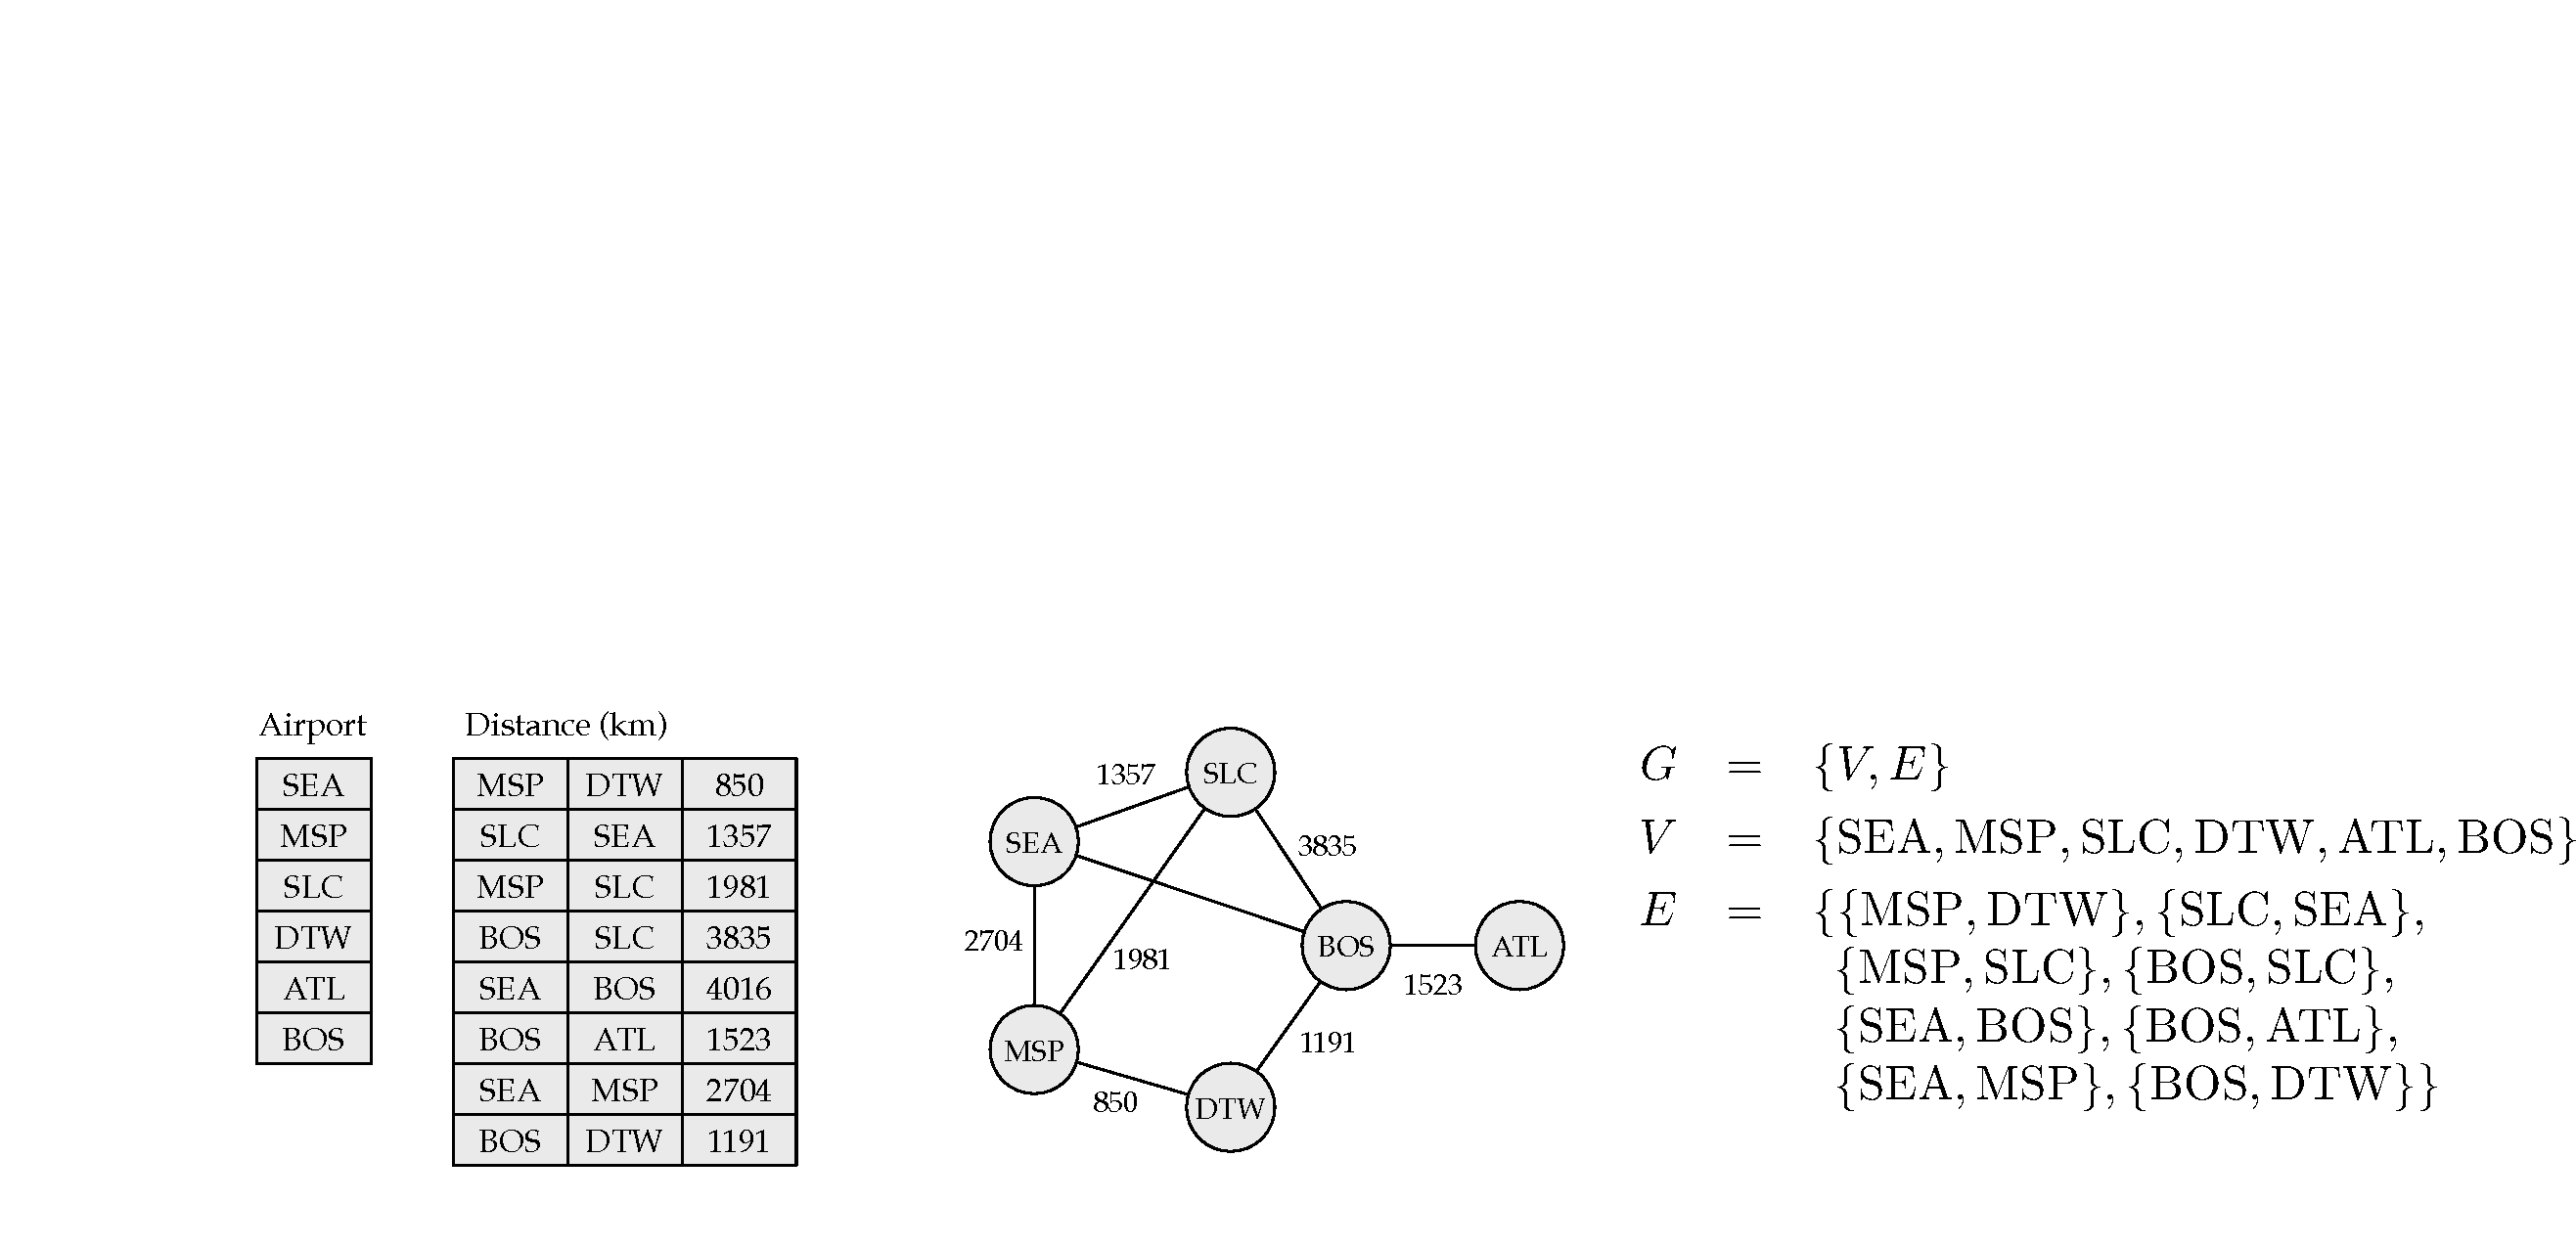
\includegraphics[width=0.75\textwidth]{figs/airport-summary.pdf}}
    \\
    \subcaptionbox{A directed graph representing an electronic circuit.  Shown in the circuit diagram are the labeled circuit nodes (the vertices) and the circuit elements connecting the nodes (the edges). Since circuit elements are oriented, we use a directed graph to model the circuit.  Also shown are a node and link diagram and the set-based description.\label{subfig:circuit}}
    {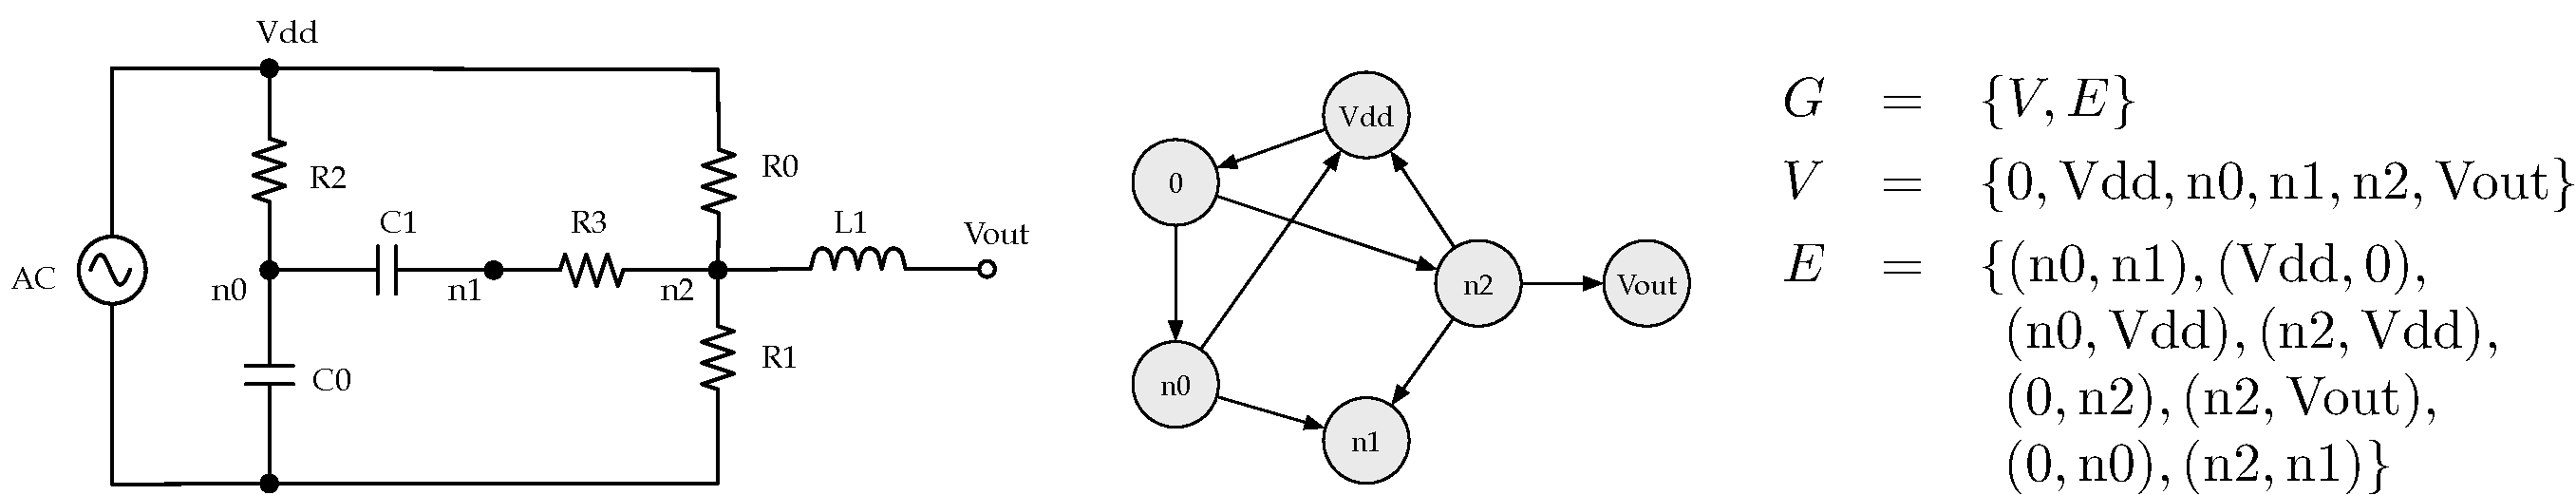
\includegraphics[width=0.825\textwidth]{figs/circuit-summary.pdf}}
    \caption{Graph models of an airline route system and of an electronic circuit.\label{fig:node_link_graphs}}
  \end{center}
\end{figure}


\subsection{Graph Representation: Enumerating the Vertices}

To reason about graphs, and to write algorithms for them, we require a \emph{representation} of the graph.
We note that \emph{a graph and its representation are not the same thing}.  It is therefore essential
that we be precise about this distinction as we develop a software library of graph
algorithms and data structures\footnote{In fact, if we are to be completely precise, the library we are
proposing is one of algorithms and data structures for graph representations.  We will make concessions
to commonly accepted terminology, while precisely defining that terminology.}.

The representations that we will be using are familiar ones: adjacency matrix, edge list, and adjacency list.
We begin with a process that is so standard that we typically don't even notice it, but it forms
the foundation of graph representations: we \emph{enumerate the vertices.}  That is, we assign an
index to each element of $V$ and write $V = \{v_0, v_1, \ldots v_{n-1}\}$.  Based on that enumeration,
elements of $E$ are expressed in the form $\{v_i, v_j\}$.  Similarly, we can enumerate the edges, and write  
$E = \{ e_0, e_1, \ldots e_{m-1}\}$, though the enumeration of $E$ does not play a role in standard
representations of graphs.
%
The number of elements in $V$ is denoted by $|V|$ and the number of elements in $E$ is denoted by $|E|$.

We summarize some remaining terminology about vertices and edges.
\begin{itemize}
\item 
An edge $e_k$ may  be \emph{directed}, denoted as the ordered pair $e_k=(v_i, v_j)$, or it may be
  \emph{undirected}, denoted as the (unordered) set $e_k=\{v_i, v_j\}$.  The edges 
in $E$ are either all directed or all undirected,
  corresponding respectively to a \emph{directed graph} or to an \emph{undirected} graph.
\item 
If the edge set $E$ of a directed graph contains an edge $e_k = (v_i,v_j)$, then
  vertex $v_j$ is said to be \emph{adjacent} to vertex $v_i$.  The edge $e_k$ is an
  \emph{out-edge} of vertex $v_i$ and an in-edge of vertex $v_j$.  Vertex $v_i$ is the \emph{source} of
  edge $e_k$, while $v_j$ is the \emph{target} of edge $e_k$.
\item If the edge set $E$ of an undirected graph contains an edge $e_k = \{v_i,v_j\}$, then
  $e_k$ is said to be \emph{incident} on the vertices $v_i$ and $v_j$.
  Moreover, vertex $v_j$ is adjacent to vertex $v_i$
  \emph{and} vertex $v_i$ is adjacent to vertex $v_j$.
  The edge $e_k$ is an out-edge of both $v_i$ and $v_j$ and it is an in-edge of both $v_i$ and $v_j$.
\item The \emph{neighbors} of a vertex $v_i$ are all the vertices $v_j$ that are adjacent to $v_i$.  The set of all of the neighbors is the \emph{neighborhood} of $v_i$.
\item A \emph{path} as a sequence of vertices $v_0, v_1, \ldots, v_{k-1}$ such that
there is an edge from $v_0$ to $v_1$, an edge from $v_1$ to $v_2$, and so on.
That is, a path is a set of edges $(v_i, v_{i+1}) \in E$ for  $i = 0, 1, \ldots, k-2$.
\end{itemize}


\subsection{Adjacency-Based Representations}

We begin our development of graph representations
with the almost universally-accepted definition of the
adjacency matrix representation of a graph.
%
The \emph{adjacency matrix representation} of a graph $G$ is a $|V|\times |V|$ matrix $A = (a_{ij})$ such that,
respectively for a directed or undirected graph
\[
 a_{i j} = 
 \left\{
 \begin{array}{rl}
  1 & \textrm{if } (v_i, v_j) \in E \\
  0 & \textrm { otherwise }
 \end{array}
 \right.
 \qquad\qquad
 a_{i j} = a_{ji} =
 \left\{
 \begin{array}{rl}
  1 & \textrm{if } (v_i, v_j) \in E \\ 
  0 & \textrm { otherwise }
 \end{array}
 \right.
\]
That is, $a_{ij} = 1$ if and only if $v_j$ is adjacent to $v_i$ in the original graph $G$ (hence the name ``adjacency matrix``).
%
Here we can see why we said that the initial enumeration of $V$ is foundational to representations:  \emph{The adjacency matrix is based solely on the indices used in that enumeration}.  It does not contain the vertices or edges themselves.

As a data structure to use for algorithms, the adjacency matrix is not very efficient, neither in terms of storage (which, at $|V|\times |V|$ is prohibitive), nor for computation. Instead of storing the entire
adjacency matrix, we can simply store the index values of its non-zero elements.  A \emph{sparse coordinate adjacency
matrix} is a container $C$ of pairs $(i, j)$ for every $a_{ij}$ in $A$.
%
At first glance, it may seem that we have simply created a data structure $C$ that has a pair $(i,j)$ if $E$ in the
original graph has an edge from $v_i$ to $v_j$.  This is true in the directed case.  However, in the undirected case, if there is an edge between $v_i$ and $v_j$, then $v_i$ is adjacent to $v_j$ and $v_j$ is adjacent to $v_i$.  In other words, if there is an edge between $v_i$ and  $v_j$ in an undirected graph, then both the entries $a_{ij}$ and $a_{ji}$ are equal to $1$\footnote{That is, the adjacency matrix is symmetric.} --- and therefore for a single edge between $v_i$ and $v_j$,  $C$ contains two index pairs: $(i, j)$  and $(j, i)$.   The sparse coordinate representation is commonly known as \emph{edge list}.  However, we caution the reader that $C$ does not store edges, but rather indices and that, in the case that it represents an undirected graph, there is not a 1-1 correspondence between the edges in $E$ and the contents of $C$.

Although the sparse coordinate adjacency matrix is much more efficient in terms of storage than the original adjacency matrix, it isn't as efficient as it could be.  
Much more importantly, it is not useful for the types of operations used by most graph algorithms, which need to be able to get the set of neighbors of a given vertex in constant time.  
To support this type of operation, we use a \emph{compressed sparse adjacency matrix}, which is an array $J$ with $|V|$ entries, where each $J[i]$ is a linear container of indices $\{ j \}$ such that $v_j$ is a neighbor of $v_i$ in $G$.  
That is $j$ is contained in $J[i]$ if and only if there is an edge $(v_i, v_j)$ in $E$ (or, equivalently, if there is a pair $(i, j)$ in $C$ or, equivalently, if $a_{ij} = 1$)\footnote{The compressed sparse adjacency matrix is identical to the compressed sparse row format from linear algebra}.  
We note that if $(v_i, v_j)$ is an edge in an undirected graph, $J[i]$ will contain $j$ and $J[j]$ will contain $i$. 
The common name for this data structure is \emph{adjacency list}.  
Although this name is problematic (for instance, it is not actually a list),  it is so widely used that we also use it here---but \emph{we mean specifically that an  ``adjacency list'' is the compressed sparse adjacency matrix representation of a graph}\footnote{We concede that ``adjacency list'' rolls off the tongue much more easily than ``compressed sparse adjacency matrix representation of a graph.''}.  
Again we emphasize the distinction between a graph and its representation:  An adjacency list $J$ is not the same as the graph $G$---it is a representation of $G$.


Illustrations of the adjacency-matrix representations of the airline route graph and the electronic circuit graph are shown in Figures~\ref{fig:airport} and~\ref{fig:circuit}, respectively.

\begin{figure}[tbh]
  \begin{subfigure}[t]{0.175\textwidth}
    \centering
    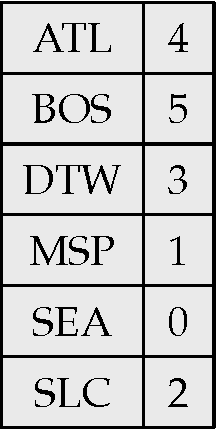
\includegraphics[width=0.4\linewidth]{airport-vertex-enumeration}
    \caption{\label{fig:airport-vertex-enumeration}
    An enumeration of the airport graph given in \protect\ref{subfig:airport}.}
  \end{subfigure}
  \hspace{1em}
  \begin{subfigure}[t]{0.25\textwidth}
    \centering
    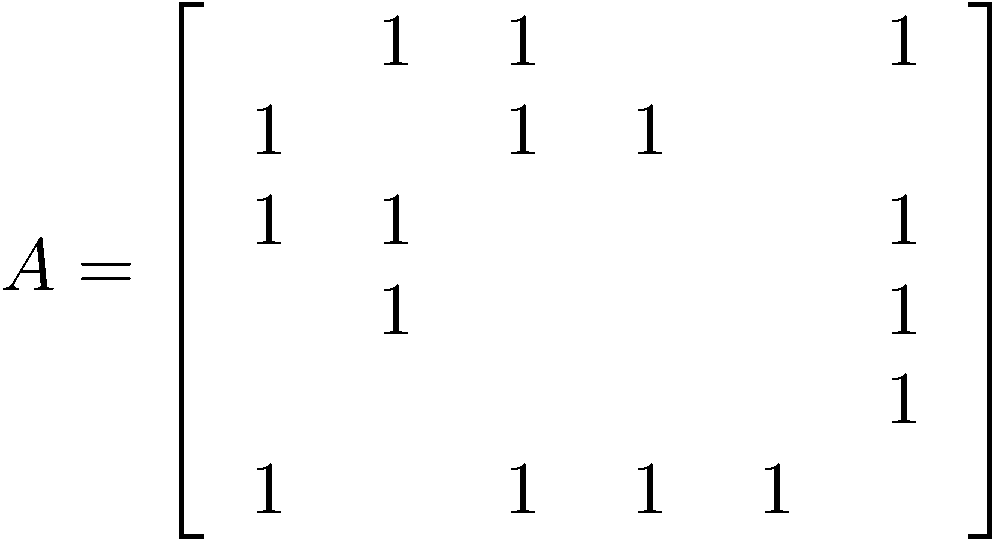
\includegraphics[width=\linewidth]{airport-graph-adjacency-matrix}
    \caption{\label{fig:airport-graph-adjacency-matrix}
    The adjacency matrix representation of the graph given in Figure~\protect\ref{subfig:airport},
    using the enumeration given in Figure~\protect\ref{fig:airport-vertex-enumeration}.}
  \end{subfigure}
  \hspace{1em}
  \begin{subfigure}[t]{0.175\textwidth}
    \small
    \centering
    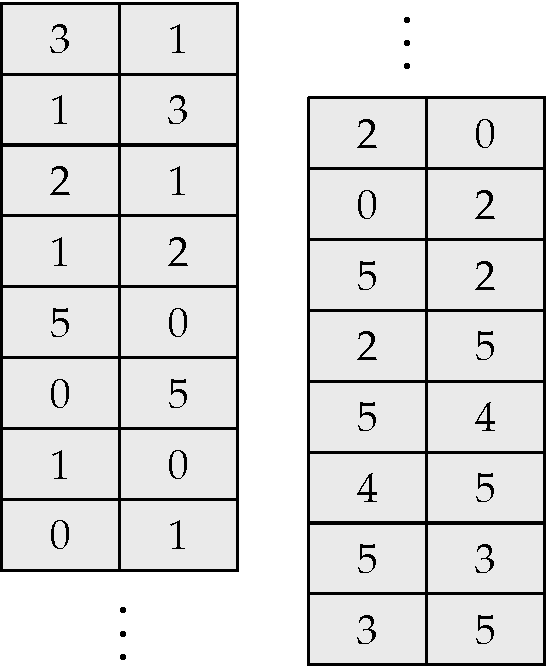
\includegraphics[width=0.7\linewidth]{split-airport-coordinate-sparse-adjacency}
    \caption{\label{fig:airport-coordinate-sparse-adjacency}
    The coordinate sparse adjacency matrix representation (shown split into two columns).}
  \end{subfigure}
  \hspace{1em}
  \begin{subfigure}[t]{0.3\textwidth}
    \small
    \centering
    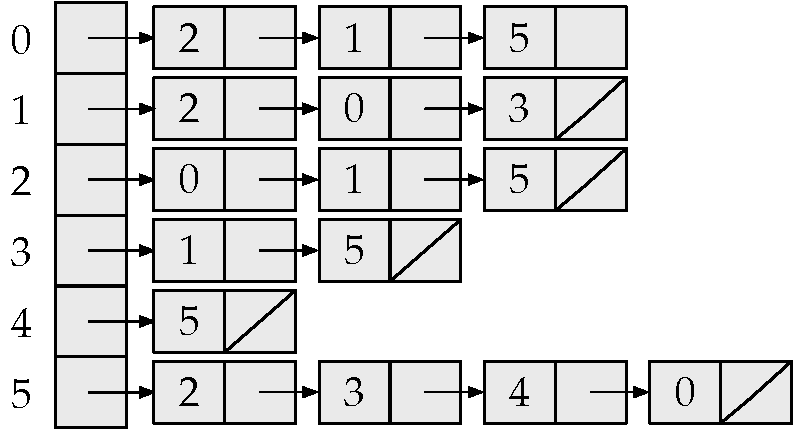
\includegraphics[width=0.75\linewidth]{airport-compressed-sparse-adjacency}
    \caption{\label{fig:airport-compressed-sparse-adjacency}
    The compressed sparse adjacency matrix representation.}
  \end{subfigure}
  \caption{Adjacency matrix representations of the airport graph model.\label{fig:airport-representation}}
\end{figure}



\begin{figure}[tbh]
  \begin{subfigure}[t]{0.175\textwidth}
    \centering
    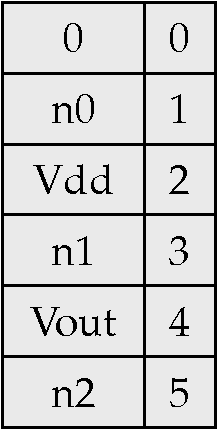
\includegraphics[width=0.4\linewidth]{circuit-vertex-enumeration}
    \caption{\label{fig:circuit-vertex-enumeration}
    An enumeration of the circuit graph given in \protect\ref{subfig:circuit}.}
  \end{subfigure}
  \hspace{1em}
  \begin{subfigure}[t]{0.25\textwidth}
    \centering
    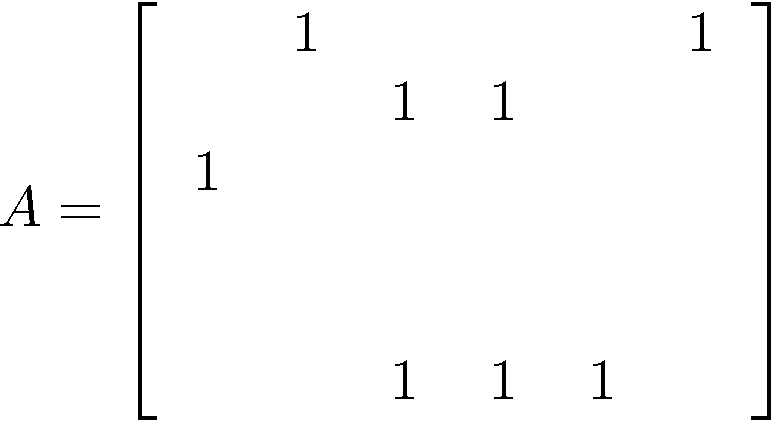
\includegraphics[width=\linewidth]{circuit-graph-adjacency-matrix}
    \caption{\label{fig:circuit-graph-adjacency-matrix}
    The adjacency matrix representation of the graph given in Figure~\protect\ref{subfig:circuit},
    using the enumeration given in Figure~\protect\ref{fig:circuit-vertex-enumeration}.}
  \end{subfigure}
  \hspace{1em}
  \begin{subfigure}[t]{0.175\textwidth}
    \small
    \centering
    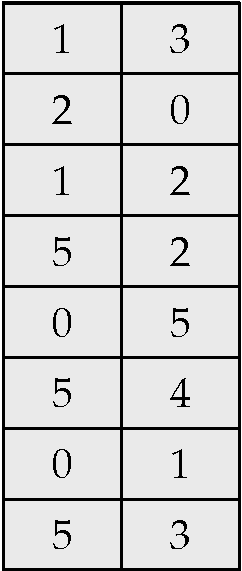
\includegraphics[width=0.4\linewidth]{circuit-coordinate-sparse-adjacency}
    \caption{\label{fig:circuit-coordinate-sparse-adjacency}
    The coordinate sparse adjacency matrix representation.}
  \end{subfigure}
  \hspace{1em}
  \begin{subfigure}[t]{0.3\textwidth}
    \small
    \centering
    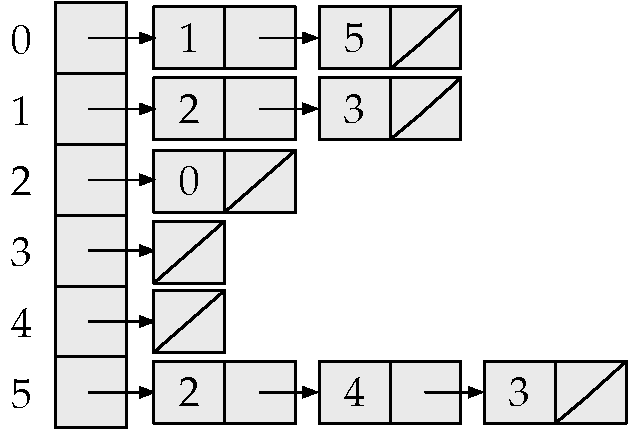
\includegraphics[width=0.75\linewidth]{circuit-compressed-sparse-adjacency}
    \caption{\label{fig:circuit-compressed-sparse-adjacency}
    The compressed sparse adjacency matrix representation.}
  \end{subfigure}
  \caption{Adjacency matrix representations of the circuit graph model.\label{fig:circuit-model}}
\end{figure}


\section{Bipartite Graphs}
\label{sec:bipartite}

\begin{figure}[ht]
 \begin{subfigure}[t]{0.15\textwidth}
    \small
    \centering
    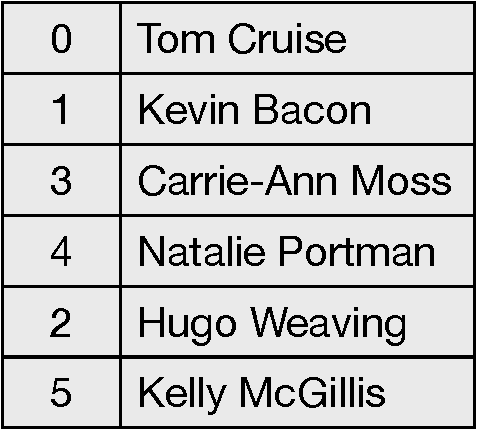
\includegraphics[width=0.825\linewidth]{figs/actor-table.pdf}
    \caption{\label{fig:actor-table}
    Table of actors.}
  \end{subfigure}
\hspace{1em}
   \begin{subfigure}[t]{0.167\textwidth}
    \small
    \centering
    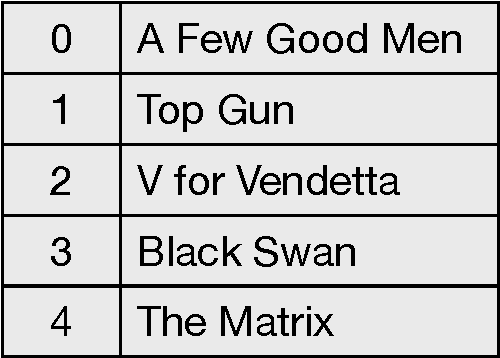
\includegraphics[width=0.825\linewidth]{figs/movie-table.pdf}
    \caption{\label{fig:movie-table}
    Table of movies.}
  \end{subfigure}
\hspace{1em}
     \begin{subfigure}[t]{0.3\textwidth}
    \small
    \centering
    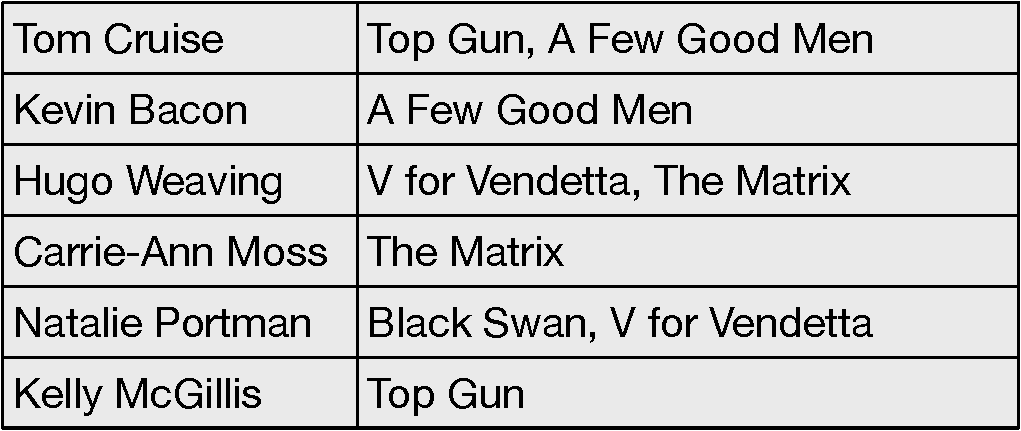
\includegraphics[width=0.825\linewidth]{figs/actor-movie-table.pdf}
    \caption{\label{fig:actor-movie-table}
    A table of actors and movies they have appeared in.}
  \end{subfigure}
\hspace{1em}
       \begin{subfigure}[t]{0.3\textwidth}
    \small
    \centering
    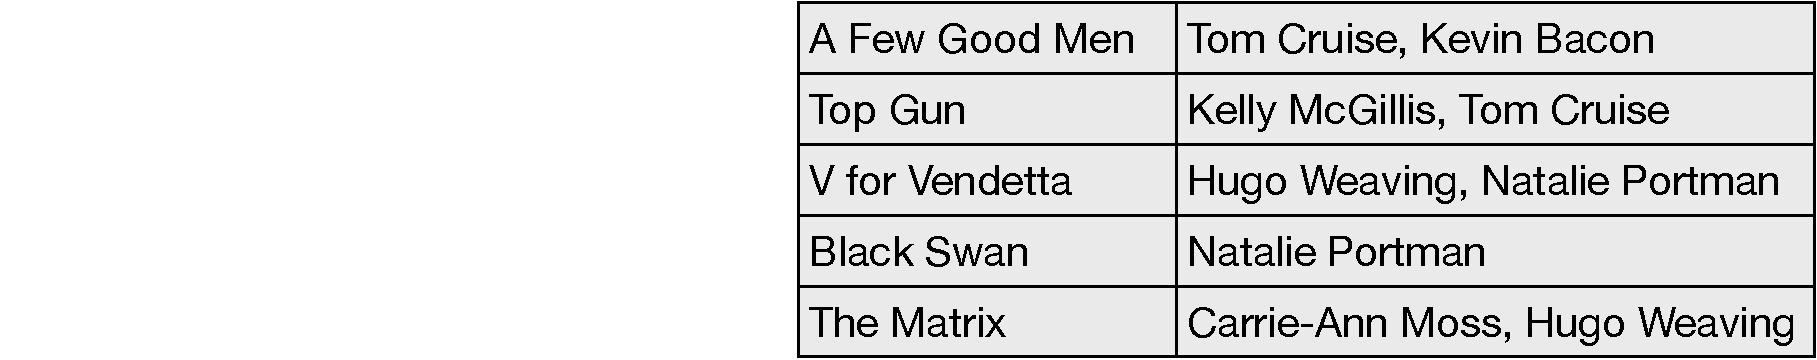
\includegraphics[width=0.9\linewidth]{figs/movie-actor-table.pdf}
    \caption{\label{fig:movie-actor-table}
    A table of movies with starring actors.}
  \end{subfigure}
  \caption{Illustrative simplification of IMDB actor and movie data.\label{fig:imdb}}

\end{figure}

So far, we have been considering graphs where 
edges in $E$ are pairs of vertices, which are taken from a single set $V$.
%
We refer to such a graph as a \emph{unipartite} graph.
%
But consider again the Kevin Bacon example.  The source for the information comprising the Kevin Bacon data is the Internet Movie Database (IMDB).  
However, the IMDB does not contain any explicit information about the relationships between actors.  
%
Rather it contains files of tabular data, one of which contains an entry for each movie with the list of actors that have appeared in that movie,
and another of which contains an entry for each actor with the list of movies that actor has
appeared in (``movie-actor'' and ``actor-movie'' tables, respectively).  Such tables are shown in Figure~\ref{fig:imdb}.\footnote{This is a greatly simplified version of the CSV files that actually comprise the IMDB.  The full set of files is available for non-commercial use at~\url{https://datasets.imdbws.com}.}
%
Thus, a graph, as we have defined it, cannot model the IMDB.  

There is a small generalization we can make to the definition of graph that will result in a suitable abstraction for modeling the IMDB.  In particular, we need one set of vertices corresponding to actors, another set of vertices corresponding to movies, and then a set of edges corresponding to the relationships between actors and movies.  There are two kinds of relationships to consider actors in movies or movies starring actors.  To be well-defined, the edge set may only contain one kind of relationship.  To capture this kind of model, we define a \emph{structurally bipartite graph} $H = \{ U, V, E \}$, where vertex sets $U$ and $V$ are enumerated $U = \{ u_0, u_1, \ldots , u_{n0} \}$ and $V  = \{ v_0, v_1, \ldots v_{n1}\}$, 
and the edge set $E$ consists of pairs $(u_i, v_j)$ where $u_i$ is in $U$ and $v_j$ is in $V$.

The \emph{adjacency matrix representation of a structurally bipartite graph} is
a $|U|\times |V|$ matrix $A = (a_{ij})$ such that,
\[
 a_{i j} = 
 \left\{
 \begin{array}{rl}
  1 & \textrm{if } (v_i, v_j) \in E \\
  0 & \textrm { otherwise }
 \end{array}
 \right.
 \]
From this adjacency matrix representation we can readily construct  coordinate and compressed sparse representations.  The only structural difference between the representations of a structurally bipartite graph and that of a unipartite graph is that of vertex cardinality.  That is, in a unipartite graph, edges map from $V$ to $V$, and hence the values in the left hand column and in the right hand column of a coordinate representation would be in the same range: $[0, |V|)$.  However, for a structurally bipartite graph, this is no longer the case.  Although the coordinate representation still consists of pairs of vertex indices, the range of values in the left hand column is $[0, |U|)$, while in the right hand column it is $[0, |V|)$.  Similarly, the compressed representation will have $|U|$ entries, but the values stored in each entry may range from $[0, |V|)$.  We note that these are constraints on values, not on structure.
 

\begin{figure}[ht]
 \begin{subfigure}[t]{0.4\textwidth}
    \small
    \centering
    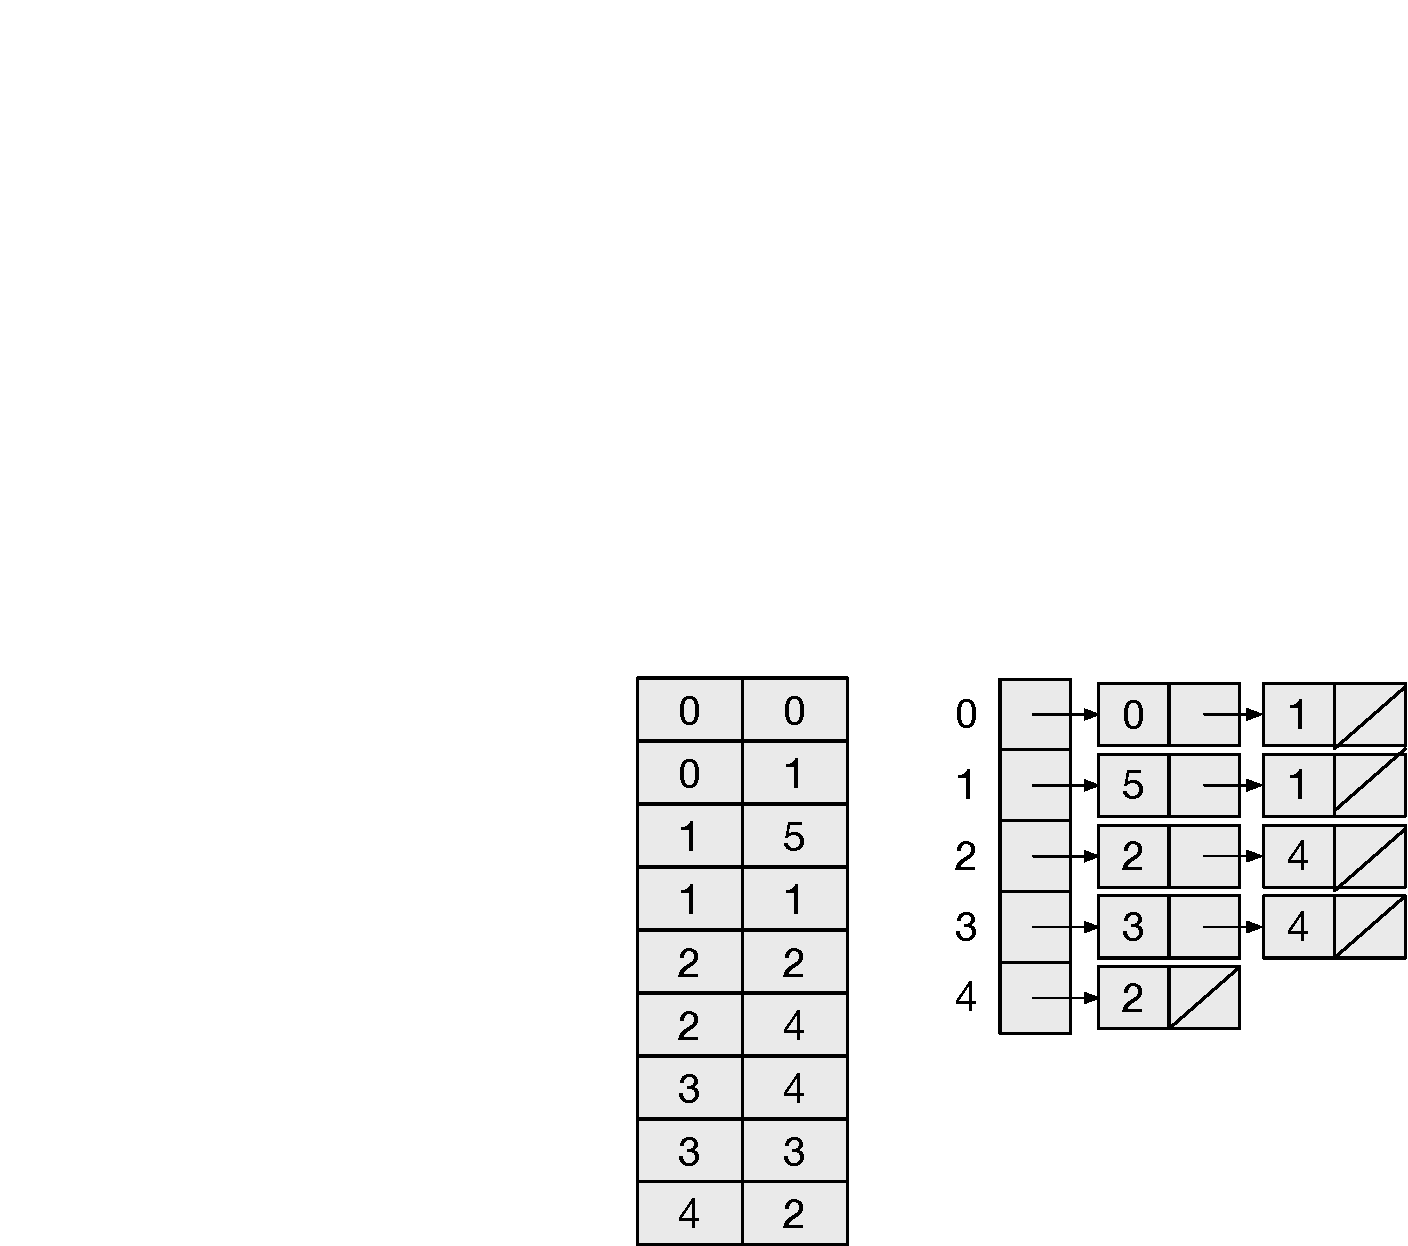
\includegraphics[width=0.825\linewidth]{figs/movie-actor-sparse-adjacency}
    \caption{\label{fig:actor-table}
    Coordinate and compressed sparse adjacency representations for movies with their starring actors.}
  \end{subfigure}
\hspace{1em}  
   \begin{subfigure}[t]{0.4\textwidth}
    \small
    \centering
    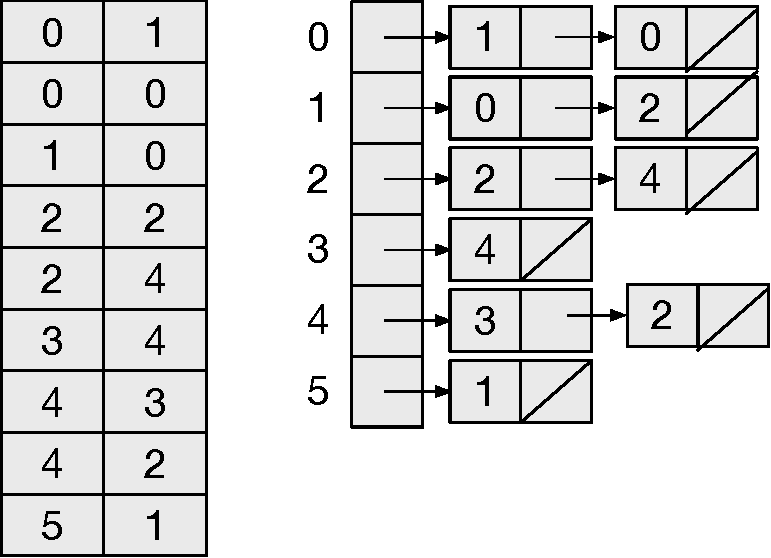
\includegraphics[width=0.825\linewidth]{figs/actor-movie-sparse-adjacency}
    \caption{\label{fig:movie-table}
    Coordinate and compressed sparse adjacency representations for actors and the movies they have appeared in.}
  \end{subfigure}
  \caption{Sparse adjacency representations (edge lists and adjacency lists) for IMDB actor and movie data.}
\end{figure}

We distinguish a structurally bipartite graph from simply a bipartite graph because the former applies separate enumerations to $U$ and $V$.  
In customary graph terminology, a \emph{bipartite} graph is one in which the vertices can be partitioned into two disjoint sets, such that all of the edges in the graph only connect vertices from one set to vertices of the other set.  However, although the vertices are partitioned, they are still taken from the same original vertex set $V$ and have a single enumeration.
Whether a graph can be partitioned in this way is a run-time property inherent to the graph itself (which can be discovered with an appropriate algorithm).  
This is not a natural way to model separate categories of entities, such as movies and actors, where entities are categorized completely independently of each other and it is therefore most appropriate to have independent enumerations for them.  
A structurally bipartite graph explicitly captures distinct vertex categories.
%

\section{Partitioned Graphs}

In contrast to structurally bipartite graphs, there are certainly cases
where one would want to maintain two categories of entities, or otherwise distinguish the vertices, from the same vertex set.  In that case, we would use a \emph{partitioned graph}, which we define as
$G = \{ V, E \}$, where the vertex set $V$ consists of non-overlapping subsets, i.e.,
$V = \{ V_0, V_1, \ldots \}$ which we enumerate as $V_0 = \{v_0, v_1, \ldots , v_{n0-1} \}$, 
$V_1 = \{ v_{n0}, \ldots , v_{n1-1} \}$ and so on.  Each $V_i$ is a \emph{partition} of $V$.
The total enumeration of $V$ is $V= \{ v_0, v_1, \ldots , v_{n-1} \}$.  Just as each $V_i$ is a partition of $V$, the enumeration of each $V_i$ is a partitioning of the enumeration of $V$.

The edge set $E$ still consists of edges $(v_i, v_j)$ (or $\{v_i, v_j\}$ where, in general, $v_i$ and $v_j$ may come from any partition.

We note that partitioned graphs are not restricted to two partitions---a partitioned graph can represent an arbitrary number of partitions, i.e., a \emph{multipartite} graph (a graph with multiple subsets of vertices such that edges only go between subsets).
While partitioned graphs can be used to model multipartite graphs, partitioned graphs are not necessarily multipartite; edges can comprise vertices within a partition as well as well as across partitions.


\section{From Data to Graph}

\subsection{Columnar Data}
Here we show how one might create an unlabeled edge list from a table of data stored in a CSV file.  The following loads a list of directed edges from a CSV file (the values in each row are assumed to be separated by whitespace)\footnote{We take a broad view of what a comma is.}.
The elements of the first column are considered to be the source vertices and the elements of
the second column are the destination vertices. If the edges also had properties, the third column
would contain the property values.  In this example, the edges are loaded into a vector of tuples, which meets the requirements of a (presumed) \lstinline{sparse_coordinate} concept.
\begin{lstlisting}[language=C++]
    auto sparse_coordinate edges = std::vector<std::tuple<vertex_id_t, vertex_id_t>;
    auto input = std::ifstream ("input.csv");
    vertex_id_t src, dst;
    while (input >> src >> dst) {
        edges.emplace_back (src, dst);
    }
\end{lstlisting}

Similarly, we could load a list of undirected edges from a CSV file into a 
\lstinline{sparse_coordinate} structure.  
Note that, as discussed above, the coordinate sparse adjacency matrix representation (aka an edge list), contains an entry $(i, j)$ as well as an entry $(j, i)$ for each undirected edge $\{ v_i, v_j \}$.  Hence, we add both \lstinline{(src, dst)} and  \lstinline{(dst, src)} to \lstinline{edges}.
\begin{lstlisting}[language=C++]
    auto sparse_coordinate edges = std::vector<std::tuple<vertex_id_t, vertex_id_t, double> edges;
    auto input = std::ifstream ("input.csv");
    vertex_id_t src, dst;
    double val;
    while (input >> src >> dst >> val) {
        edges.emplace_back (src, dst, val);
        edges.emplace_back (dst, src, val);
    }
\end{lstlisting}

These examples are meant to be illustrative and not necessarily
comprehensive (nor efficient).
There are, of course, many ways to define containers that meet the
requirements of the edge list concept and many ways to
create an edge list from columnar data.

\subsection{Converting an Edge List to an Adjacency List}

The following creates a compressed sparse representation (an adjacency list) from a coordinate sparse representation.  The adjacency list is represented as 
a \lstinline{std::vector<std::vector<vertex_id_t>>;}
\begin{lstlisting}[language=C++]
    auto sparse_coordinate edges = std::vector<std::tuple<vertex_id_t, vertex_id_t>;
    // Read the edges
    auto sparse_compressed adj_list = std::vector<std::vector<vertex_id_t>>;
    for (auto [src, dst] : edges) {
      if (src >= adj_list.size()) {
        adj_list.resize(src + 1);
      }
      adj_list[src].push_back (dst);
    }
\end{lstlisting}

We note that the \lstinline{sparse_coordinate} representation is agnostic as to whether it was originally created based on directed edges or undirected edges.  An optimization to the sparse coordinate representation would be to use a \emph{packed coordinate} representation, which would only maintain a single entry for each undirected edge.  In that case, we would need to have two complementary insertions into the adjacency list for each entry in the packed coordinate representation.

The following example illustrates the use of a packed coordinate format to construct an adjacency list with an edge property.
\begin{lstlisting}[language=C++]
    auto packed_sparse_coordinate edges = std::vector<std::tuple<vertex_id_t, vertex_id_t, double>>;
    // Read the edges
    auto compressed_sparse adj_list = std::vector<std::vector<std::tuple<vertex_id_t, double>>>(edges.num_vertices();
    for (auto [src, dst, val] : edges) {
      adj_list[src].push_back (dst, val);
      adj_list[dst].push_back (src, val);
    }
 \end{lstlisting}

% \andrew{We should have note that anything wrapped in a graph adapter has a `num\_vertices`
% method (and other members).
% We should also provide a constructor for the adapted adjacency list that takes and
% edge list as argument.}


% The examples above basically cover what I intened here.  Though perhaps we should
% explain in some more detail about what the concepts do, what kinds of things meet
% concept requirements, what the graph adapter does, etc.
% \section{Implementations}
% But maybe we can just cover those things further down and forward reference to
% them from here.

% \subsection{Edge List: Array of Structs / Struct of Arrays}
% \andrew{Edges can be stored as tuples (or tuple like) basically in parallel arrays (like a ranges::zip).}
% \subsection{Vertices and Edges: Node Objects and Link Objects}
% \andrew{ala Stanford Graph Base (et al).}
% \subsection{Adjacency List: Container of Containers}
% \andrew{An adjacency list can be represented as a container of containers (e.g., std::vector<std::list>).  Talk about range of ranges when we talk about library interfaces, requirements, concepts.  Note here that the structure of an adjacency list does not capture directedness -- directedness is a run-time property.}


% These are definitely already covered in the examples above.
% \subsection{From Edge List to Adjacency List}
% \andrew{Scan edge list and insert edgest into adjacency list.  Adjacency list must support insertion.}
% \subsection{Edge List and Adjacency List: Compressed Edge List}
% \andrew{Using a sort and group-by (or a sort, a run-length encoding, and a scan), we can compactify the edge-list reprentation and at the same time obtain an adjacency-list representation -- one that is memory and compute efficient.  Best of both worlds.  Has same basic structural principles as CSR / CSC matrices in linear algebra -- but much more general.}



%% \chapter{Algorithms}

\section{Algorithm Selection} \label{other_algo}

When determining the algorithms to propose we split them into different tiers. Tier 1 algorithms are included
in this proposal. The algorithms selected are a result of balancing a few things:
\begin{itemdescr}
\begin{itemize}
      \item Include a rich enough set of algorithms for the library to be useful.
      \item Include algorithms with well-defined functionality and agreed-upon algorithmic description.
      \item Don't include so many that the proposal will get bogged down for years and years.
\end{itemize}
\end{itemdescr}

\subsection{Tier 1 Algorithms}
\begin{multicols}{3}
      \emph{Shortest Paths}
      \begin{itemize}
            %\item Shortest paths (driver interface)
            \item Breadth-First search
            \item Dijkstra's algorithm
            \item Bellman-Ford
      \end{itemize}
      \emph{Clustering}
      \begin{itemize}
            \item Triangle counting
      \end{itemize}
      \emph{Communities}
      \begin{itemize}
            \item Label propagation
      \end{itemize}
\columnbreak
      \emph{Components}
      \begin{itemize}
            \item Articulation points
            \item Connected components
            \item Biconnected components
            \item Kosaraju's Strongly CC
            \item Tarjan's Strongly CC
      \end{itemize}
      \emph{Directed Acyclic Graphs}
      \begin{itemize}
            \item Topological sort
      \end{itemize}
\columnbreak
      \emph{Maximal Independent Set}
      \begin{itemize}
            \item Maximal independent set
      \end{itemize}
      \emph{Link Analysis}
      \begin{itemize}
            \item Jaccard coefficient
      \end{itemize}
      \emph{Minimal Spanning Tree}
      \begin{itemize}
            \item Kruskal's MST
            \item Prim's MST
      \end{itemize}

\vfill\null
\end{multicols}

Shortest Paths and Topological Sort are all single source with multiple targets.

\subsection{Other Algorithms}
Additional algorithms that were considered but not included in this proposal are shown in Table \ref{tab:other_algorithms}. 
Tier X algorithms are variations of shortest paths algorithms that complement the Single Source, Multiple Target algorithms 
in this proposal.
It is assumed that future proposals will include them, thought the exact mix for each proposal will depend on feedback received
and our experience with the current proposal.

\phil{We may want to revisit the Driver idea in the future after we have more algorithms.}
%The Shortest Paths Driver is an idea of having a unified interface that chooses the best Shortest Path algorithm
%based on characteristics like non-negative edge weight, multi-threading, etc.

\begin{table}[h!]
\begin{center}
%\resizebox{\textwidth}{!}
{\begin{tabular}{l|l|l}
\hline
    \textbf{Tier 2} & \textbf{Tier 3} & \textbf{Tier X} \\
\hline
    All Pairs Shortest Paths & Jones Plassman & Single Source, Single Target: Shortest Paths Driver\\
    Floyd-Warshall & Cores: k-cores & Single Source, Single Target: BFS \\
    Johnson & Cores: k-truss & Single Source, Single Target: Dijkstra \\
    Centrality: Betweenness Centrality & Subgraph Isomorphism & Single Source, Single Target: Bellman-Ford \\
    Coloring: Greedy & & Single Source, Single Target: Delta Stepping \\
    Communities: Louvain & &  \\
    Connectivity: Minimum Cuts & & Multiple Source: Shortest Paths Driver \\
    Transitive Closure & & Multiple Source: BFS \\
    Flows: Edmunds Karp & & Multiple Source: Dijkstra \\
    Flows: Push Relabel & & Multiple Source: Bellman-Ford \\
    Flows: Boykov Kolmogorov & & Multiple Source: Delta Stepping \\
    Link Analysis: Adamic-Adar Index & &  \\
    Pathfinding: A* & & Multiple Source, Single Target: Shortest Paths Driver\\
    Best-first search & & Multiple Source, Single Target: BFS \\
    & & Multiple Source, Single Target: Dijkstra \\
    & & Multiple Source, Single Target: Bellman-Ford \\
    & & Multiple Source, Single Target: Delta Stepping \\
\hline
\end{tabular}}
\caption{Other Algorithms}
\label{tab:other_algorithms}
\end{center}
\end{table}

\andrew{All Pairs: Tier 2?  People bring this up alot -- but it is very expensive in terms of computation and memory.}
\phil{If it's useful to enough people it should be included. Users can make their own determination of whether they want to use it, based on the cost.}

\andrew{Note that NetworkX also specifies single source single target and multiple source versions of the shortest paths algorithms.  
BGL does not have these (nor NWGraph).  We should discuss whether or not to consider those and whether or not to make them Tier 1, 2, 3, or infinity.}
\phil{I think we're beyond considering these for the initial proposal. They can be added in the future, unless we're told otherwise.}

\phil{The same variations for Shortest Paths algorithms can also be useful for topological sort.}

\phil{Many algorithms allocate memory. Should we include a [PMR] allocator argument?}

% Floyd-Warshall $\mathcal{O}(N^2)$}
% Johnson $\mathcal{O}(N^2)$}

\section{Algorithm Concepts}

%\andrew{Need to develop this ala CppCon 2021 talk.}

The abstraction that is used for describing and analyzing almost all graph algorithms is the adjacency list.  Naturally then implementations of graph algorithms in C++ will operate on a data structure representing an adjacency list.  And generic algorithms will be written in terms of concepts that capture the essential operations that a concrete data structure must provide in order to be used as an abstraction of an adjacency list.

Most fundamentally (as illustrated above), an adjacency list is a collection of vertices, each of which has a collection of outgoing edges.  In terms of existing C++ concepts, we can consider an adjacency list to be a range of ranges (or, more specifically, a random access range of forward ranges).  The outer range is the collection of vertices, and the inner ranges are the collections of outgoing edges.

%\andrew{Is it better to list the concepts here or forward reference them?  Kind of a circularity.  But maybe the sequence of concepts - algorithms - concrete data types is the right one.  OTOH, std::ranges use ordering overview library-concepts-containers-algorithms.  Since a graph is a range of ranges, maybe we should follow that.}

%\phil{I think this is a good place, just before they're used in the text for this section.}
% Additional concepts used by algorithms.

\begin{lstlisting}
template <class G, class WF, class DistanceValue, class Compare, class Combine>
concept basic_edge_weight_function = // e.g. weight(uv)
      is_arithmetic_v<DistanceValue> && 
      strict_weak_order<Compare, DistanceValue, DistanceValue> &&
      assignable_from<add_lvalue_reference_t<DistanceValue>,
            invoke_result_t<Combine, DistanceValue, invoke_result_t<WF, edge_reference_t<G>>>>;

template <class G, class WF, class DistanceValue>
concept edge_weight_function = // e.g. weight(uv)
      is_arithmetic_v<invoke_result_t<WF, edge_reference_t<G>>> &&
      basic_edge_weight_function<G,
                                  WF,
                                  DistanceValue,
                                  less<DistanceValue>,
                                  plus<DistanceValue>>;
\end{lstlisting}

\begin{comment}
      \phil{Queueable isn't being used.}
      \begin{lstlisting}
      // queueableQ can represent std::queue and std::priority\_queue
      template <class Q>
      concept queueable = requires(Q&& q, Q::value_type value) {
      Q::value_type;
      Q::size_type;
      Q::reference;

      {q.top()};
      {q.push(value)};
      {q.pop()};
      {q.empty()};
      {q.size()};
      };
      \end{lstlisting}
\end{comment}



\section{Shortest Paths}


\begin{comment}
      \subsection{Driver Interface}

      \andrew{I am not sure we should have the unified interface.  We need to be more parsimonious in our interfaces.  Users can read the documentation for which algorithms to use.  And, if they are using graph algorithms, we should assume a certain level of knowledge about graph algorithms.  OTOH, it is only a handful of algorithms.}

      \andrew{I am also not sure we should have ``shortest distance'' variants.  That doubles the number of functions in the interface.
            For each function we have shortest paths, s-t paths, multi-source paths, parallel = 6X variants for each base function.  If we add shortest distances, that will make 12X.  OTOH, we could consider not having s-t paths or not having multi-source paths -- which would leave 4X for each base function.  However, I think people will want s-t and multi-source.
      }
      \phil{\tcode{dijkstra_shortest_distances} includes predecessor and distances, so excluding \tcode{dijkstra_shortest_distances} won't impact 
      the user much.}


      {\small
            \lstinputlisting{D9902/src/shortest_paths.hpp}
      }

      \andrew{The variety of algorithms was inspired by networkx....  Which also had ``distance'' variants.}

      \phil{I assume \tcode{adjacency_list_graph} is the same as our \tcode{adjacency_list}. \tcode{bidirectional_adjacency_list_graph} is new; what to do with it?}
\end{comment}


\subsection{Unweighted Shortest Paths}

\subsubsection{Breadth-First Search, Single Source, Initialization}

{\small
      \lstinputlisting{D9902/src/breadth_first_search_helpers.hpp}
}

\begin{itemdescr}
      \effects
      \begin{itemize}
            \item
                  Each \lstinline{predecessors[i]} is initialized to \lstinline{i}.
      \end{itemize}
\end{itemdescr}


\subsubsection{Breadth-First Search, Single Source}
Compute the breadth-first path and associated distance from vertex \tcode{source} to all reachable vertices in \tcode{graph}.

\begin{table}[h]
\setcellgapes{3pt}
\makegapedcells
\centering
\begin{tabular}{|P{0.30\textwidth}|P{0.25\textwidth}|P{0.25\textwidth}|}
\hline
      \multirowcell{2}{
            \textbf{Complexity} \\
                  $\mathcal{O}((|E| + |V|)\log{|V|})$
            }
      & \textbf{Throws?} No & \textbf{Cycles?} No \\
      & \textbf{Multi-edge?} No & \textbf{Directed?} Yes \\
\hline
\end{tabular}
%\caption{Dijkstra Single Source Summary}
\label{tab:dijkstra_ss_summary}
\end{table}
Note that complexity may be $\mathcal{O}(|E| + |V|\log{|V|)}$ for certain implementations.

{\small
      \lstinputlisting{D9902/src/breadth_first_search.hpp}
}

\begin{itemdescr}
      %\pnum\mandates
      % \pnum
\preconditions
            \begin{itemize}
                  \item
                        \lstinline{0 <= source < num_vertices(graph)}. 
                  \item
                        \lstinline{distances} will be initialized with \lstinline{init_breadth_first_search}.
                  \item
                        \lstinline{predecessors} will be initialized with \lstinline{init_breadth_first_search}.
            \end{itemize}
      \pnum\effects
            \begin{itemize}
                  \item
                        If vertex with index \lstinline{i} is reachable from vertex \lstinline{source}, then
                        \lstinline{distances[i]} will contain the lowest number of edges from \lstinline{source} to vertex
                        \lstinline{i}.  Otherwise \lstinline{distances[i]} will contain
                        \lstinline{breadth_first_search_invalid_distance()}.
                  \item
                        If vertex with index \lstinline{i} is reachable
                        from vertex \lstinline{source}, then \lstinline{predecessors[i]} will contain the
                        predecessor vertex of vertex \lstinline{i}. Otherwise \lstinline{predecessors[i]} will contain
                        \lstinline{i}.
            \end{itemize}
      %\pnum\result
      %\pnum\returns \lstinline{void} \\
      %\pnum\throws \tcode{out_of_range} is thrown when \tcode{source} is not in the range \tcode{0 <= source < num_vertices(graph)}.  \\
      %\pnum\complexity \\
      %\pnum\remarks 
      %\pnum\errors
\end{itemdescr}


\subsection{Weighted Shortest Paths}

\subsubsection{Shortest Paths Initialization}

{\small
      \lstinputlisting{D9902/src/shortest_paths_helpers.hpp}
}

\begin{itemdescr}
      \pnum
      \effects:
            \begin{itemize}
                  \item
                        \lstinline{init_shortest_paths(distances)} sets all elements in \lstinline{distance} to \lstinline{shortest_path_invalid_distance()}
                  \item
                        \lstinline{init_shortest_paths(distances,predecessors)} does the same as \lstinline{shortest_path_invalid_distance(distances)}
                        and sets \lstinline{predecessors[i] = i} for \lstinline{i < size(predecessors)}.
            \end{itemize}
      \pnum\returns 
            \begin{itemize}
                  \item \lstinline{shortest_path_invalid_distance()} returns a sentinel value for an invalid distance,
                        typically \lstinline{numeric_limits<DistanceValue>::max()} for numeric types.
                  \item \lstinline{shortest_path_zero()} returns a value for for a zero-length path,
                        typically \lstinline{0} for numeric types.
            \end{itemize}
\end{itemdescr}


\subsubsection{Dijkstra Single Source Shortest Paths and Shortest Distances}

Compute the shortest path and associated distance from vertex \tcode{source} to all reachable vertices in \tcode{graph}
using non-negative weights.

\begin{table}[h]
\setcellgapes{3pt}
\makegapedcells
\centering
\begin{tabular}{|P{0.30\textwidth}|P{0.25\textwidth}|P{0.25\textwidth}|}
\hline
      \multirowcell{2}{
            \textbf{Complexity} \\
                  $\mathcal{O}((|E| + |V|)\log{|V|})$
            }
      & \textbf{Throws?} No & \textbf{Cycles?} No \\
      & \textbf{Multi-edge?} No & \textbf{Directed?} Yes \\
\hline
\end{tabular}
%\caption{Dijkstra Single Source Summary}
\label{tab:dijkstra_ss_summary}
\end{table}
Note that complexity may be $\mathcal{O}(|E| + |V|\log{|V|)}$ for certain implementations.

The following functions are split into the common and general cases, where the general cases allow the caller
to specify \tcode{Compare} and \tcode{Combine} functions (e.g. less and add). Concepts and types from 
\tcode{std::ranges} don't include the namespace prefix for brevity and clarity of purpose.

{\small
      \lstinputlisting{D9902/src/dijkstra_common.hpp}
      \lstinputlisting{D9902/src/dijkstra_general.hpp}
}

\begin{itemdescr}
      \pnum\mandates
            \begin{itemize}
                  \item
                        The weight function \lstinline{w} must return a non-negative value.
            \end{itemize}
      \pnum\preconditions
            \begin{itemize}
                  \item
                        \lstinline{0 <= source < num_vertices(graph)}. 
                  \item
                        \lstinline{distances} will be initialized with \lstinline{init_shortest_paths}.
                  \item
                        \lstinline{predecessors} will be initialized with \lstinline{init_shortest_paths}.
            \end{itemize}
      \pnum\effects
            \begin{itemize}
                  \item
                        If vertex with index \lstinline{i} is reachable from vertex \lstinline{source}, then
                        \lstinline{distances[i]} will contain the distance from \lstinline{source} to vertex
                        \lstinline{i}.  Otherwise \lstinline{distances[i]} will contain
                        \lstinline{shortest_path_invalid_distance()}.
                  \item
                        If vertex with index \lstinline{i} is reachable
                        from vertex \lstinline{source}, then \lstinline{predecessors[i]} will contain the
                        predecessor vertex of vertex \lstinline{i}. Otherwise \lstinline{predecessors[i]} will contain
                        \lstinline{i}.
            \end{itemize}
      %\pnum\result
      %\pnum\returns \lstinline{void} \\
      %\pnum\throws \tcode{out_of_range} is thrown when \tcode{source} is not in the range \tcode{0 <= source < num_vertices(graph)}.  \\
      %\pnum\complexity \\
      \pnum\remarks 
                        Bellman-Ford Shortest Paths allows negative weights with the consequence of greater complexity. \\
      %\pnum\errors
\end{itemdescr}


\subsubsection{Bellman-Ford Single Source Shortest Paths and Shortest Distances}
Compute the shortest path and associated distance from vertex \tcode{source} to all reachable vertices in \tcode{graph}.


\begin{table}[h]
      \setcellgapes{3pt}
      \makegapedcells
      \centering
      \begin{tabular}{|P{0.30\textwidth}|P{0.25\textwidth}|P{0.25\textwidth}|}
      \hline
            \multirowcell{2}{
                  \textbf{Complexity} \\
                        $\mathcal{O}(|E| \cdot |V|)$ \\
                  }
            & \textbf{Throws?} No & \textbf{Cycles?} No \\
            & \textbf{Multi-edge?} No & \textbf{Directed?} Yes\\
      \hline
      \end{tabular}
      %\caption{Bellman-Ford Single Source Summary}
      \label{tab:bellford_ss_summary}
\end{table}
%\andrew{Complexity is really is atrocious.  Suitable only for really small graphs.}


The following functions are split into the common and general cases, where the general cases allow the caller
to specify \tcode{Compare} and \tcode{Combine} functions (e.g. less and add). Concepts and types from 
\tcode{std::ranges} don't include the namespace prefix for brevity and clarity of purpose.

{\small
      \lstinputlisting{D9902/src/bellman_ford_common.hpp}
      \lstinputlisting{D9902/src/bellman_ford_general.hpp}
}

\phil{Should negative weight cycles be a pre-condition, or should it be detected with an exception thrown when it exists?}

\phil{NetworkX has \tcode{negative_edge_cycle} and \tcode{find_negative_cycle}. These are needed if negative weight cycles are a pre-condition?}

\begin{itemdescr}
      %\pnum\mandates
      \pnum\preconditions
            \begin{itemize}
                  \item
                        \lstinline{0 <= source < num_vertices(graph)}. 
                  \item
                        \lstinline{distance} will be initialized with \lstinline{init_shortest_paths}.
                  \item
                        \lstinline{predecessors} will be initialized with \lstinline{init_shortest_paths}.
            \end{itemize}
      \pnum\effects
            \begin{itemize}
                  \item
                        If vertex with index \lstinline{i} is reachable from vertex \lstinline{source}, then
                        \lstinline{distances[i]} will contain the distance from \lstinline{source} to vertex
                        \lstinline{i}.  Otherwise \lstinline{distances[i]} will contain
                        \lstinline{shortest_path_invalid_distance()}.
                  \item
                        If vertex with index \lstinline{i} is reachable
                        from vertex \lstinline{source}, then \lstinline{predecessors[i]} will contain the
                        predecessor vertex of vertex \lstinline{i}. Otherwise \lstinline{predecessors[i]} will contain
                        \lstinline{i}.
            \end{itemize}
      %\pnum\result
      %\pnum\returns \lstinline{void} \\
      %\pnum\throws \tcode{out_of_range} is thrown when \tcode{source} is not in the range \tcode{0 <= source < num_vertices(graph)}.  \\
      %\pnum\complexity \\
      \pnum\remarks 
            \begin{itemize}
                  \item
                        Unlike Dijkstra's algorithm, Bellman-Ford allows negative edge weights. Performance constraints limit this to smaller graphs.
            \end{itemize}
      %\pnum\errors
\end{itemdescr}


\section{Clustering}
\subsection{Triangle Counting}
Compute the number of triangles in a graph.

\begin{table}[h]
\setcellgapes{3pt}
\makegapedcells
\centering
\begin{tabular}{|P{0.30\textwidth}|P{0.25\textwidth}|P{0.25\textwidth}|}
\hline
      \multirowcell{2}{
            \textbf{Complexity} \\
            $\mathcal{O}(N^3)$ \\
            }
      & \textbf{Throws?} No & \textbf{Cycles?} No \\
      & \textbf{Multi-edge?} No & \textbf{Directed?} Yes\\
\hline
\end{tabular}
%\caption{Triangle Counting Summary}
\label{tab:triangle_counting_summary}
\end{table}

{\small
      \lstinputlisting[firstline=4,lastline=6]{D9902/src/tc.hpp}
}
\begin{itemdescr}
      %\pnum\mandates
      %\pnum\preconditions
      %\pnum\effects
      %\pnum\result
      \pnum\returns Number of triangles \\
      %\pnum\throws
      %\pnum\complexity \\
      \pnum\remarks
      To avoid duplicate counting, only directed triangles of a certain orientation will be detected. If \tcode{vertex_id(u) < vertex_id(v) < vertex_id(w)}, count triangle if graph contains edges \tcode{uv, vw, uw}.
      %\pnum\errors
\end{itemdescr}


\section{Communities}
\subsection{Label Propagation}
Propagate vertex labels by setting each vertex's label to the most popular label of its neighboring vertices. Every vertex voting on its new label represents one iteration of label propagation. Vertex voting order is randomized every iteration. The algorithm will iterate until label convergence, or optionally for a user specified number of iterations. Convergence occurs when no vertex label changes from the previous iteration. $\mathcal{O}(M)$ complexity is based on the complexity of one iteration, with number of iterations required for convergence considered small relative to graph size.

Some label propagation implementations use vertex ids as an initial labeling. This is not supported here because the label type can be more generic than the vertex id type. User is responsible for meaningful initial labeling.

\begin{table}[h]
\setcellgapes{3pt}
\makegapedcells
\centering
\begin{tabular}{|P{0.30\textwidth}|P{0.25\textwidth}|P{0.25\textwidth}|}
\hline
      \multirowcell{2}{
            \textbf{Complexity} \\
            $\mathcal{O}(M)$ \\
            }
      & \textbf{Throws?} No & \textbf{Cycles?} No \\
      & \textbf{Multi-edge?} No & \textbf{Directed?} Yes\\
\hline
\end{tabular}
%\caption{Label Propagation 1 Summary}
\label{tab:label_prop_1}
\end{table}

{\small
      \lstinputlisting[firstline=4,lastline=11]{D9902/src/lp.hpp}
}
\begin{itemdescr}
      %\pnum\mandates
      \pnum\preconditions
            \begin{itemize}
                  \item
                  \lstinline{label} contains initial vertex labels.
                  \item
                  \lstinline{rng} is a random number generator for vertex voting order.
                  \item
                  \lstinline{max_iters} is the maximum number of iterations of the label propagation, or equivalently the maximum distance a label will propagate from its starting vertex.
            \end{itemize}
      \pnum\effects \lstinline{label[uid]} is the label assignments of vertex id \lstinline{uid} discovered by label propagation.
      %\pnum\result
      %\pnum\returns
      %\pnum\throws
      %\pnum\complexity
      \pnum\remarks
      User is responsible for initial vertex labels.
      %\pnum\errors
\end{itemdescr}

\begin{table}[h]
\setcellgapes{3pt}
\makegapedcells
\centering
\begin{tabular}{|P{0.30\textwidth}|P{0.25\textwidth}|P{0.25\textwidth}|}
\hline
      \multirowcell{2}{
            \textbf{Complexity} \\
            $\mathcal{O}(M)$ \\
            }
      & \textbf{Throws?} No & \textbf{Cycles?} No \\
      & \textbf{Multi-edge?} No & \textbf{Directed?} Yes\\
\hline
\end{tabular}
%\caption{Label Propagation 2 Summary}
\label{tab:label_prop_2}
\end{table}

{\small
      \lstinputlisting[firstline=13,lastline=21]{D9902/src/lp.hpp}
}
\begin{itemdescr}
      %\pnum\mandates
      \pnum\preconditions
            \begin{itemize}
                  \item
                  \lstinline{label} contains initial vertex labels.
                  \item
                  \lstinline{empty_label} defines a label that is considered empty and will not be propagated.
                  \item
                  \lstinline{rng} is a random number generator for vertex voting order.
                  \item
                  \lstinline{max_iters} is the maximum number of iterations of the label propagation, or equivalently the maximum distance a label will propagate from its starting vertex.
            \end{itemize}
      \pnum\effects \lstinline{label[uid]} is the label assignments of vertex id \lstinline{uid} discovered by label propagation.
      %\pnum\result
      %\pnum\returns
      %\pnum\throws
      %\pnum\complexity
      \pnum\remarks
      User is responsible for initial vertex labels.
      %\pnum\errors
\end{itemdescr}

\section{Components}
\subsection{Articulation Points}
Find articulation points, or cut vertices, which when removed disconnect the graph into multiple components. Time complexity based on Hopcroft-Tarjan algorithm.

\begin{table}[h]
\setcellgapes{3pt}
\makegapedcells
\centering
\begin{tabular}{|P{0.30\textwidth}|P{0.25\textwidth}|P{0.25\textwidth}|}
\hline
      \multirowcell{2}{
            \textbf{Complexity} \\
            $\mathcal{O}(|E|+|V|)$
            }
      & \textbf{Throws?} No & \textbf{Cycles?} No \\
      & \textbf{Multi-edge?} No & \textbf{Directed?} Yes\\
\hline
\end{tabular}
%\caption{Articulation Points Summary}
\label{tab:articulation_pt_summary}
\end{table}

{\small
     \lstinputlisting[firstline=4,lastline=6]{D9902/src/connected_components.hpp}
}

\phil{Should target of output iterator be convertible to vertex\_id, not same\_as vertex\_id?}

\begin{itemdescr}
      %\pnum\mandates
      \pnum\preconditions
            \begin{itemize}
                  \item
                  Output iterator \lstinline{cut_vertices} can be assigned vertices of type \lstinline{vertex_id_t<G>} when dereferenced.
            \end{itemize}
      \pnum\effects
            \begin{itemize}
                  \item
                  Output iterator \lstinline{cut_vertices} contains articulation point vertices, those which removed increase the number of components of \lstinline{g}.
            \end{itemize}
      %\pnum\result
      %\pnum\returns
      %\pnum\throws
      %\pnum\complexity \\
      %\pnum\remarks 
      %\pnum\errors
\end{itemdescr}

\subsection{BiConnected Components}
Find the biconnected components, or maximal biconnected subgraphs of a graph, which are components that will remain connected if a vertex is removed. Time complexity based on Hopcroft-Tarjan algorithm.

\begin{table}[h]
\setcellgapes{3pt}
\makegapedcells
\centering
\begin{tabular}{|P{0.30\textwidth}|P{0.25\textwidth}|P{0.25\textwidth}|}
\hline
      \multirowcell{2}{
            \textbf{Complexity} \\
            $\mathcal{O}(|E|+|V|)$
            }
      & \textbf{Throws?} No & \textbf{Cycles?} No \\
      & \textbf{Multi-edge?} No & \textbf{Directed?} Yes\\
\hline
\end{tabular}
%\caption{BiConnected Components}
\label{tab:bi_conn_comp}
\end{table}

{\small
     \lstinputlisting[firstline=11,lastline=16]{D9902/src/connected_components.hpp}
}

\phil{\tcode{push_back}, \tcode{push_front} and \tcode{insert} are all valid ways to add to containers that support forward\_range,
      depending on the specific container type. Are all supported?}

\phil{I think \tcode{convertible_to<...,vertex_id<G>>} would be better than \tcode{integral<...>} because it will catch truncation when 
      assigning vertex\_id to smaller ints in the inner container.}

\begin{itemdescr}
      %\pnum\mandates
      \pnum\preconditions
            \begin{itemize}
                  \item
                  \lstinline{components} is a container of containers. The inner container stores vertex ids.
            \end{itemize}
      \pnum\effects
            \begin{itemize}
                  \item
                  \lstinline{components} contains groups of biconnected components.
            \end{itemize}
      %\pnum\result
      %\pnum\returns
      %\pnum\throws
      %\pnum\complexity \\
      %\pnum\remarks 
      %\pnum\errors
\end{itemdescr}

\subsection{Connected Components}
Find weakly connected components of a graph. Weakly connected components are subgraphs where a path exists between all pairs of vertices when ignoring edge direction.

\begin{table}[h]
\setcellgapes{3pt}
\makegapedcells
\centering
\begin{tabular}{|P{0.30\textwidth}|P{0.25\textwidth}|P{0.25\textwidth}|}
\hline
      \multirowcell{2}{
            \textbf{Complexity} \\
            $\mathcal{O}(|E|+|V|)$
            }
      & \textbf{Throws?} No & \textbf{Cycles?} No \\
      & \textbf{Multi-edge?} No & \textbf{Directed?} No\\
\hline
\end{tabular}
%\caption{Connected Components Summary}
\label{tab:conn_components}
\end{table}

{\small
     \lstinputlisting[firstline=21,lastline=24]{D9902/src/connected_components.hpp}
}

\phil{Return number of components \tcode{C}? If \tcode{C==num_vertices(g)} then all components are of \tcode{size==1} (a.k.a. no components).}

\begin{itemdescr}
      %\pnum\mandates
      \pnum\preconditions
            \begin{itemize}
                  \item
                        \lstinline{size(component) >= num_vertices(g)}.
            \end{itemize}
      \pnum\effects
            \begin{itemize}
                  \item
                        \lstinline{component[v]} is the connected component id of vertex \lstinline{v}.
                  \item
                        There is at least one Connected Component, with compondent id of \lstinline{0}, for \lstinline{num_vertices(g) > 0}.
            \end{itemize}
      %\pnum\result
      %\pnum\returns
      %\pnum\throws
      %\pnum\complexity \\
      %\pnum\remarks 
      %\pnum\errors
\end{itemdescr}

\subsection{Strongly Connected Components}
\subsubsection{Kosaraju's SCC}
Find strongly connected components of a graph using Kosaraju's algorithm. Strongly connected components are subgraphs where a path exists between all pairs of vertices.

\begin{table}[h]
\setcellgapes{3pt}
\makegapedcells
\centering
\begin{tabular}{|P{0.30\textwidth}|P{0.25\textwidth}|P{0.25\textwidth}|}
\hline
      \multirowcell{2}{
            \textbf{Complexity} \\
            $\mathcal{O}(|E|+|V|)$
            }
      & \textbf{Throws?} No & \textbf{Cycles?} No \\
      & \textbf{Multi-edge?} No & \textbf{Directed?} Yes\\
\hline
\end{tabular}
%\caption{Kosaraju's SCC Summary}
\label{tab:kosaraju_scc}
\end{table}

{\small
      \lstinputlisting[firstline=29, lastline=34]{D9902/src/connected_components.hpp}
}
\phil{Return number of components \tcode{C}? If \tcode{C==num_vertices(g)} then all components are of \tcode{size==1} (a.k.a. no components).}

\begin{itemdescr}
      %\pnum\mandates
      \pnum\preconditions
            \begin{itemize}
                  \item
                        \lstinline{g_t} is the transpose of \lstinline{g}. Edge \lstinline{uv} in \lstinline{g} implies edge \lstinline{vu} in \lstinline{g_t}. \lstinline{num_vertices(g)} equals \lstinline{num_vertices(g_t)}.
                  \item
                        \lstinline{size(component) >= num_vertices(g)}.
            \end{itemize}
      \pnum\effects
            \begin{itemize}
                  \item
                        \lstinline{component[v]} is the strongly connected component id of vertex \lstinline{v}.
            \end{itemize}
      %\pnum\result
      %\pnum\returns
      %\pnum\throws
      %\pnum\complexity \\
      %\pnum\remarks 
      %\pnum\errors
\end{itemdescr}

\subsubsection{Tarjan's SCC}
Find strongly connected components of a graph using Tarjan's algorithm. Strongly connected components are subgraphs where a path exists between all pairs of vertices.

\begin{table}[h]
\setcellgapes{3pt}
\makegapedcells
\centering
\begin{tabular}{|P{0.30\textwidth}|P{0.25\textwidth}|P{0.25\textwidth}|}
\hline
      \multirowcell{2}{
            \textbf{Complexity} \\
            $\mathcal{O}(|E|+|V|)$
            }
      & \textbf{Throws?} No & \textbf{Cycles?} No \\
      & \textbf{Multi-edge?} No & \textbf{Directed?} Yes\\
\hline
\end{tabular}
%\caption{Tarjan's SCC Summary}
\label{tab:tarjan_scc_summary}
\end{table}

{\small
      \lstinputlisting[firstline=39,lastline=43]{D9902/src/connected_components.hpp}
}

\phil{Return number of components \tcode{C}? If \tcode{C==num_vertices(g)} then all components are of \tcode{size==1} (a.k.a. no components).}

\begin{itemdescr}
      %\pnum\mandates
      \pnum\preconditions
            \begin{itemize}
                  \item
                        \lstinline{size(component) >= num_vertices(g)}.
            \end{itemize}
      \pnum\effects
            \begin{itemize}
                  \item
                        \lstinline{component[v]} is the strongly connected component id of \lstinline{v}.
            \end{itemize}
      %\pnum\result
      %\pnum\returns
      %\pnum\throws
      %\pnum\complexity \\
      %\pnum\remarks 
      %\pnum\errors
\end{itemdescr}

\section{Directed Acyclic Graphs}
\subsection{Topological Sort, Single Source}
A linear ordering of vertices such that for every directed edge (u,v) from vertex u to vertex v, u comes before v in the ordering.

\subsubsection{Initialization}

{\small
      \lstinputlisting{D9902/src/topological_sort_helpers.hpp}
}

\begin{itemdescr}
      \effects
      \begin{itemize}
            \item
                  Each \lstinline{predecessors[i]} is initialized to \lstinline{i}.
      \end{itemize}
\end{itemdescr}

\subsubsection{Topological Sort, Single Source}

\begin{table}[h]
\setcellgapes{3pt}
\makegapedcells
\centering
\begin{tabular}{|P{0.30\textwidth}|P{0.25\textwidth}|P{0.25\textwidth}|}
\hline
      \multirowcell{2}{
            \textbf{Complexity} \\
                  $\mathcal{O}((|E| + |V|))$
            }
      & \textbf{Throws?} No & \textbf{Cycles?} No \\
      & \textbf{Multi-edge?} No & \textbf{Directed?} Yes \\
\hline
\end{tabular}
%\caption{Topological Sort Single Source Summary}
\label{tab:toposort_ss_summary}
\end{table}

{\small
      \lstinputlisting{D9902/src/topological_sort.hpp}
}

\phil{Add overload with \tcode{distances}}

\begin{itemdescr}
      %\pnum\mandates
      \pnum\preconditions
            \begin{itemize}
                  \item
                        \lstinline{0 <= source < num_vertices(graph)}. 
                  \item
                        \lstinline{predecessors} will be initialized with \lstinline{init_topological_sort}.
            \end{itemize}
      \pnum\effects
            \begin{itemize}
                  \item
                        If vertex with index \lstinline{i} is reachable
                        from vertex \lstinline{source}, then \lstinline{predecessors[i]} will contain the
                        predecessor vertex of vertex \lstinline{i}. Otherwise \lstinline{predecessors[i]} will contain
                        \lstinline{i}.
            \end{itemize}
      %\pnum\result
      %\pnum\returns \lstinline{void} \\
      %\pnum\throws \tcode{out_of_range} is thrown when \tcode{source} is not in the range \tcode{0 <= source < num_vertices(graph)}.  \\
      %\pnum\complexity \\
      %\pnum\remarks 
      %\pnum\errors
\end{itemdescr}





\section{Maximal Independent Set}
\subsection{Maximal Independent Set}
Find a maximally independent set of vertices in a graph starting from a seed vertex. An independent vertex set indicates no pair of vertices in the set are adjacent.

\begin{table}[h]
\setcellgapes{3pt}
\makegapedcells
\centering
\begin{tabular}{|P{0.30\textwidth}|P{0.25\textwidth}|P{0.25\textwidth}|}
\hline
      \multirowcell{2}{
            \textbf{Complexity} \\
            $\mathcal{O}(|E|)$
            }
      & \textbf{Throws?} No & \textbf{Cycles?} No \\
      & \textbf{Multi-edge?} No & \textbf{Directed?} No\\
\hline
\end{tabular}
%\caption{Maximal Independent Set Summary}
\label{tab:mis_summary}
\end{table}

{\small
      \lstinputlisting{D9902/src/mis.hpp}
}
\begin{itemdescr}
      %\pnum\mandates
      \pnum\preconditions
            \begin{itemize}
                  \item
                        \lstinline{0 <= seed < num_vertices(graph)}.
                  \item
                        \lstinline{mis} output iterator can be assigned vertices of type \lstinline{vertex_id_t<G>} when dereferenced.
      \end{itemize}
      \pnum\effects
            \begin{itemize}
                  \item
                        Output iterator \lstinline{mis} contains maximal independent set of vertices containing \lstinline{seed}, 
                        which is a subset of \lstinline{vertices(graph)}. \\
      \end{itemize}
      %\pnum\result
      %\pnum\returns
      %\pnum\throws
      %\pnum\complexity \\
      %\pnum\remarks 
      %\pnum\errors
\end{itemdescr}

\section{Link Analysis}

% pagerank removed because there are many variations and corner cases to cover
% It fits better in an example. 08-Nov-2023

\subsection{Jaccard Coefficient}
Calculate the Jaccard coefficient of a graph

\begin{table}[h]
\setcellgapes{3pt}
\makegapedcells
\centering
\begin{tabular}{|P{0.30\textwidth}|P{0.25\textwidth}|P{0.25\textwidth}|}
\hline
      \multirowcell{2}{
            \textbf{Complexity} \\
            $\mathcal{O}(|N|^3)$
            }
      & \textbf{Throws?} No & \textbf{Cycles?} No \\
      & \textbf{Multi-edge?} No & \textbf{Directed?} Yes\\
\hline
\end{tabular}
%\caption{Jaccard Coefficient Summary}
\label{tab:jaccard_summary}
\end{table}

{\small
      \lstinputlisting[firstline=4,lastline=6]{D9902/src/jaccard.hpp}
}

\phil{Consider using \tcode{out(uid,vid,uv,val)} as the function descriptor in Preconditions to make it more readable.}

\phil{Would an output iterator be appropriate? \tcode{pair<edge_id_t<G>>,T>} might work for the output type. This starts to get into the same realm of the views
as to whether the edge reference is useful by the consumer or not (e.g. basic\_ vs. regular versions).}

\begin{itemdescr}
      %\pnum\mandates
      \pnum\preconditions
            \begin{itemize}
                  \item
                  \lstinline{out} is an operator for setting the resulting Jaccard coefficient. This function is expected to be of the form \lstinline{out(vertex_id_t<G> uid, vertex_id_t<G> vid, edge_t<G> uv, T val)}.
            \end{itemize}
      \pnum\effects 
            \begin{itemize}
                  \item
                        For every pair of neighboring vertices \lstinline{(uid, vid)}, the function \lstinline{out} is called, passing the vertex ids, 
                        the edge \lstinline{uv} between them, and the calculated Jaccard coefficient.
            \end{itemize}
      %\pnum\result
      %\pnum\returns
      %\pnum\throws
      %\pnum\complexity \\
      %\pnum\remarks 
      %\pnum\errors
\end{itemdescr}

\section{Minimum Spanning Tree}
%\andrew{Simplified ``driver'' for these also?}

\subsection{Kruskal Minimum Spanning Tree}
Find the minimum weight spanning tree of a graph using Kruskal's algorithm.

\begin{table}[h]
\setcellgapes{3pt}
\makegapedcells
\centering
\begin{tabular}{|P{0.30\textwidth}|P{0.25\textwidth}|P{0.25\textwidth}|}
\hline
      \multirowcell{2}{
            \textbf{Complexity} \\
            $\mathcal{O}(|E|)$
            }
      & \textbf{Throws?} No & \textbf{Cycles?} No \\
      & \textbf{Multi-edge?} No & \textbf{Directed?} Yes\\
\hline
\end{tabular}
%\caption{Kruskal Minimum Spanning Tree Summary}
\label{tab:kruskal_mst_summary}
\end{table}

{\small
      \lstinputlisting[firstline=4,lastline=8]{D9902/src/mst.hpp}
}
\begin{itemdescr}
      %\pnum\mandates
      \pnum\preconditions
            \begin{itemize}
                  \item
                        \lstinline{e} is an \lstinline{edgelist}.
                  \item
                        \lstinline{compare} operator is a valid comparison operation on two edge values of type \lstinline{edge_value_t<EL>} 
                        which returns a bool.
            \end{itemize}
      \pnum\effects 
            \begin{itemize}
                  \item
                        Edgelist \lstinline{t} contains edges representing a spanning tree or forest, which minimize the comparison operator. 
                        When \lstinline{compare} is \lstinline{<}, \lstinline{t} represents a minimum weight spanning tree.
            \end{itemize}
      %\pnum\result
      %\pnum\returns
      %\pnum\throws
      %\pnum\complexity \\
      %\pnum\remarks 
      %\pnum\errors
\end{itemdescr}

\subsection{Prim Minimum Spanning Tree}
Find the minimum weight spanning tree of a graph using Prim's algorithm.

\phil{Use general form of dijkstra's shortest path?}

\begin{table}[h]
\setcellgapes{3pt}
\makegapedcells
\centering
\begin{tabular}{|P{0.30\textwidth}|P{0.25\textwidth}|P{0.25\textwidth}|}
\hline
      \multirowcell{2}{
            \textbf{Complexity} \\
            $\mathcal{O}(|E|log|V|)$
            }
      & \textbf{Throws?} No & \textbf{Cycles?} No \\
      & \textbf{Multi-edge?} No & \textbf{Directed?} No \\
\hline
\end{tabular}
%\caption{Prim Minimum Spanning Tree Summary}
\label{tab:prim_mst_summary}
\end{table}

{\small
      \lstinputlisting[firstline=13,lastline=29]{D9902/src/mst.hpp}
}
\begin{itemdescr}
      %\pnum\mandates
      %\pnum\preconditions
      %\pnum\effects
      %\pnum\result
      %\pnum\returns
      %\pnum\throws
      %\pnum\complexity \\
      %\pnum\remarks 
      %\pnum\errors
\end{itemdescr}

\begin{itemdescr}
      %\pnum\mandates
      \pnum\preconditions
            \begin{itemize}
                  \item
                        \lstinline{0 <= seed < num_vertices(g)}.
                  \item
                        Size of \lstinline{weight} and \lstinline{predecessor} is greater than or equal to \lstinline{num_vertices(g)}.
                  \item
                        \lstinline{compare} operator is a valid comparison operation on two edge values of type \lstinline{edge_value_t<G>} which returns a bool.
            \end{itemize}
      \pnum\effects
            \begin{itemize}
                  \item
                        \lstinline{predecessor[v]} is the parent vertex of \lstinline{v} in a tree rooted at \lstinline{seed} and \lstinline{weight[v]} is the value of the edge between \lstinline{v} and \lstinline{predecessor[v]} in the tree. When \lstinline{compare} is \lstinline{<} and \lstinline{init_dist==+inf}, \lstinline{predecessor} represents a minimum weight spanning tree.
                  \item
                        If \lstinline{predecessor} and \lstinline{weight} are not initialized by user, and the graph is not fully connected, \lstinline{predecessor[v]} and \lstinline{weight[v]} will be undefined for vertices not in the same connected component as \lstinline{seed}.
            \end{itemize}
      %\pnum\result
      %\pnum\returns
      %\pnum\throws
      %\pnum\complexity \\
      %\pnum\remarks 
      %\pnum\errors
\end{itemdescr}

\andrew{I've tagged the algorithms below as Tier 2 or Tier 3 -- denoting whether they should be done right now or done later or done much later.}

\andrew{I've used NetworkX as inspiration for organization.  Oddly, NetworkX only has DFS as an adaptor (view).}
\phil{If the use of Yield is any indicator, then NetworkX implements topological sort as adaptor also.}




\begin{comment}

      %Algorithms with [TBD] are candidates to consider but having been decided for being in the paper
      %We are targeting the paper to be under 50pp
      All algorithms are customization points.

      \phil{Algorithms marked [TBD] are provisional and may be moved to a separate proposal to keep the size of this proposal manageable}

      \subsection{Dijkstra's Shortest Paths and Shortest Distances}
      Dijkstra's algorithm \cite{REF_} is a single-source, shortest paths algorithm for non-negative weights. It finds the shortest paths
      and their weighted distances to all vertices connected to a single seed vertex.

      \begin{lstlisting}
      template <adjacency_list G, class DistanceValue>
      auto dijkstra_invalid_distance() {
      return numeric_limits<DistanceValue>::max();
      }

      template <adjacency_list              G,
            ranges::random_access_range Distance,
            ranges::random_access_range Predecessor,
            class EVF   = std::function<ranges::range_value_t<Distance>(edge_reference_t<G>)>,
            queueable Q = 
                  priority_queue<
                        weighted_vertex<G,invoke_result_t<EVF,edge_reference_t<G>>>,
                        vector<weighted_vertex<G,invoke_result_t<EVF,edge_reference_t<G>>>>,
                        greater<weighted_vertex<G,invoke_result_t<EVF,edge_reference_t<G>>>>>>
      requires ranges::random_access_range<vertex_range_t<G>> &&                  //
            integral<vertex_id_t<G>> &&                                           //
            is_arithmetic_v<ranges::range_value_t<Distance>> &&                   //
            convertible_to<vertex_id_t<G>, ranges::range_value_t<Predecessor>> && //
            edge_weight_function<G, EVF>
      constexpr void dijkstra_shortest_paths(
            G&&            g,           // graph
            vertex_id_t<G> seed,        // starting vertex_id
            Distance&      distance,    // out: distance[uid] of vertex_id uid from seed
            Predecessor&   predecessor, // out: predecessor[uid] of vertex_id uid in path
            EVF            weight_fn = [](edge_reference_t<G> uv)  // weight_fn(uv) -> 1
                                          { return ranges::range_value_t<Distance>(1); },
            Q              q = Q()
            );
      \end{lstlisting}

      \begin{table}[h!]
            %\begin{center}
            %\resizebox{\textwidth}{!}
            {\begin{tabular}{l l}
                        \hline
                        \textit{Complexity}     & O(V log(V)).                                                                                                                                                  \\
                                                & Additional time will be required to pre-extend  or initialize the \tcode{distance} range by the caller.                                                       \\
                                                & Additional time may also be required to pre-extend \tcode{predecessor}.                                                                                       \\
                        \andrew{O((|E| + |V|)log(|V|) or O(|E| + |V|log(|V|).  Initializing distance and predecessor are O(|V|) so don't change the complexity.}
                        \hline
                        \textit{Constraints}    & Values returned by \tcode{weight_fn} must be non-negative.                                                                                                    \\
                        \hline
                        \textit{Preconditions}  & \tcode{seed >= 0                                                                                                               &  & seed < size(vertices(g))} \\
                                                & \tcode{size(distance) >= size(vertices(g))}; caller must pre-extend with \tcode{dijkstra_invalid_distance()}                                                   \\
                                                & \tcode{size(predecessor) >= size(vertices(g))}; caller must pre-extend                                                                                        \\
                                                & \tcode{distance[i] = dijkstra_invalid_distance()} for \tcode{i < size(vertices(g))}                                                                           \\
                        \hline
                        \textit{Postconditions} & \tcode{distance[seed] == 0}                                                                                                                                   \\
                                                & \tcode{predecessor[seed] == seed}.                                                                                                                            \\
                        \hline
                        \textit{\effects}       & \tcode{distance[uid]} will be the shortest, weighted distance of vertex\_id \tcode{uid} from \tcode{seed}.                                                    \\
                                                & If \tcode{uid} is not connected to \tcode{seed} by any edges then it will have a value of \tcode{dijkstra_invalid_distance()}.                                \\
                                                &                                                                                                                                                               \\
                                                & \tcode{predecessor[uid]} will have the preceding vertex\_id of \tcode{uid} in the weighted shortest path to \tcode{seed}                                      \\
                                                & when \tcode{distance[uid] != dijkstra_invalid_distance()}.                                                                                                    \\
                        \hline
                  \end{tabular}}
            %\caption{\tcode{incidence} View Functions}
            %\label{tab:incidence}
            %\end{center}
      \end{table}

      \phil{Describe the pros and cons of different kinds of queues}

      The default weight function \tcode{weight_fn} returns a value of 1. When that is used, \tcode{distance[uid]} will have the shortest number of edges
      between vertex \tcode{uid} and vertex \tcode{seed}. The distance from \tcode{seed} to itself is zero.

      If the caller wishes to use a different queue other than \tcode{priority_queue}, the queue will need to have elements of \tcode{weighted_vertex}
      which is used internally by the algorithm.
      \begin{lstlisting}
      template <class G, class W>
      requires is_default_constructible_v<vertex_id_t<G>> && is_default_constructible_v<W>
      struct weighted_vertex {
      vertex_id_t<G> vertex_id = vertex_id_t<G>();
      W              weight    = W();
      constexpr auto operator<=>(const weighted_vertex&) const noexcept; // compare vertex_id
      };
      \end{lstlisting}

      The \tcode{dijkstra_shortest_distances} function is the same as \tcode{dijkstra_shortest_paths} except that it doesn't include
      the \tcode{predecessor} parameter.
      \begin{lstlisting}
      template <adjacency_list              G,
            ranges::random_access_range Distance,
            class EVF   = std::function<ranges::range_value_t<Distance>(edge_reference_t<G>)>,
            queueable Q = 
                  priority_queue<
                        weighted_vertex<G,invoke_result_t<EVF,edge_reference_t<G>>>,
                        vector<weighted_vertex<G,invoke_result_t<EVF,edge_reference_t<G>>>>,
                        greater<weighted_vertex<G,invoke_result_t<EVF,edge_reference_t<G>>>>>>
      requires ranges::random_access_range<vertex_range_t<G>> &&                  //
            integral<vertex_id_t<G>> &&                                           //
            is_arithmetic_v<ranges::range_value_t<Distance>> &&                   //
            edge_weight_function<G, EVF>
      constexpr void dijkstra_shortest_distances(
            G&&            g,           // graph
            vertex_id_t<G> seed,        // starting vertex_id
            Distance&      distance,    // out: distance[uid] of vertex_id uid from seed
            EVF            weight_fn = [](edge_reference_t<G> uv)  // weight_fn(uv) -> 1
                                          { return ranges::range_value_t<Distance>(1); },
            Q              q = Q()
            );
      \end{lstlisting}

      \subsection{[TBD] Delta Stepping Shortest Paths}
      The  algorithm \cite{REF_} ...

      \subsection{Bellman-Ford Shortest Paths}
      The Bellman-Ford algorithm \cite{REF_} ...

      \subsection{[TBD] Shortest Paths}
      (Overloads to select appropriate algorithm based on inputs)

      \subsection{Connected Components}
      Connected components \cite{REF_} ...

      \subsection{Strongly Connected Components}
      Strongly connected components \cite{REF_} ...

      \subsection{Biconnected Components}
      Biconnected components \cite{REF_} ...

      \subsection{Articulation Points}
      Articulation points \cite{REF_} ...

      \subsection{Minimum Spanning Tree}
      Minimum Spanning Tree \cite{REF_} ...

      \subsection{[TBD] Betweenness Centrality}
      \subsection{[TBD] Triangle Count}
      \subsection{[TBD] Subgraph Isomorphism}
      \subsection{[TBD] Kruskal Minimum Spanning Tree}
      \subsection{[TBD] Prim Minimum Spanning Tree}
      \subsection{[TBD] Louvain (Community Detection)}
      \subsection{[TBD] Label propagation (Community Detection)}

\end{comment}

\clearpage

\phil{Can any of these functions use \tcode{adjacency_list} or \tcode{basic_adjacency_list} instead of \tcode{index_adjancy_list}?}

\section{Degree}
Degree of a vertex in graph theory refers to the number of edges that are incident to the vertex. Although the Graph Container Interface provides customization point interface to access a degree of an individual vertex, a degree operator allows one to build a range of degrees of all vertices within a graph.

\begin{table}[h]
\setcellgapes{3pt}
\makegapedcells
\centering
\begin{tabular}{|P{0.30\textwidth}|P{0.20\textwidth}|P{0.20\textwidth}|P{0.20\textwidth}|}
\hline
      \multirowcell{2}{
            \textbf{Complexity} \\
                  $\mathcal{O}(|V|)$
            }
      & \textbf{Directed?} Yes & \textbf{Cycles?} Yes & \textbf{Throws?} No \\
      & \textbf{Multi-edge?} Yes & \textbf{Self-loops} Yes & \\
\hline
\end{tabular}
%\caption{Algorithm Example}
\label{tab:algo_example}
\end{table}

{\small
      \lstinputlisting{D9903/src/degree.hpp}
}
\muhammad{Support other graph types besides \tcode{index_adjacency_list} as well?}
\begin{itemdescr}
      \pnum\preconditions
      \begin{itemize}
            \item
                  \lstinline{size(degrees_per_vertex) >= size(vertices(graph))}.
      \end{itemize}
      \pnum\effects 
      \begin{itemize}
            \item
                  Output iterator \lstinline{degrees_per_vertex} contains the degree of each vertex in the graph, accessible through 
                  \lstinline{degrees_per_vertex[uid]}, where \lstinline{uid} is the \lstinline{vertex_id}.
      \end{itemize}
      %\pnum\complexity $\mathcal{O}(|V|)$ where $V$ is the number of vertices in the graph.
\end{itemdescr}

\phil{We already have a \tcode{degree(g,u)} CPO. It might be tricky if we use the same name for the operator.}

\section{Sort}
Sort operator comes in many different variants, allows to sort the input graph based on the source vertex, target vertex, the degree of the vertex or by the weight on the edges. Also relevant, \lstinline{topological_sort}, which returns a nonunique permutation of the vertices of a directed acyclic graph such that an edge from u to v implies that u appears before v in the topological sort order.

\phil{Graph parameters should be \tcode{const&}, not \tcode{&&}, the the graph is going to change}

The following algorithm summary represents all the Sort operators.
\begin{table}[h]
\setcellgapes{3pt}
\makegapedcells
\centering
\begin{tabular}{|P{0.30\textwidth}|P{0.20\textwidth}|P{0.20\textwidth}|P{0.20\textwidth}|}
\hline
      \multirowcell{2}{
            \textbf{Complexity} \\
            $\mathcal{O}(N log|N|)$
            }
      & \textbf{Directed?} Yes & \textbf{Cycles?} Yes & \textbf{Throws?} No \\
      & \textbf{Multi-edge?} Yes & \textbf{Self-loops} Yes & \\
\hline
\end{tabular}
%\caption{Algorithm Example}
\label{tab:algo_example}
\end{table}

\phil{Removed comments that said "The same API extends for \lstinline{edgelist}" for all Sort operators. The current 
      view is that an edgelist is the result of a std::ranges::transform() with a value type of an edge\_descriptor. 
      Since it's not an adacency\_list they won't work as-is. Are overloads needed?}

\subsection{Sort by Source Vertex}
{\small
      \lstinputlisting[firstline=1,lastline=2]{D9903/src/sort.hpp}
}
\begin{itemdescr}
      %\pnum\mandates
      %\pnum\preconditions
      \pnum\effects \lstinline{graph}, which is now sorted by the source vertices in the graph.
      %\pnum\result
      %\pnum\returns
      %\pnum\throws
      %\pnum\complexity
      %\pnum\remarks
      %\pnum\errors
\end{itemdescr}
\phil{What's being sorted? The edges? (Not the graph)}
\phil{Is the sort key the source\_id?}

\subsection{Sort by Target Vertex}
{\small
      \lstinputlisting[firstline=4,lastline=5]{D9903/src/sort.hpp}
}
\begin{itemdescr}
      %\pnum\mandates
      %\pnum\preconditions
      \pnum\effects \lstinline{graph}, which is now sorted by the target vertices in the graph.
      %\pnum\result
      %\pnum\returns
      %\pnum\throws
      %\pnum\complexity
      %\pnum\remarks
      %\pnum\errors
\end{itemdescr}

\subsection{Sort by Degree}
{\small
      \lstinputlisting[firstline=7,lastline=8]{D9903/src/sort.hpp}
}
\begin{itemdescr}
      %\pnum\mandates
      %\pnum\preconditions
      \pnum\effects \lstinline{graph}, which is now sorted by the vertex degree.
      %\pnum\result
      %\pnum\returns
      %\pnum\throws
      %\pnum\complexity
      %\pnum\remarks
      %\pnum\errors
\end{itemdescr}

\subsection{Sort by Edge Weight}
{\small
      \lstinputlisting[firstline=10,lastline=12]{D9903/src/sort.hpp}
}
\begin{itemdescr}
      %\pnum\mandates
      %\pnum\preconditions
      \pnum\effects \lstinline{graph}, which is now sorted by the edge weight.
      %\pnum\result
      %\pnum\returns
      %\pnum\throws
      %\pnum\complexity
      %\pnum\remarks
      %\pnum\errors
\end{itemdescr}

\section{Relabel}
Relabels the vertices of the graph according to a given mapping or to integers.

\begin{table}[h]
\setcellgapes{3pt}
\makegapedcells
\centering
\begin{tabular}{|P{0.30\textwidth}|P{0.20\textwidth}|P{0.20\textwidth}|P{0.20\textwidth}|}
\hline
      \multirowcell{2}{
            \textbf{Complexity} \\
            $\mathcal{O}(?)$
            }
      & \textbf{Directed?} Yes & \textbf{Cycles?} Yes & \textbf{Throws?} No \\
      & \textbf{Multi-edge?} Yes & \textbf{Self-loops} Yes & \\
\hline
\end{tabular}
%\caption{Algorithm Example}
\label{tab:algo_example}
\end{table}

\phil{Graph parameters should be \tcode{const &g} or \tcode{&g}, depending on whether the graph will be changed or not.}

{\small
      \lstinputlisting[firstline=1,lastline=2]{D9903/src/relabel.hpp}
}
\begin{itemdescr}
      %\pnum\mandates
      %\pnum\preconditions
      \pnum\effects \lstinline{graph}: the vertices of the graph are relabeled starting based on the mapping provided. \\
      %\pnum\result
      %\pnum\returns
      %\pnum\throws
      %\pnum\complexity
      \pnum\remarks
            \begin{itemize}
                  \item
                  \lstinline{mapping} is a \lstinline{std::map}, a dictionary with old labels as keys and new labels as values. 
                  If a partial mapping is provided (i.e. \lstinline{mapping.size() < size(vertices(graph))}), then only the 
                  specified vertices are relabeled.
            \end{itemize}
      %\pnum\errors
\end{itemdescr}

\begin{table}[h]
\setcellgapes{3pt}
\makegapedcells
\centering
\begin{tabular}{|P{0.30\textwidth}|P{0.20\textwidth}|P{0.20\textwidth}|P{0.20\textwidth}|}
\hline
      \multirowcell{2}{
            \textbf{Complexity} \\
            $\mathcal{O}(?)$
            }
      & \textbf{Directed?} Yes & \textbf{Cycles?} Yes & \textbf{Throws?} No \\
      & \textbf{Multi-edge?} Yes & \textbf{Self-loops} Yes & \\
\hline
\end{tabular}
%\caption{Algorithm Example}
\label{tab:algo_example}
\end{table}

{\small
      \lstinputlisting[firstline=4,lastline=5]{D9903/src/relabel.hpp}
}
\begin{itemdescr}
      %\pnum\mandates
      %\pnum\preconditions
      \pnum\effects \lstinline{graph}: the vertices of the graph are relabeled starting from 0 to \lstinline{size(vertices(graph))-1}.
      %\pnum\result
      %\pnum\returns
      %\pnum\throws
      %\pnum\complexity
      %\pnum\remarks
      %\pnum\errors
\end{itemdescr}

\section{Transpose}
Transpose returns a graph with edges reversed. For an adjacency graph, it is obtained by switching the outer range of vertices with an inner range of incidence edges on each vertex.

\begin{table}[h]
\setcellgapes{3pt}
\makegapedcells
\centering
\begin{tabular}{|P{0.30\textwidth}|P{0.20\textwidth}|P{0.20\textwidth}|P{0.20\textwidth}|}
\hline
      \multirowcell{2}{
            \textbf{Complexity} \\
            $\mathcal{O}(?)$
            }
      & \textbf{Directed?} Yes & \textbf{Cycles?} Yes & \textbf{Throws?} No \\
      & \textbf{Multi-edge?} Yes & \textbf{Self-loops} Yes & \\
\hline
\end{tabular}
%\caption{Algorithm Example}
\label{tab:algo_example}
\end{table}

\phil{Graph parameters should be \tcode{const &g} or \tcode{&g}, depending on whether the graph will be changed or not.}

{\small
      \lstinputlisting[firstline=1,lastline=2]{D9903/src/transpose.hpp}
}
\begin{itemdescr}
      %\pnum\mandates
      %\pnum\preconditions
      \pnum\effects \lstinline{graph}: the graph is transposed such that the edges for each vertex are reversed.
      %\pnum\result
      %\pnum\returns
      %\pnum\throws
      %\pnum\complexity
      %\pnum\remarks
      %\pnum\errors
\end{itemdescr}

\section{Join}
Combining of two graphs based on common vertices. The join operation (or Sparse General Matrix-Matrix Multiplication) is a useful operators for implementing graph algorithms. The result would be a new graph where the edges are determined by the multiplication of the adjacency containers. 

\phil{Graph parameters should be \tcode{const &g} or \tcode{&g}, depending on whether the graph will be changed or not.}

\begin{table}[h]
\setcellgapes{3pt}
\makegapedcells
\centering
\begin{tabular}{|P{0.30\textwidth}|P{0.20\textwidth}|P{0.20\textwidth}|P{0.20\textwidth}|}
\hline
      \multirowcell{2}{
            \textbf{Complexity} \\
            $\mathcal{O}(?)$
            }
      & \textbf{Directed?} Yes & \textbf{Cycles?} Yes & \textbf{Throws?} No \\
      & \textbf{Multi-edge?} Yes & \textbf{Self-loops} Yes & \\
\hline
\end{tabular}
%\caption{Algorithm Example}
\label{tab:algo_example}
\end{table}

{\small
      \lstinputlisting[firstline=1,lastline=4]{D9903/src/join.hpp}
}
\phil{Should \tcode{a} and \tcode{b} be \tcode{const&}?}

\phil{We need functions to return the mapping values for each graph a and b. The map values must be convertible between each other. What other requirements are needed? (e.g. the mapping values must be comparable, hashable, etc.)}

\phil{Why isn't a new graph created and returned? Why pass it as a parameter (c)?}

\phil{Should vertex value(s) be copied to c? Edge values?}

\begin{itemdescr}
      %\pnum\mandates
      %\pnum\preconditions
      \pnum\effects \lstinline{c}: the resulting graph where the entry (u, v) in the result represents the number of common neighbors between vertex u in Graph A and vertex v in Graph B.
      %\pnum\result
      %\pnum\returns
      %\pnum\throws
      %\pnum\complexity
      %\pnum\remarks
      %\pnum\errors
\end{itemdescr}

\chapter{Views}

% Phil:
% It's tempting to try to consolidate the views so there's no regular views that return a reference to a vertex/edge,
% versus the basic_ views that don't include the reference. There doesn't appear to be any real need to include the
% reference since the vvf/evf can be used to return the value(s) needed by the algorithm.
%
% That's true for the cases where the vertex_id/target_id is also returned by the view. However, for other types
% of graph data structures, it may be better to have the vertex/edge reference for edges(g,u) or target_id(g,uv)
% because there is likely a way to get the return value in O(1) time instead of O(log n) when using an id.
%

The views in this section provide common ways that algorithms use to traverse graphs. They are a simple as iterating through the set of vertices, or more complex ways such as depth-first search and breadth-first search. The also provide a consistent and reliable way to access related elements using the View Return Types, and guaranteeing expected values, such as that the target is really the target on unordered edges.

\section{Descriptors (Return Types)}
Views return one of the types in this section, providing a consistent set of values. They are templated so that the view can adjust the 
actual values returned to be appropriate for its use. The three types, \tcode{vertex_descriptor, edge_descriptor} and 
\tcode{neighbor_descriptor}, define the data model used by the algorithms.

The following examples show the general design and how it's used. While it focuses 
on vertexlist to iterate over all vertices, it applies to all descriptors and view functions.

\begin{lstlisting}
// the type of uu is vertex\_descriptor<vertex\_id\_t<G>, vertex\_reference\_t<G>, void>
for(auto&& uu : vertexlist(g)) {
  vertex_id<G>          id = uu.id;
  vertex_reference_t<G> u  = uu.vertex;
  // ... do something interesting
}
\end{lstlisting}

Structured bindings make it simpler.
\begin{lstlisting}
for(auto&& [id, u] : vertexlist(g)) {
  // ... do something interesting
}
\end{lstlisting}

A function object can also be passed to return a value from the vertex. In this case, \tcode{vertexlist(g)} returns \tcode{vertex_descriptor<vertex_id_t<G>, vertex_reference_t<G>, decltype(vvf(u))>}.
\begin{lstlisting}
// the type returned by vertexlist is 
// vertex\_descriptor<vertex\_id\_t<G>, 
//                    vertex\_reference\_t<G>, 
//                    decltype(vvf(vertex\_reference\_t<G>))>
auto vvf = [&g](vertex_reference_t<G> u) { return vertex_value(g,u); };
for(auto&& [id, u, value] : vertexlist(g, vvf)) {
  // ... do something interesting
}
\end{lstlisting}

A simpler version also exists if all you need is a vertex id. The vertex value function takes a vertex id
instead of a vertex reference.
\begin{lstlisting}
for(auto&& [uid] : basic_vertexlist(g)) {
  // ... do something interesting
}

auto vvf = [&g](vertex_id_t<G> uid) { return vertex_value(g,uid); };
for(auto&& [uid, value] : basic_vertexlist(g,vvf)) {
  // ... do something interesting
}
\end{lstlisting}

\subsubsection{\tcode{struct vertex_descriptor<VId, V, VV>}}\label{vertex-view}\mbox{} \\
\tcode{vertex_descriptor} is used to return vertex information. It is used by \tcode{vertexlist(g)}, \tcode{vertices_breadth_first_search(g,u)}, 
\tcode{vertices_dfs(g,u)} and others. The \tcode{id} member always exists.

{\small
     \lstinputlisting{D9904/src/vertex_descriptor.hpp}
}

Specializations are defined with \tcode{V=void} or \tcode{VV=void} to suppress the existance of their associated member variables, 
giving the following valid combinations in Table \ref{tab:vertex-view} . For instance, the second entry, \tcode{vertex_descriptor<VId, V>} 
has two members \tcode{\{id_type id; vertex_type vertex;\}} and \tcode{value_type} is \tcode{void}.
\begin{table}[h!]
\begin{center}
%\resizebox{\textwidth}{!}
{\begin{tabular}{l |c c c}
\hline
    \multicolumn{1}{l}{\textbf{Template Arguments}}
    &
    \multicolumn{3}{c}{\textbf{Members}} \\
    %\textbf{Template Arguments} & id & vertex & value \\
\hline
    \tcode{vertex_descriptor<VId, V, VV>} & \tcode{id} & \tcode{vertex} & \tcode{value} \\
    \tcode{vertex_descriptor<VId, V, void>} & \tcode{id} & \tcode{vertex} & \\
    \tcode{vertex_descriptor<VId, void, VV>} & \tcode{id} & & \tcode{value} \\
    \tcode{vertex_descriptor<VId, void, void>} & \tcode{id} & & \\
\hline
\end{tabular}}
\caption{\tcode{vertex_descriptor} Members}
\label{tab:vertex-view}
\end{center}
\end{table}

\subsubsection{\tcode{struct edge_descriptor<VId, Sourced, E, EV>}}\label{edge-view}\mbox{} \\
\tcode{edge_descriptor} is used to return edge information. It is used by 
\tcode{incidence(g,u), edgelist(g), edges_breadth_first_search(g,u), edges_dfs(g,u)} and others. 
When \tcode{Sourced=true}, the \tcode{source_id} member is included with type \tcode{VId}. The \tcode{target_id} member always exists.

{\small
     \lstinputlisting{D9904/src/edge_descriptor.hpp}
}

Specializations are defined with \tcode{Sourced=true|false}, \tcode{E=void} or \tcode{EV=void} to suppress the existance of the associated 
member variables, giving the following valid combinations in Table \ref{tab:edge-view} . For instance, the second entry, 
\tcode{edge_descriptor<VId,true,E>} has three members \tcode{\{source_id_type source_id; target_id_type target_id; edge_type edge;\}} 
and \tcode{value_type} is \tcode{void}.
\begin{table}[h!]
\begin{center}
%\resizebox{\textwidth}{!}
{\begin{tabular}{l |c c c c}
\hline
    \multicolumn{1}{l}{\textbf{Template Arguments}}
    &
    \multicolumn{4}{c}{\textbf{Members}} \\
    %\textbf{Template Arguments} & id & edge & value \\
\hline
    \tcode{edge_descriptor<VId, true, E, EV>} & \tcode{source_id} & \tcode{target_id} & \tcode{edge} & \tcode{value} \\
    \tcode{edge_descriptor<VId, true, E, void>} & \tcode{source_id} & \tcode{target_id} & \tcode{edge} & \\
    \tcode{edge_descriptor<VId, true, void, EV>} & \tcode{source_id} & \tcode{target_id} & & \tcode{value} \\
    \tcode{edge_descriptor<VId, true, void, void>} & \tcode{source_id} & \tcode{target_id} & & \\
    \tcode{edge_descriptor<VId, false, E, EV>} & & \tcode{target_id} & \tcode{edge} & \tcode{value} \\
    \tcode{edge_descriptor<VId, false, E, void>} & & \tcode{target_id} & \tcode{edge} & \\
    \tcode{edge_descriptor<VId, false, void, EV>} & & \tcode{target_id} & & \tcode{value} \\
    \tcode{edge_descriptor<VId, false, void, void>} & & \tcode{target_id} & & \\
\hline
\end{tabular}}
\caption{\tcode{edge_descriptor} Members}
\label{tab:edge-view}
\end{center}
\end{table}

\subsubsection{\tcode{struct neighbor_descriptor<VId, Sourced, V, VV>}}\label{neighbor-view}\mbox{} \\
\tcode{neighbor_descriptor} is used to return information for a neighbor vertex, through an edge. It is used by \tcode{neighbors(g,u)}. 
When \tcode{Sourced=true}, the \tcode{source_id} member is included with type \tcode{source_id_type}. The \tcode{target_id} member always exists.

{\small
     \lstinputlisting{D9904/src/neighbor_descriptor.hpp}
}

Specializations are defined with \tcode{Sourced=true|false}, \tcode{E}=void or \tcode{EV}=void to suppress the existance of the 
associated member variables, giving the following valid combinations in Table \ref{tab:neighbor-view} . For instance, the second entry, 
\tcode{neighbor_descriptor<VId,true,E>} has three members \tcode{\{source_id_type source_id; target_id_type target_id; vertex_type target;\}} 
and \tcode{value_type} is \tcode{void}.
\begin{table}[h!]
\begin{center}
%\resizebox{\textwidth}{!}
{\begin{tabular}{l |c c c c}
\hline
    \multicolumn{1}{l}{\textbf{Template Arguments}}
    &
    \multicolumn{4}{c}{\textbf{Members}} \\
\hline
    \tcode{neighbor_descriptor<VId, true, E, EV>} & \tcode{source_id} & \tcode{target_id} & \tcode{target} & \tcode{value} \\
    \tcode{neighbor_descriptor<VId, true, E, void>} & \tcode{source_id} & \tcode{target_id} & \tcode{target} & \\
    \tcode{neighbor_descriptor<VId, true, void, EV>} & \tcode{source_id} & \tcode{target_id} & & \tcode{value} \\
    \tcode{neighbor_descriptor<VId, true, void, void>} & \tcode{source_id} & \tcode{target_id} & & \\
    \tcode{neighbor_descriptor<VId, false, E, EV>} & & \tcode{target_id} & \tcode{target} & \tcode{value} \\
    \tcode{neighbor_descriptor<VId, false, E, void>} & & \tcode{target_id} & \tcode{target} & \\
    \tcode{neighbor_descriptor<VId, false, void, EV>} & & \tcode{target_id} & & \tcode{value} \\
    \tcode{neighbor_descriptor<VId, false, void, void>} & & \tcode{target_id} & & \\
\hline
\end{tabular}}
\caption{\tcode{neighbor_descriptor} Members}
\label{tab:neighbor-view}
\end{center}
\end{table}

\section{Copyable Descriptors}

\subsection{Copyable Descriptor Types}
Copyable descriptors are specializations of the descriptors that can be copied. More specifically, they don't include
a vertex or edge reference. \tcode{copyable_vertex_t<G>} shows the simple definition.

\begin{lstlisting}
template <class VId, class VV>
using copyable_vertex_t = vertex_descriptor<VId, void, VV>; // {id, value}
\end{lstlisting}

\begin{table}[h!]
\begin{center}
%\resizebox{\textwidth}{!}
{\begin{tabular}{l L{12.0cm}}
\hline
    \textbf{Type} & \textbf{Definition} \\
\hline
    \tcode{copyable_vertex_t<T,VId,VV>} & \tcode{vertex_descriptor<VId, void, VV>} \\
    \tcode{copyable_edge_t<T,Vid,EV>} & \tcode{edge_descriptor<VId, true, void, EV>>} \\
    \tcode{copyable_neighbor_t<Vid,VV>} & \tcode{neighbor_descriptor<VId, true, void, VV>} \\
\hline
\end{tabular}}
\caption{Descriptor Concepts}
\label{tab:descriptor_concepts}
\end{center}
\end{table}

\subsection{Copyable Descriptor Concepts}

Given the copyable types, it's useful to have concepts to determine if a type is a desired copyable type.
\begin{table}[h!]
\begin{center}
%\resizebox{\textwidth}{!}
{\begin{tabular}{l L{12.0cm}}
\hline
    \textbf{Concept} & \textbf{Definition} \\
\hline
    \tcode{copyable_vertex<T,VId,VV>} & \tcode{convertible_to<T, copyable_vertex_t<VId, VV>>} \\
    \tcode{copyable_edge<T,Vid,EV>} & \tcode{convertible_to<T, copyable_edge_t<VId, EV>>} \\
    \tcode{copyable_neighbor<T,Vid,VV>} & \tcode{convertible_to<T, copyable_neighbor_t<VId, VV>>} \\
\hline
\end{tabular}}
\caption{Descriptor Concepts}
\label{tab:descriptor_concepts}
\end{center}
\end{table}


\section{Common Types and Functions for ``Search'' }
\phil{Do these apply to all "search" functions?}

The Depth First, Breadth First, and Topological Sort searches share a number of common types and functions. 

Here are the types and functions for cancelling a search, getting the current depth of the search, and active elements in the search (e.g. number of vertices in a stack or queue).
\begin{lstlisting}
// enum used to define how to cancel a search
enum struct cancel_search : int8_t { 
  continue_search, // no change (ignored)
  cancel_branch,   // stops searching from current vertex
  cancel_all       // stops searching and dfs will be at end()
};

// stop searching from current vertex
template<class S)
void cancel(S search, cancel_search);

// Returns distance from the seed vertex to the current vertex, 
// or to the target vertex for edge views
template<class S>
auto depth(S search) -> integral;

// Returns number of pending vertices to process
template<class S>
auto size(S search) -> integral; 
\end{lstlisting}

Of particular note, \tcode{size(dfs)} is typically the same as \tcode{depth(dfs)} and is simple to calculate. breadth\_first\_search requires extra bookkeeping to evaluate \tcode{depth(bfs)} and returns a different value than \tcode{size(bfs)}.

The following example shows how the functions  could be used, using \tcode{dfs} for one of the depth\_first\_search views. The same functions can be used for all all search views.
\begin{lstlisting}
auto&& g = ...; // graph
auto&& dfs = vertices_dfs(g,0); // start with vertex\_id=0
for(auto&& [vid,v] : dfs) {
  // No need to search deeper?
  if(depth(dfs) > 3) {
    cancel(dfs,cancel_search::cancel_branch);
    continue;
  }
  
  if(size(dfs) > 1000) {
    std::cout << "Big depth of " << size(dfs) << '\n';
  }
  
  // do useful things
}

\end{lstlisting}

\section{vertexlist Views}
\
\tcode{vertexlist} views iterate over a range of vertices, returning a \tcode{vertex_descriptor} on each iteration. 
Table \ref{tab:vertexlist} shows the vertexlist functions overloads and their return values. \tcode{first} and \tcode{last} are vertex iterators.

\phil{Change naming to \tcode{vertexlist} and \tcode{extended_vertexlist} instead of \tcode{basic_vertexlist} and \tcode{vertexlist}?}

\tcode{vertexlist} views require a \tcode{vvf(u)} function, and the \tcode{basic_vertexlist} views require a \tcode{vvf(uid)} function.

\begin{table}[h!]
\begin{center}
%\resizebox{\textwidth}{!}
{\begin{tabular}{l l}
\hline
    \textbf{Example} & \textbf{Return} \\
\hline
    \tcode{for(auto\&\& [uid,u] : vertexlist(g))} & \tcode{vertex_descriptor<VId,V,void>} \\
    \tcode{for(auto\&\& [uid,u,val] : vertexlist(g,vvf))} & \tcode{vertex_descriptor<VId,V,VV>} \\
    \tcode{for(auto\&\& [uid,u] : vertexlist(g,first,last))} & \tcode{vertex_descriptor<VId,V,void>} \\
    \tcode{for(auto\&\& [uid,u,val] : vertexlist(g,first,last,vvf))} & \tcode{vertex_descriptor<VId,V,VV>} \\
    \tcode{for(auto\&\& [uid,u] : vertexlist(g,vr))} & \tcode{vertex_descriptor<VId,V,void>} \\
    \tcode{for(auto\&\& [uid,u,val] : vertexlist(g,vr,vvf))} & \tcode{vertex_descriptor<VId,V,VV>} \\
\hdashline
    \tcode{for(auto\&\& [uid] : basic_vertexlist(g))} & \tcode{vertex_descriptor<VId,void,void>} \\
    \tcode{for(auto\&\& [uid,val] : basic_vertexlist(g,vvf))} & \tcode{vertex_descriptor<VId,void,VV>} \\
    \tcode{for(auto\&\& [uid] : basic_vertexlist(g,first,last))} & \tcode{vertex_descriptor<VId,void,void>} \\
    \tcode{for(auto\&\& [uid,val] : basic_vertexlist(g,first,last,vvf))} & \tcode{vertex_descriptor<VId,void,VV>} \\
    \tcode{for(auto\&\& [uid] : basic_vertexlist(g,vr))} & \tcode{vertex_descriptor<VId,void,void>} \\
    \tcode{for(auto\&\& [uid,val] : basic_vertexlist(g,vr,vvf))} & \tcode{vertex_descriptor<VId,void,VV>} \\
\hline
\end{tabular}}
\caption{\tcode{vertexlist} View Functions}
\label{tab:vertexlist}
\end{center}
\end{table}

\section{incidence Views}
\tcode{incidence} views iterate over a range of adjacent edges of a vertex, returning a \tcode{edge_descriptor} on each iteration. 
Table \ref{tab:incidence} shows the \tcode{incidence} function overloads and their return values. 

Since the source vertex \tcode{u} is available when calling an \tcode{incidence} function, there's no need to include sourced versions of the function to include \tcode{source_id} in the output.

\tcode{incidence} views require a \tcode{evf(uv)} function, and  \tcode{basic_incidence} views require a \tcode{evf(eid)} function.

\begin{table}[h!]
\begin{center}
%\resizebox{\textwidth}{!}
{\begin{tabular}{l l}
\hline
    \textbf{Example} & \textbf{Return} \\
\hline
    \tcode{for(auto\&\& [vid,uv] : incidence(g,uid))} & \tcode{edge_descriptor<VId,false,E,void>} \\
    \tcode{for(auto\&\& [vid,uv,val] : incidence(g,uid,evf))} & \tcode{edge_descriptor<VId,false,E,EV>} \\
\hdashline
    \tcode{for(auto\&\& [vid] : basic_incidence(g,uid))} & \tcode{edge_descriptor<VId,false,void,void>} \\
    \tcode{for(auto\&\& [vid,val] : basic_incidence(g,uid,evf))} & \tcode{edge_descriptor<VId,false,void,EV>} \\
\hline
\end{tabular}}
\caption{\tcode{incidence} View Functions}
\label{tab:incidence}
\end{center}
\end{table}

\section{neighbors Views}
\tcode{neighbors} views iterate over a range of edges for a vertex, returning a \tcode{vertex_descriptor} of each neighboring target vertex on each iteration. 
Table \ref{tab:neighbors} shows the \tcode{neighbors} function overloads and their return values. 

Since the source vertex \tcode{u} is available when calling a \tcode{neighbors} function, there's no need to include sourced versions of the function to include \tcode{source_id} in the output.

\tcode{neighbors} views require a \tcode{vvf(u)} function, and the \tcode{basic_neighbors} views require a \tcode{vvf(uid)} function.

\begin{table}[h!]
\begin{center}
%\resizebox{\textwidth}{!}
{\begin{tabular}{l l}
\hline
    \textbf{Example} & \textbf{Return} \\
\hline
    \tcode{for(auto\&\& [vid,v] : neighbors(g,uid))} & \tcode{neighbor_descriptor<VId,false,V,void>} \\
    \tcode{for(auto\&\& [vid,v,val] : neighbors(g,uid,vvf))} & \tcode{neighbor_descriptor<VId,false,V,VV>} \\
\hdashline
    \tcode{for(auto\&\& [vid] : basic_neighbors(g,uid))} & \tcode{neighbor_descriptor<VId,false,void,void>} \\
    \tcode{for(auto\&\& [vid,val] : basic_neighbors(g,uid,vvf))} & \tcode{neighbor_descriptor<VId,false,void,VV>} \\
\hline
\end{tabular}}
\caption{\tcode{neighbors} View Functions}
\label{tab:neighbors}
\end{center}
\end{table}

\section{edgelist Views}
\tcode{edgelist} views iterate over all edges for all vertices, returning a \tcode{edge_descriptor} on each iteration. 
Table \ref{tab:edgelist} shows the \tcode{edgelist} function overloads and their return values. 

\tcode{edgelist} views require a \tcode{evf(uv)} function, and  \tcode{basic_edgelist} views require a \tcode{evf(eid)} function.

\begin{table}[h!]
\begin{center}
%\resizebox{\textwidth}{!}
{\begin{tabular}{l l}
\hline
    \textbf{Example} & \textbf{Return} \\
\hline
    \tcode{for(auto\&\& [uid,vid,uv] : edgelist(g))} & \tcode{edge_descriptor<VId,true,E,void>} \\
    \tcode{for(auto\&\& [uid,vid,uv,val] : edgelist(g,evf))} & \tcode{edge_descriptor<VId,true,E,EV>} \\
\hdashline
    \tcode{for(auto\&\& [uid,uv] : basic_edgelist(g))} & \tcode{edge_descriptor<VId,true,void,void>} \\
    \tcode{for(auto\&\& [uid,uv,val] : basic_edgelist(g,evf))} & \tcode{edge_descriptor<VId,true,void,EV>} \\
\hline
\end{tabular}}
\caption{\tcode{edgelist} View Functions}
\label{tab:edgelist}
\end{center}
\end{table}

\section{Depth First Search Views}
Depth First Search views iterate over the vertices and edges from a given seed vertex, returning a \tcode{vertex_descriptor} or \tcode{edge_descriptor} on each iteration when it is first encountered, depending on the function used. 
Table \ref{tab:dfs} shows the functions and their return values.

While not shown in the examples, all functions have a final, optional allocator parameter that defaults to \tcode{std::allocator<bool>}. 
It is used for containers that are internal to the view. The \tcode{<bool>} argument has no particular meaning.

\tcode{vertices_dfs} views require a \tcode{vvf(u)} function, and the \tcode{basic_vertices_dfs} views require a \tcode{vvf(uid)} function.
\tcode{edges_dfs} views require a \tcode{evf(uv)} function. \tcode{basic_sourced_edges_dfs} views require a \tcode{evf(eid)} function. 
A \tcode{basic_edges_dfs} view with a evf is not available because \tcode{evf(eid)} requires that the \tcode{source_id} is available.

% basic_edges_dfs(g,seed,evf) implies the use of Sourced type internally to have source_id in the call call to evf(eid)

\begin{table}[h!]
\begin{center}
\resizebox{\textwidth}{!}
{\begin{tabular}{l l}
\hline
    \textbf{Example} & \textbf{Return} \\
\hline
    \tcode{for(auto\&\& [vid] : basic_vertices_dfs(g,seed))} & \tcode{vertex_descriptor<VId,void,void>} \\
    \tcode{for(auto\&\& [vid,val] : basic_vertices_dfs(g,seed,vvf))} & \tcode{vertex_descriptor<VId,void,VV>} \\
\hdashline
    \tcode{for(auto\&\& [vid,v] : vertices_dfs(g,seed))} & \tcode{vertex_descriptor<VId,V,void>} \\
    \tcode{for(auto\&\& [vid,v,val] : vertices_dfs(g,seed,vvf))} & \tcode{vertex_descriptor<VId,V,VV>} \\
\hline
    \tcode{for(auto\&\& [vid] : basic_edges_dfs(g,seed))} & \tcode{edge_descriptor<VId,false,void,void>} \\
    \tcode{for(auto\&\& [vid,val] : basic_edges_dfs(g,seed,evf))} & \tcode{edge_descriptor<VId,false,void,EV>} \\ % requires source_ for evf(eid)
\hdashline
    \tcode{for(auto\&\& [vid,uv] : edges_dfs(g,seed))} & \tcode{edge_descriptor<VId,false,E,void>} \\
    \tcode{for(auto\&\& [vid,uv,val] : edges_dfs(g,seed,evf))} & \tcode{edge_descriptor<VId,false,E,EV>} \\
\hline
    \tcode{for(auto\&\& [uid,vid] : basic_sourced_edges_dfs(g,seed))} & \tcode{edge_descriptor<VId,true,void,void>} \\
    \tcode{for(auto\&\& [uid,vid,val] : basic_sourced_edges_dfs(g,seed,evf))} & \tcode{edge_descriptor<VId,true,void,EV>} \\
\hdashline
    \tcode{for(auto\&\& [uid,vid,uv] : sourced_edges_dfs(g,seed))} & \tcode{edge_descriptor<VId,true,E,void>} \\
    \tcode{for(auto\&\& [uid,vid,uv,val] : sourced_edges_dfs(g,seed,evf))} & \tcode{edge_descriptor<VId,true,E,EV>} \\
\hline
\end{tabular}}
\caption{depth\_first\_search View Functions}
\label{tab:dfs}
\end{center}
\end{table}

\section{Breadth First Search Views}
\phil{NetworkX provides an optional depth\_limit parameter for bfs. Add? }

Breadth First Search views iterate over the vertices and edges from a given seed vertex, returning a \tcode{vertex_descriptor} 
or \tcode{edge_descriptor} on each iteration when it is first encountered, depending on the function used. 
Table \ref{tab:bfs} shows the functions and their return values.

While not shown in the examples, all functions have a final, optional allocator parameter that defaults to \tcode{std::allocator<bool>}. It is used for containers that are internal to the view. The \tcode{<bool>} argument has no particular meaning.

\tcode{vertices_bfs} views require a \tcode{vvf(u)} function, and the \tcode{basic_vertices_bfs} views require a \tcode{vvf(uid)} function.
\tcode{edges_bfs} views require a \tcode{evf(uv)} function.

\tcode{basic_sourced_edges_bfs} views require a \tcode{evf(eid)} function. 
A \tcode{basic_edges_bfs} view with a evf is not available because \tcode{evf(eid)} requires that the \tcode{source_id} is available.

% basic_edges_bfs(g,seed,evf) implies the use of Sourced type internally to have source_id in the call call to evf(eid)

\begin{table}[h!]
\begin{center}
\resizebox{\textwidth}{!}
{\begin{tabular}{l l}
\hline
    \textbf{Example} & \textbf{Return} \\
\hline
    \tcode{for(auto\&\& [vid] : basic_vertices_bfs(g,seed))} & \tcode{vertex_descriptor<VId,void,void>} \\
    \tcode{for(auto\&\& [vid,val] : basic_vertices_bfs(g,seed,vvf))} & \tcode{vertex_descriptor<VId,void,VV>} \\
\hdashline
    \tcode{for(auto\&\& [vid,v] : vertices_bfs(g,seed))} & \tcode{vertex_descriptor<VId,V,void>} \\
    \tcode{for(auto\&\& [vid,v,val] : vertices_bfs(g,seed,vvf))} & \tcode{vertex_descriptor<VId,V,VV>} \\
\hline
    \tcode{for(auto\&\& [vid] : basic_edges_bfs(g,seed))} & \tcode{edge_descriptor<VId,false,void,void>} \\
    \tcode{for(auto\&\& [vid,val] : basic_edges_bfs(g,seed,evf))} & \tcode{edge_descriptor<VId,false,void,EV>} \\ % requires source_ for evf(eid)
\hdashline
    \tcode{for(auto\&\& [vid,uv] : edges_bfs(g,seed))} & \tcode{edge_descriptor<VId,false,E,void>} \\
    \tcode{for(auto\&\& [vid,uv,val] : edges_bfs(g,seed,evf))} & \tcode{edge_descriptor<VId,false,E,EV>} \\
\hline
    \tcode{for(auto\&\& [uid,vid] : basic_sourced_edges_bfs(g,seed))} & \tcode{edge_descriptor<VId,true,void,void>} \\
    \tcode{for(auto\&\& [uid,vid,val] : basic_sourced_edges_bfs(g,seed,evf))} & \tcode{edge_descriptor<VId,true,void,EV>} \\
\hdashline
    \tcode{for(auto\&\& [uid,vid,uv] : sourced_edges_bfs(g,seed))} & \tcode{edge_descriptor<VId,true,E,void>} \\
    \tcode{for(auto\&\& [uid,vid,uv,val] : sourced_edges_bfs(g,seed,evf))} & \tcode{edge_descriptor<VId,true,E,EV>} \\
\hline
\end{tabular}}
\caption{breadth\_first\_search View Functions}
\label{tab:bfs}
\end{center}
\end{table}

\section{Topological Sort Views}
Topological Sort views iterate over the vertices and edges from a given seed vertex, returning a \tcode{vertex_descriptor} or 
\tcode{edge_descriptor} on each iteration when it is first encountered, depending on the function used. 
Table \ref{tab:topo_sort} shows the functions and their return values.

While not shown in the examples, all functions have a final, optional allocator parameter that defaults to \tcode{std::allocator<bool>}. It is used for containers that are internal to the view. The \tcode{<bool>} argument has no particular meaning.

\tcode{vertices_topological_sort} views require a \tcode{vvf(u)} function, and the \tcode{basic_vertices_topological_sort} views require a \tcode{vvf(uid)} function.
\tcode{edges_topological_sort} views require a \tcode{evf(uv)} function. 

% basic_edges_topological_sort(g,seed,evf) implies the use of Sourced type internally to have source_id in the call call to evf(eid)

\begin{table}[h!]
\begin{center}
\resizebox{\textwidth}{!}
{\begin{tabular}{l l}
\hline
    \textbf{Example} & \textbf{Return} \\
\hline
    \tcode{for(auto\&\& [vid] : basic_vertices_topological_sort(g,seed))} & \tcode{vertex_descriptor<VId,void,void>} \\
    \tcode{for(auto\&\& [vid,val] : basic_vertices_topological_sort(g,seed,vvf))} & \tcode{vertex_descriptor<VId,void,VV>} \\
\hdashline
    \tcode{for(auto\&\& [vid,v] : vertices_topological_sort(g,seed))} & \tcode{vertex_descriptor<VId,V,void>} \\
    \tcode{for(auto\&\& [vid,v,val] : vertices_topological_sort(g,seed,vvf))} & \tcode{vertex_descriptor<VId,V,VV>} \\
\hline
    \tcode{for(auto\&\& [vid] : basic_edges_topological_sort(g,seed))} & \tcode{edge_descriptor<VId,false,void,void>} \\
    \tcode{for(auto\&\& [vid,val] : basic_edges_topological_sort(g,seed,evf))} & \tcode{edge_descriptor<VId,false,void,EV>} \\ % requires source_ for evf(eid)
\hdashline
    \tcode{for(auto\&\& [vid,uv] : edges_topological_sort(g,seed))} & \tcode{edge_descriptor<VId,false,E,void>} \\
    \tcode{for(auto\&\& [vid,uv,val] : edges_topological_sort(g,seed,evf))} & \tcode{edge_descriptor<VId,false,E,EV>} \\
\hline
    \tcode{for(auto\&\& [uid,vid] : basic_sourced_edges_topological_sort(g,seed))} & \tcode{edge_descriptor<VId,true,void,void>} \\
    \tcode{for(auto\&\& [uid,vid,val] : basic_sourced_edges_topological_sort(g,seed,evf))} & \tcode{edge_descriptor<VId,true,void,EV>} \\
\hdashline
    \tcode{for(auto\&\& [uid,vid,uv] : sourced_edges_topological_sort(g,seed))} & \tcode{edge_descriptor<VId,true,E,void>} \\
    \tcode{for(auto\&\& [uid,vid,uv,val] : sourced_edges_topological_sort(g,seed,evf))} & \tcode{edge_descriptor<VId,true,E,EV>} \\
\hline
\end{tabular}}
\caption{topological\_sort View Functions}
\label{tab:topo_sort}
\end{center}
\end{table}

\phil{Is Topological Sort a view, an algorithm or both?}


\chapter{Graph Container Interface}



The Graph Container Interface defines the primitive concepts, traits, types and functions used to define and access an adacency graph, no matter its internal design and organization. Thus, it is designed to reflect all forms of adjacency graphs including a vector of lists, CSR-based graph and adjacency matrix, whether they are in the standard or external to the standard.

All algorithms in this proposal require that vertices are stored in random access containers and that \tcode{vertex_id_t<G>} is integral, and it is assumed that all future algorithm proposals will also have the same requirements. 

The Graph Container Interface is designed to support a wider scope of graph containers than required by the views and algorithms in this proposal. This enables for future growth of the graph data model (e.g. incoming edges on a vertex), or as a framework for graph implementations outside of the standard. For instance, existing implementations may have requirements that cause them to define features with looser constraints, such as sparse vertex\_ids, non-integral vertex\_ids, or storing vertices in associative bi-directional containers (e.g. std::map or std::unordered\_map). Such features require specialized implementations for views and algorithms. The performance for such algorithms will be sub-optimal, but is preferrable to run them on the existing container rather than loading the graph into a high-performance graph container and then running the algorithm on it, where the loading time can far outweigh the time to run the sub-optimal algorithm. To achieve this, care has been taken to make sure that the use of concepts chosen is appropriate for algorithm, view and container.



% \section{Naming Conventions}

% Table~\ref{tab:name_conv} shows the naming conventions used throughout this document.

% \begin{table}[h!]
%   \begin{center}
%   {\begin{tabular}{l l l p{7cm}}
%      \hline
%      \textbf{Template}  &                                   & \textbf{Variable}    &                                                                                                                                                                                                  \\
%      \textbf{Parameter} & \textbf{Type Alias}               & \textbf{Names}       & \textbf{Description}                                                                                                                                                                             \\
%      \hline
%      \tcode{G}          &                                   &                      & Graph                                                                                                                                                                                            \\
%      & \tcode{graph_reference_t<G>}      & \tcode{g}            & Graph reference                                                                                                                                                                                  \\
%      \tcode{GV}         &                                   & \tcode{val}          & Graph Value, value or reference                                                                                                                                                                  \\
%      \hline
%      \tcode{V}          & \tcode{vertex_t<G>}               &                      & Vertex                                                                                                                                                                                           \\
%      & \tcode{vertex_reference_t<G>}     & \tcode{u,v,x,y}      & Vertex reference. \tcode{u} is the source (or only) vertex. \tcode{v} is the target vertex.                                                                                                      \\
%      \tcode{VId}        & \tcode{vertex_id_t<G>}            & \tcode{uid,vid,seed} & Vertex id. \tcode{uid} is the source (or only) vertex id. \tcode{vid} is the target vertex id.                                                                                                   \\
%      \tcode{VV}         & \tcode{vertex_value_t<G>}         & \tcode{val}          & Vertex Value, value or reference. This can be either the user-defined value on a vertex, or a value returned by a function object (e.g. \tcode{VVF}) that is related to the vertex.              \\
%      \tcode{VR}         & \tcode{vertex_range_t<G>}         & \tcode{ur,vr}        & Vertex Range                                                                                                                                                                                     \\
%      \tcode{VI}         & \tcode{vertex_iterator_t<G>}      & \tcode{ui,vi}        & Vertex Iterator. \tcode{ui} is the source (or only) vertex.                                                                                                                                      \\
%      &                                   & \tcode{first,last}   & \tcode{vi} is the target vertex.                                                                                                                                                                                    \\
%      \tcode{VVF}        &                                   & \tcode{vvf}          & Vertex Value Function: vvf(u) $\rightarrow$ vertex value, or vvf(uid) $\rightarrow$ vertex value, depending on requirements of the consume algorithm or view.                                    \\
%      \tcode{VProj}      &                                   & \tcode{vproj}        & Vertex descriptor projection function: \tcode{vproj(x)} $\rightarrow$ \tcode{vertex_descriptor<VId,VV>}.                                                                                         \\
%      \hdashline
%                         & \tcode{partition_id_t<G>}         & \tcode{pid}          & Partition id.                                                                                                                                                                                    \\
%                         &                                   & \tcode{P}            & Number of partitions.                                                                                                                                                                            \\
%      \tcode{PVR}        & \tcode{partition_vertex_range_t<G>} & \tcode{pur,pvr}    & Partition vertex range.                                                                                                                                                                          \\
%      \hline
%      \tcode{E}          & \tcode{edge_t<G>}                 &                      & Edge                                                                                                                                                                                             \\
%      & \tcode{edge_reference_t<G>}       & \tcode{uv,vw}        & Edge reference. \tcode{uv} is an edge from vertices \tcode{u} to \tcode{v}. \tcode{vw} is an edge from vertices \tcode{v} to \tcode{w}.                                                                             \\
%      \tcode{EId}        & \tcode{edge_id_t<G>}              & \tcode{eid,uvid}     & Edge id, a pair of vertex\_ids.                                                                                                                                                                  \\
%      \tcode{EV}         & \tcode{edge_value_t<G>}           & \tcode{val}          & Edge Value, value or reference. This can be either the user-defined value on an edge, or a value returned by a function object (e.g. \tcode{EVF}) that is related to the edge.                   \\
%      \tcode{ER}         & \tcode{vertex_edge_range_t<G>}    &                      & Edge Range for edges of a vertex                                                                                                                                                                 \\
%      \tcode{EI}         & \tcode{vertex_edge_iterator_t<G>} & \tcode{uvi,vwi}      & Edge Iterator for an edge of a vertex. \tcode{uvi} is an iterator for an edge from vertices \tcode{u} to \tcode{v}. \tcode{vwi} is an iterator for an edge from vertices \tcode{v} to \tcode{w}. \\
%      \tcode{EVF}        &                                   & \tcode{evf}          & Edge Value Function: evf(uv) $\rightarrow$ edge value, or evf(eid) $\rightarrow$ edge value, depending on the requirements of the consuming algorithm or view.                                   \\
%      \tcode{EProj}      &                                   & \tcode{eproj}        & Edge descriptor projection function: \tcode{eproj(x)} $\rightarrow$ \tcode{edge_descriptor<VId,Sourced,EV>}.                                                                                     \\
%      \hdashline
%      \tcode{PER}        & \tcode{partition_edge_range_t<G>} &                      & Partition Edge Range for edges of a partition vertex.                                                                                                                                            \\
%      \hline
%   \end{tabular}}
%     \caption{Naming Conventions for Types and Variables}
%     \label{tab:name_conv}
%   \end{center}
% \end{table}



\section{Core Concepts}

This section describes the core concepts to describe the adjacency lists used for graphs in the Graph Library. There are a 
number of prefixes used for adjacency list are as follows.
\begin{itemize}
    \item \textbf{basic} where there is only a vertex id but no vertex object.
    \item \textbf{index} where the vertex range is random-access and the vertex id is integral.
    \item \textbf{sourced} where an edge has a source id.
\end{itemize}

The types of edges that can occur in a graph are described with the edges concepts. The \tcode{E} edge template parameter allows
for different types of edges, such as incoming and outgoing edge types.
{\small
     \lstinputlisting{D9905/src/concepts_edges.hpp}
}

There is a single edge range concept.

\andrew{Some adjacency lists have only a vertex id without a vertex. We should have a separate \tcode{basic_edge_range} with only
        \tcode{edges(g,uid)}. That should also be reflected as a \tcode{basic_adjacency_list}.}

\phil{There is always a vertex reference internally in the GCI, even if it's just a vertex id. We do have the "basic" Views that 
      exclude the vertex reference. Is that sufficient? If so, do we really need the "basic" concepts?}

\phil{\tcode{edges(g,u)} isn't being used anywhere. We could use \tcode{basic_adjacency_list} in the View and algorihm definitions.}

\phil{\tcode{edges(g,u)} is only needed when we use a map for vertices and don't want to incur O(log n) lookup when we only have uid.
      Does this imply further concepts or separation of functions? For instance, should \tcode{degree(g,u)} only be available for
      \tcode{adjacency_list} but not \tcode{basic_adjacency_list}, and vice versa? }


{\small
     \lstinputlisting{D9905/src/concepts_target_edge_range.hpp}
}

The \tcode{vertex_range} concept is the general definition used for adjacency lists while \tcode{index_vertex_range} is used for
high performance graphs where vertices typically stored in a \tcode{vector}.
{\small
     \lstinputlisting{D9905/src/concepts_vertex_range.hpp}
}

The adjacency list concepts bring together the vertex and edge concepts used for core graph concepts. 
All algorithms initially proposed for the Graph Library use the \tcode{index_adjacency_list}.
{\small
     \lstinputlisting{D9905/src/concepts_adj_list.hpp}
}

The basic adjacency lists add concepts where there is no vertex object, only a vertex id.
{\small
     \lstinputlisting{D9905/src/concepts_basic_adj_list.hpp}
}

\section{Traits}
Table \ref{tab:graph_traits} summarizes the type traits in the Graph Container Interface, allowing views and algorithms to query the graph's characteristics.

\begin{table}[h!]
\begin{center}
%\resizebox{\textwidth}{!}
{\begin{tabular}{l l L{7.0cm}}
\hline
    \textbf{Trait} & \textbf{Type} & \textbf{Comment} \\
\hline
    \tcode{has_degree<G>} & concept & Is the \tcode{degree(g,u)} function available? \\
    \tcode{has_find_vertex<G>} & concept & Are the \tcode{find_vertex(g,_)} functions available? \\
    \tcode{has_find_vertex_edge<G>} & concept & Are the \tcode{find_vertex_edge(g,_)} functions available?\\
    \tcode{has_contains_edge<G>} & concept & Is the \tcode{contains_edge(g,uid,vid)} function available?\\
\hline
    \tcode{define_unordered_edge<G,E> : false_type} & struct & Specialize for edge implementation to derive from \tcode{true_type} for unordered edges \\
    \tcode{is_unordered_edge<G,E>} & struct & \tcode{conjunction<define_unordered_edge<E>, is_sourced_edge<G, E>>} \\
    \tcode{is_unordered_edge_v<G,E>} & type alias & \\
    \tcode{unordered_edge<G,E>} & concept & \\
\hline
    \tcode{is_ordered_edge<G,E>} & struct & \tcode{negation<is_unordered_edge<G,E>>} \\
    \tcode{is_ordered_edge_v<G,E>} & type alias & \\
    \tcode{ordered_edge<G,E>} & concept & \\
\hline
    \tcode{define_adjacency_matrix<G> : false_type} & struct & Specialize for graph implementation to derive from \tcode{true_type} for edges stored as a square 2-dimensional array \\
    \tcode{is_adjacency_matrix<G>} & struct & \\
    \tcode{is_adjacency_matrix_v<G>} & type alias & \\
    \tcode{adjacency_matrix<G>} & concept & \\
\hline
\end{tabular}}
\caption{Graph Container Interface Type Traits}
\label{tab:graph_traits}
\end{center}
\end{table}


\section{Types}
Table \ref{tab:graph_type} summarizes the type aliases in the Graph Container Interface. These are the types used to define the objects 
in a graph container, no matter its internal design and organization. Thus, it is designed to be able to reflect all forms of adjacency 
graphs including a vector of lists, compressed\_graph and adjacency matrix.

The type aliases are defined by either a function specialization for the underlying graph container, or a refinement of one of those types (e.g. an iterator of a range). Table \ref{tab:graph_func} describes the functions in more detail.

\tcode{graph_value(g)}, \tcode{vertex_value(g,u)} and \tcode{edge_value(g,uv)} can be optionally implemented, depending on whether the graph container supports values on the graph, vertex and edge types.

\begin{table}[h!]
\begin{center}
\resizebox{\textwidth}{!}
{\begin{tabular}{l l L{1.5cm}}
\hline
    \textbf{Type Alias} & \textbf{Definition} & \textbf{Comment} \\
\hline
    \tcode{graph_reference_t<G>} & \tcode{add_lvalue_reference<G>} & \\
    \tcode{graph_value_t<G>} & \tcode{decltype(graph_value(g))} & optional \\
\hline
    \tcode{vertex_range_t<G>} & \tcode{decltype(vertices(g))} & \\    
    \tcode{vertex_iterator_t<G>} & \tcode{iterator_t<vertex_range_t<G>>} & \\    
    \tcode{vertex_t<G>} & \tcode{range_value_t<vertex_range_t<G>>} & \\    
    \tcode{vertex_reference_t<G>} & \tcode{range_reference_t<vertex_range_t<G>>} & \\    
    \tcode{vertex_id_t<G>} & \tcode{decltype(vertex_id(g))} & \\    
    \tcode{vertex_value_t<G>} & \tcode{decltype(vertex_value(g))} & optional \\
\hline
    \tcode{vertex_edge_range_t<G>} & \tcode{decltype(edges(g,u))} & \\    
    \tcode{vertex_edge_iterator_t<G>} & \tcode{iterator_t<vertex_edge_range_t<G>>} & \\    
    \tcode{edge_t<G>} & \tcode{range_value_t<vertex_edge_range_t<G>>} & \\    
    \tcode{edge_reference_t<G>} & \tcode{range_reference_t<vertex_edge_range_t<G>>} & \\    
    \tcode{edge_value_t<G>} & \tcode{decltype(edge_value(g))} & optional \\
\hdashline
    \multicolumn{3}{c}{The following is only available when the optional \tcode{source_id(g,uv)} is defined for the edge} \\
\hdashline
    \tcode{edge_id_t<G>} & \tcode{edge_descriptor<vertex_id_t<G>,true,void,void>} & \\    
\hline
    \tcode{partition_id_t<G>} & \tcode{decltype(partition_id(g,u))} & optional \\
    \tcode{partition_vertex_range_t<G>} & \tcode{vertices(g,pid)} & optional \\    
    \tcode{partition_edge_range_t<G>} & \tcode{edges(g,u,pid)} & optional \\    
\hline
\end{tabular}}
\caption{Graph Container Interface Type Aliases}
\label{tab:graph_type}
\end{center}
\end{table}

There is no contiguous requirement for \tcode{vertex_id} from one partition to the next, though
in practice they will often be assigned contiguously. Gaps in \tcode{vertex_id}s between partitions should be allowed.

\section{Classes and Structs}

The \tcode{graph_error} exception class is available, inherited from \tcode{runtime_error}. While any function may use it, it 
is only anticipated to be used by the \tcode{load} functions at this time.
No additional functionality is added beyond that provided by \tcode{runtime_error}.

\section{Functions}

Table \ref{tab:graph_func} summarizes the functions in the Graph Container Interface. These are the primitive functions used to access an adacency graph, no matter its internal design and organization. Thus, it is designed to be able to reflect all forms of adjacency graphs including a vector of lists, CSR-based graph and adjacency matrix.


\begin{table}[h!]
\begin{center}
\resizebox{\textwidth}{!}
{\begin{tabular}{l l p{1.5cm} L{7.0cm}}
\hline
    \textbf{Function} & \textbf{Return Type} & \textbf{Complexity} & \textbf{Default Implementation} \\
\hline
    \tcode{graph_value(g)} & \tcode{graph_value_t<G>} & constant & n/a, optional \\
\hdashline
    \tcode{partition_count(g)} & \tcode{vertex_id_t<G>} & constant & 1 \\
\hline
    \tcode{vertices(g)} & \tcode{vertex_range_t<G>} & constant & \tcode{g} if \tcode{random_access_range<G>}, n/a otherwise \\
    \tcode{num_vertices(g)} & \tcode{integral} & constant & \tcode{size(vertices(g))} \\
    \tcode{find_vertex(g,uid)} & \tcode{vertex_iterator_t<G>} & constant & \tcode{begin(vertices(g)) + uid} \\
    & & & if \tcode{random_access_range<vertex_range_t<G>>}  \\
    \tcode{vertex_id(g,ui)} & \tcode{vetex_id_t<G>} & constant & \tcode{(size_t)(ui - begin(vertices(g)))} \\
    & & & Override to define a different \tcode{vertex_id_t<G>} type (e.g. int32\_t). \\
    \tcode{vertex_value(g,u)} & \tcode{vertex_value_t<G>} & constant & n/a, optional \\
    \tcode{vertex_value(g,uid)} & \tcode{vertex_value_t<G>} & constant & \tcode{vertex_value(g,*find_vertex(g,uid))}, optional \\
    \tcode{degree(g,u)} & \tcode{integral} & constant & \tcode{size(edges(g,u))} if \tcode{sized_range<vertex_edge_range_t<G>>} \\
    \tcode{degree(g,uid)} & \tcode{integral} & constant & \tcode{size(edges(g,uid))} if \tcode{sized_range<vertex_edge_range_t<G>>} \\
\hdashline
    \tcode{partition_id(g,u)} & \tcode{partition_id_t<G>} & constant & 0 \\
    \tcode{partition_id(g,uid)} & \tcode{partition_id_t<G>} & constant & \tcode{partition_id(g,*find_vertex(g,uid))} \\
    \tcode{vertices(g,pid)} & \tcode{partition_vertex_range_t<G>} & constant & \tcode{vertices(g)} \\
    \tcode{num_vertices(g,pid)} & \tcode{integral} & constant & \tcode{size(vertices(g))}  \\
\hline
    \tcode{edges(g,u)} & \tcode{vertex_edge_range_t<G>} & constant & \tcode{u} if \tcode{forward range<vertex_t<G>>}, n/a otherwise \\
    \tcode{edges(g,uid)} & \tcode{vertex_edge_range_t<G>} & constant & \tcode{edges(g,*find_vertex(g,uid))} \\
    \tcode{target_id(g,uv)} & \tcode{vertex_id_t<G>} & constant & (see below) \\
    \tcode{target(g,uv)} & \tcode{vertex_t<G>} & constant & \tcode{*(begin(vertices(g)) + target_id(g, uv))} if \tcode{random_access_range<vertex_range_t<G>> \&\& integral<target_id(g,uv)>} \\
    \tcode{edge_value(g,uv)} & \tcode{edge_value_t<G>} & constant & \tcode{uv} if \tcode{forward_range<vertex_t<G>>}, n/a otherwise, optional \\
    \tcode{find_vertex_edge(g,u,vid)} & \tcode{vertex_edge_t<G>} & linear & \tcode{find(edges(g,u), [](uv) {target_id(g,uv)==vid;\})}} \\
    \tcode{find_vertex_edge(g,uid,vid)} & \tcode{vertex_edge_t<G>} & linear & \tcode{find_vertex_edge(g,*find_vertex(g,uid),vid)} \\
    \tcode{contains_edge(g,uid,vid)} & \tcode{bool} & constant & \tcode{uid < size(vertices(g)) \&\& vid < size(vertices(g))} if \tcode{is_adjacency_matrix_v<G>}.\\
    & & linear & \tcode{find_vertex_edge(g,uid) != end(edges(g,uid))} otherwise. \\
\hdashline
    \tcode{edges(g,u,pid)} & \tcode{partition_edge_range_t<G>} & linear & \tcode{edges(g,u)} \\
    \tcode{edges(g,uid,pid)} & \tcode{partition_edge_range_t<G>} & linear & \tcode{edges(g,uid)} \\
\hdashline
    \multicolumn{4}{c}{The following are only available when the optional \tcode{source_id(g,uv)} is defined for the edge} \\
\hdashline
    \tcode{source_id(g,uv)} & \tcode{vertex_id_t<G>} & constant & n/a, optional \\
    \tcode{source(g,uv)} & \tcode{vertex_t<G>} & constant & \tcode{*(begin(vertices(g)) + source_id(g,uv))} if \tcode{random_access_range<vertex_range_t<G>> \&\& integral<target_id(g,uv)>} \\
    \tcode{edge_id(g,uv)} & \tcode{edge_id_t<G>} & constant & \tcode{edge_descriptor<vertex_id_t<G>,true,void,void>\{source_id(g,uv),target_id(g,uv)\}} \\
\hline
\end{tabular}}
\caption{Graph Container Interface Functions}
\label{tab:graph_func}
\end{center}
\end{table}

When the graph matches the pattern \tcode{forward_range<forward_range<integral>>} or \tcode{forward_range<forward_range<tuple<integral,...>>>},
the default implementation for \tcode{target_id(g,uv)} will return the \tcode{integral}. Additionally, if the caller does not override 
\tcode{vertex_id(g,ui)}, the \tcode{integral} value will define the \tcode{vertex_id_t<G>} type.

Functions that have n/a for their Default Implementation must be defined by the author of a Graph Container implementation. 

Value functions (\tcode{graph_value(g)}, \tcode{vertex_value(g,u)} and \tcode{edge_value(g,uv)}) can be optionally implemented, 
depending on whether the graph container supports values on the graph, vertex and edge types. They return a single value and can 
be scaler, struct, class, union, or tuple. These are abstract types used by the GVF, VVF and EVF function objects to retrieve
values used by algorithms. As such it's valid to return the "enclosing" owning class (graph, vertex or edge), or some other
embedded value in those objects.

\tcode{find_vertex(g,uid)} is constant complexity because all algorithms in this proposal require that \tcode{vertex_range_t<G>} is a random access range. 

If the concept requirements for the default implementation aren't met by the graph container the function will need to be overridden.

\subsection{Determining the Vertex Id Type}
To determine the type for \tcode{vertex_id_t<G>} the following steps are taken, in order, to determine its type.
\begin{enumerate}
    \item Use the type returned by \tcode{vertex_id(g,ui)} when overridden for a graph.
    \item When the graph matches the pattern \tcode{forward_range<forward_range<integral>>} or \tcode{forward_range<forward_range<tuple<integral,...>>>},
          use the \tcode{integral} type specified.
    \item Use \tcode{size_t} in all other cases.
\end{enumerate}

\tcode{vertex_id_t<G>} is defined by the type returned by \tcode{vertex_id(g)} and it defaults to the difference\_type of the underlying container used for vertices (e.g int64\_t for 64-bit systems). 
This is sufficient for all situations. However, there are often space and performance advantages if a smaller type is used, such as int32\_t or even int16\_t. It is recommended to consider overriding 
this function for optimal results, assuring that it is also large enough for the number of possible vertices and edges in the application. It will also need to be overridden if the implementation doesn't 
expose the vertices as a range.

\section{Unipartite, Bipartite and Multipartite Graph Representation}

\tcode{partition_count(g)} returns the number of partitions, or partiteness, of the graph. It has a range of 1 to n, where 1 identifies 
a unipartite graph, 2 is a bipartite graph, and a value of 2 or more can be considered a multipartite graph. 

If a graph data structure doesn't support partitions then it is unipartite with one partition and partite functions will reflect that. 
For instance, \tcode{partition_count(g)} returns a value of 1, and \tcode{vertices(g,0)} (vertices in the first partition) will return a range that includes all vertices in the graph.

A partition identifies a type of a vertex, where the vertex value types are assumed to be uniform in each partition. This creates a dilemma because 
the existing \tcode{vertex_value(g,u)} returns a single type based template parameter for the vertex value type. Supporting 
multiple types can be addressed in different ways using C++ features. The key to remember is that the actual value used by algorithms is done
by calling a function object that retrieves the value to be used. That function is specific to the graph data structure, using the partition to 
determine how to get the appropriate value.
\begin{itemize}
    \item
          \tcode{std::variant}: The lambda returns the appropriate variant value based on the partition.
    \item
          Base class pointer: The lambda can call a member function to return the value based on the partition.
    \item
          \tcode{void*}: The lambda can cast the pointer to a concrete type based on the partition, and
          then return the appropriate value.
\end{itemize}

\tcode{edges(g,uid,pid)} and \tcode{edges(g,ui,pid)} filter the edges where the target is in the partition \tcode{pid} passed.
This isn't needed for bipartite graphs.

\section{Loading Graph Data}

The \tcode{load} functions are used to load vertex and edge data into a graph. They may throw a \tcode{graph_error} exception.

All graph data structures need to implement \tcode{load_graph}, \tcode{load_vertices} and \tcode{load_edges}. 
Whether \tcode{load_vertices} or \tcode{load_edges} can be called multiple times, or after \tcode{load_graph} is called, is dependent on the underlying graph data structure.
\tcode{load_partition} only needs to be implemented if a graph supports partitions.

Projections are used to convert values in the input range to the expected copyable type. In the following \tcode{load_vertices} 
prototype, \tcode{vproj(ranges::range_value_t<VRng>&)} $\rightarrow$ \tcode{vertex_descriptor<vertex_id_t<G>, vertex_value_t<G>>}.
If there is no vertex value stored in the graph then \tcode{vertex_value_t<G>} will be \tcode{void} and the resulting 
\tcode{vertex_descriptor} will have a single id member. If \tcode{vproj(ranges::range_value_t<VRng>&)} is the same as
\tcode{vertex_descriptor<vertex_id_t<G>, vertex_value_t<G>>} then \tcode{VProj = identity} can be used.

\begin{lstlisting}
template <adjacency_list G, ranges::forward_range VRng, class VProj = identity>
requires copyable_vertex<invoke_result<VProj, ranges::range_value_t<VRng>>,
                         vertex_id_t<G>, vertex_value_t<G>>
constexpr void load_vertices(G&, const VRng& vrng, VProj vproj);
\end{lstlisting}

The same pattern is applied using \tcode{ERng} and \tcode{EProj} for edges.

For graphs with vertex values, \tcode{load_vertices} should be called before \tcode{load_edges}.

Whether \tcode{load_vertices} or \tcode{load_edges} can be called multiple times is graph-dependent.

For graphs with partititions, \tcode{load_partition} must be called to load vertices for each 
partition \tcode{pid}. \tcode{pid} values must be contiguous and their vertices should be loaded
contiguously. \tcode{empty(vrng)} may be empty if there are no vertices in the partition. 

\begin{table}[h!]
\begin{center}
\resizebox{\textwidth}{!}
{\begin{tabular}{l l p{1.5cm} L{7.0cm}}
\hline
    \textbf{Function} & \textbf{Return Type} & \textbf{Complexity} & \textbf{Default Implementation} \\
\hline
    \tcode{load_graph(g, erng, vrng, eproj=identity(), vproj=identity())} & void & V + E & n/a \\
    \tcode{load_vertices(g, vrng, vproj=identity())} & void & V & n/a \\
    \tcode{load_partition(g, pid, vrng, vproj=identity())} & void & V(p) & \tcode{load_vertices} is called if partitions are not supported; there will be a single partition. \\
    \tcode{load_edges(g, erng, eproj=identity(), vertex_count=0)} & void & E & n/a \\
\hline
\end{tabular}}
\caption{Graph Load Functions}
\label{tab:load_func}
\end{center}
\end{table}

\subsection{Edgelists}
An edgelist is a range of \tcode{edge_descriptor} values, used by some algorithms. Examples include the \tcode{edgelist} adjacency 
list view, or possibly a transform of an existing range that projects \tcode{edge_descriptor} values. There is no concrete data
structure in this proposal like there is for an adjacency list.

\section{Using Existing Graph Data Structures}
Reasonable defaults have been defined for the GCI functions to minimize the amount of work
needed to adapt an existing graph data structure to be used by the views and algorithms.

There are two cases supported. The first is for the use of standard containers to define the graph and the other
is for a broader set of more complicated implementations.

\subsection{Using Standard Containers for the Graph Data Structure}

For example this we'll use \tcode{G = vector<forward_list<tuple<int,double>>>} to define the graph, where \tcode{g} 
is an instance of \tcode{G}. \tcode{tuple<int,double>} defines the target\_id and weight property respectively. We
can write loops to go through the vertices, and edges within each vertex, as follows.

\begin{lstlisting}
using G = vector<forward_list<tuple<int,double>>>;
auto weight = [&g](edge_t& uv) { return get<1>(uv); }

G g;
load_graph(g, ...); // load some data

// Using GCI functions
for(auto&& [uid, u] : vertices(g)) {
  for(auto&& [vid, uv]: edges(g,u)) {
    auto w = weight(uv);
    // do something...
  }
}
\end{lstlisting}

Note that no function override was required and is a special case when the outer and inner containers are forward ranges,
and the value type of the inner range is either \tcode{integral}, or a \tcode{tuple<integral, ...>}.

\begin{table}[h!]
    \begin{center}
    \resizebox{\textwidth}{!}
    {\begin{tabular}{l l p{1.5cm} L{7.0cm}}
    \hline
        \textbf{Function or Value} & \textbf{Concrete Type} \\
    \hline
        \tcode{vertices(g)} & \tcode{vector<forward_list<tuple<int,double>>>} (when \tcode{random_access_range<G>}) \\
        \tcode{u} & \tcode{forward_list<tuple<int,double>>} & \\
        \tcode{edges(g,u)} & \tcode{forward_list<tuple<int,double>>} (when \tcode{random_access_range<vertex_range_t<G>>}) \\
        \tcode{uv} & \tcode{tuple<int,double>} & \\
        \tcode{edge_value(g,uv)} & \tcode{tuple<int,double>} (when \tcode{random_access_range<vertex_range_t<G>>}) \\
        \tcode{target_id(g,uv)} & \tcode{integral}, when \tcode{uv} is either \tcode{integral}  or \tcode{tuple<integral,...>} \\
    \hline
    \end{tabular}}
    \caption{Types When Using Standard Containers}
    \label{tab:simple_graph}
    \end{center}
\end{table}

\subsection{Using Other Graph Data Structures}
For other graph data structures more function overrides are required. The following table identifies the common function
overrides anticipated for most cases, keeping in mind that all functions in Table \ref{tab:graph_func} can be overridden.
When they are defined they must be in the same namespace as the data structures.

\begin{table}[h!]
    \begin{center}
    %\resizebox{\textwidth}{!}
    {\begin{tabular}{l l p{1.5cm} L{7.0cm}}
    \hline
        \textbf{Function} & \textbf{Comment} \\
    \hline
        \tcode{vertices(g)} & \\
        \tcode{edges(g,u)} & \\
        \tcode{target_id(g,uv)} & \\
        \tcode{edge_value(g,uv)} & If edges have value(s) in the graph \\
        \tcode{vertex_value(g,u)} & If vertices have value(s) in the graph \\
        \tcode{graph_value(g)} & If the graph has value(s) \\
    \hline
        \multicolumn{2}{c}{When edges have the optional source\_id on an edge} \\
    \hdashline
        \tcode{source_id(g,uv)} & \\
    \hline
        \multicolumn{2}{c}{When the graph supports multiple partitions} \\
    \hdashline
        \tcode{partition_count(g)} & \\
        \tcode{partition_id(g,u)} & \\
        \tcode{vertices(g,u,pid)} & \\
    \hline
    \end{tabular}}
    \caption{Common CPO Function Overrides}
    \label{tab:cmn_cpo_overrides}
    \end{center}
\end{table}


\clearpage
%% \chapter{Graph Container Implementations}

\section{Using Existing Graph Data Structures}
Reasonable defaults have been defined for the GCI functions to minimize the amount of work
needed to adapt an existing graph data structure to be used by the views and algorithms.

There are two cases supported. The first is for the use of standard containers to define the graph and the other
is for a broader set of more complicated implementations.

\subsection{Using Standard Containers for the Graph Data Structure}

For example this we'll use \tcode{G = vector<forward_list<tuple<int,double>>>} to define the graph, where \tcode{g} 
is an instance of \tcode{G}. \tcode{tuple<int,double>} defines the target\_id and weight property respectively. We
can write loops to go through the vertices, and edges within each vertex, as follows.

\begin{lstlisting}
using G = vector<forward_list<tuple<int,double>>>;
auto weight = [&g](edge_t& uv) { return get<1>(uv); }

G g;
load_graph(g, ...); // load some data

// Using GCI functions
for(auto&& [uid, u] : vertices(g)) {
  for(auto&& [vid, uv]: edges(g,u)) {
    auto w = weight(uv);
    // do something...
  }
}
\end{lstlisting}

Note that no function override was required and is a special case when the outer range is a \tcode{random_access_range} and
and inner inner range is a \tcode{forward_range}, and the value type of the inner range is either \tcode{integral}
 or \tcode{tuple<integral, ...>}. This extends to any range type. For instance, boost::containers can be used
 just as easily as std containers. 

\begin{table}[h!]
    \begin{center}
    \resizebox{\textwidth}{!}
    {\begin{tabular}{l l p{1.5cm} L{7.0cm}}
    \hline
        \textbf{Function or Value} & \textbf{Concrete Type} \\
    \hline
        \tcode{vertices(g)} & \tcode{vector<forward_list<tuple<int,double>>>} (when \tcode{random_access_range<G>}) \\
        \tcode{u} & \tcode{forward_list<tuple<int,double>>} & \\
        \tcode{edges(g,u)} & \tcode{forward_list<tuple<int,double>>} (when \tcode{random_access_range<vertex_range_t<G>>}) \\
        \tcode{uv} & \tcode{tuple<int,double>} & \\
        \tcode{edge_value(g,uv)} & \tcode{tuple<int,double>} (when \tcode{random_access_range<vertex_range_t<G>>}) \\
        \tcode{target_id(g,uv)} & \tcode{integral}, when \tcode{uv} is either \tcode{integral}  or \tcode{tuple<integral,...>} \\
    \hline
    \end{tabular}}
    \caption{Types When Using Standard Containers}
    \label{tab:simple_graph}
    \end{center}
\end{table}


\subsection{Using Other Graph Data Structures}
For other graph data structures more function overrides are required. Table \ref{tab:cmn_cpo_overrides} shows the 
common function overrides anticipated for most cases, keeping in mind that all functions can be overridden.
When they are defined they must be in the same namespace as the data structures.

\begin{table}[h!]
    \begin{center}
    %\resizebox{\textwidth}{!}
    {\begin{tabular}{l l p{1.5cm} L{7.0cm}}
    \hline
        \textbf{Function} & \textbf{Comment} \\
    \hline
        \tcode{vertices(g)} & \\
        \tcode{edges(g,u)} & \\
        \tcode{target_id(g,uv)} & \\
        \tcode{edge_value(g,uv)} & If edges have value(s) in the graph \\
        \tcode{vertex_value(g,u)} & If vertices have value(s) in the graph \\
        \tcode{graph_value(g)} & If the graph has value(s) \\
    \hline
        \multicolumn{2}{c}{When edges have the optional source\_id on an edge} \\
    \hdashline
        \tcode{source_id(g,uv)} & \\
    \hline
        \multicolumn{2}{c}{When the graph supports multiple partitions} \\
    \hdashline
        \tcode{partition_count(g)} & \\
        \tcode{partition_id(g,u)} & \\
        \tcode{vertices(g,u,pid)} & \\
    \hline
    \end{tabular}}
    \caption{Common CPO Function Overrides}
    \label{tab:cmn_cpo_overrides}
    \end{center}
\end{table}

\section{compressed\_graph}
\tcode{compressed_graph} is a graph container being proposed for the standard library. It is a high-performance data structure that 
uses \href{https://en.wikipedia.org/wiki/Sparse_matrix#Compressed_sparse_row_\%28CSR\%2C_CRS_or_Yale_format\%29}{Compressed Sparse Row} 
format to store its vertices, edges and associated values. Once constructed, vertices and edges cannot be added or deleted but values 
on vertices and edges can be modified.

The following listing shows the prototype for the \tcode{compressed_graph}. Only the members shown for \tcode{compressed_graph} are public. 
No other member functions or types are exposed as part of the standard. All other types are only accessible through the types and functions 
in the Graph Container Interface. Multiple partitions (multi-partite) can be defined by passing the number of partitions in a constructor.

When a value type template argument (EV, VV, GV) is void then no extra overhead is incurred for it. 
The selection of the VId template argument impacts the inter storage requirements. If you have a small 
graph where the number of vertices is less than 256, and the number of edges is less than 256, 
then a \tcode{uint8_t} would be sufficient.

\begin{table}[h]
    \setcellgapes{3pt}
    \makegapedcells
    \centering
    \begin{tabular}{|P{0.37\textwidth}|P{0.25\textwidth}|P{0.38\textwidth}|}
    \hline
    \textbf{Implements \tcode{load_graph}?} Yes & \textbf{Append vertices?} No & \textbf{vertex\_id assignment:} Contiguous\\
    \textbf{Implements \tcode{load_vertices}?} Yes & \textbf{Append edges?} No & \textbf{Vertices range:} Contiguous \\
    \textbf{Implements \tcode{load_edges}?} Yes &  & \textbf{Edge range:} Contiguous \\
    \textbf{Implements \tcode{load_partition}?} Yes &  & \\
    \hline
    \end{tabular}
    %\caption{Jaccard Coefficient Summary}
    \label{tab:compressed_graph_summary}
\end{table}
Vertices and edges cannot be appended to an existing partition, but they can be added to a new partition.

\begin{lstlisting}
template <class    EV     = void,     // Edge Value type
          class    VV     = void,     // Vertex Value type
          class    GV     = void,     // Graph Value type
          integral VId    = uint32_t, // vertex id type
          integral EIndex = uint32_t, // edge index type
          class    Alloc  = allocator<uint32_t>> // for internal containers
class compressed_graph {
public:
    compressed_graph();
    compressed_graph(size_t num_partitions); // multi-partite
    compressed_graph(const compressed_graph&);
    compressed_graph(compressed_graph&&);
    {tilde}compressed_graph();

    compressed_graph& operator=(const compressed_graph&);
    compressed_graph& operator=(compressed_graph&&);
}
\end{lstlisting}

\phil{Additional members to define?}

\phil{tilde in destructor is giving problems in latex}



\chapter{Graph Adaptors}

%\andrew{A facade for turning a range of ranges into something that meets the requirements of an edge list and/or an adjacency list.  
%Particularly important for wrapping up an actual range of ranges -- e.g., vector<list>.  Just maps things like size() to num\_vertices() 
%and the like.  Also keeps track of num\_vertices in certain situations, e.g., in an edge list or in a bipartite graph where size() doesn't 
%mean the same thing as num\_vertices().}


\section{Edge List Adaptor}

\andrew{Need an adaptor to convert an edgelist to an adjacency\_list.}




% 
\section{Technical Specifications}

\andrew{I suggest waiting to do this until we have a good standardese proposal.  At which point we should organize it and write it like a good standardese proposal.}

\begin{comment}

\subsection{Shortest Paths Header Synopsis}

\andrew{This takes up alot of space.  Should we wait until closer to real proposal doc?}
{\small
\lstinputlisting{src/alg_synopsis.hpp}
}

\end{comment}

\begin{comment}


This section is woefully incomplete and likely has errors when considering what needs to be included in the Standard. The intention is to give additional detailed information that isn't covered in earlier sections, for those who wish to know more.

We anticipate getting direction from the Library Working Group to fill this out more completely and acurately.

\subsection{Header \tcode{<graph>} synopsis [graph.syn]}

\subsection{Functions}
All functions are customization points.

\begin{lstlisting}
namespace std::graph {

template <typename G>
auto vertices(G&& g);

template <typename G>
auto vertex_id(G&& g, vertex_iterator_t<G>);

template <typename G>
auto vertex_value(G&& g, vertex_reference_t<G>);

} // namespace std::graph
\end{lstlisting}

\subsection{Type Aliases}
\begin{lstlisting}
namespace std::graph {

// ...

} // namespace std::graph
\end{lstlisting}

\subsection{Traits}
\begin{lstlisting}
namespace std::graph {

template <class G>
concept has_degree = requires(G&& g, vertex_reference_t<G> u) {
  {degree(g, u)};
};

template <class G>
concept has_find_vertex = requires(G&& g, vertex_id_t<G> uid) {
  { find_vertex(g, uid) } -> forward_iterator;
};

template <class G>
concept has_find_vertex_edge = requires(G&& g, vertex_id_t<G> uid, vertex_id_t<G> vid, vertex_reference_t<G> u) {
  { find_vertex_edge(g, u, vid) } -> forward_iterator;
  { find_vertex_edge(g, uid, vid) } -> forward_iterator;
};

template <class G>
concept has_contains_edge = requires(G&& g, vertex_id_t<G> uid, vertex_id_t<G> vid) {
  { contains_edge(g, uid, vid) } -> convertible_to<bool>;
} // namespace std::graph
\end{lstlisting}

\subsection{Concepts}
\begin{lstlisting}
namespace std::graph {

template <class G>
concept vertex_range = forward_range<vertex_range_t<G>> && 
                       ranges::sized_range<vertex_range_t<G>> &&
requires(G&& g, vertex_iterator_t<G> ui) {
  { vertices(g) } -> forward_range;
  vertex_id(g, ui);
};

template <class G, class ER>
concept targeted_edge = forward_range<ER> && 
requires(G&& g, ranges::range_reference_t<ER> uv) {
  target_id(g, uv);
  target(g, uv);
};

template <class G, class ER>
concept sourced_edge = 
requires(G&& g, ranges::range_reference_t<ER> uv) {
  source_id(g, uv);
  source(g, uv);
};

template <class G>
concept adjacency_list = vertex_range<G> && targeted_edge<G, edge_t<G>> &&
      requires(G&& g, vertex_reference_t<G> u, vertex_id_t<G> uid) {
  { edges(g, u) } -> forward_range;
  { edges(g, uid) } -> forward_range;
};

template <class G>
concept sourced_adjacency_list = adjacency_list<G> && sourced_edge<G, edge_t<G>>;
} // namespace std::graph
\end{lstlisting}

%\vspace{10pt}

\subsection{Header \tcode{<graph_view>} synopsis [graph.syn]}

\begin{lstlisting}
namespace std::graph {

... // view classes go here

} // namespace std::graph

namespace std::graph::views {

template <typename G>
auto vertexlist(G&& g);

template <typename G>
auto incidence(G&& g, vertex_reference_t<G>);

template <typename G>
auto neighbors(G&& g, vertex_reference_t<G>);

template <typename G>
auto edgelist(G&& g);

// vertices_depth_first_search
// edges_depth_first_search
// sourced_edges_depth_first_search

// vertices_breadth_first_search
// edges_breadth_first_search
// sourced_edges_breadth_first_search

// vertices_topological_sort
// edges_toplological_sort
// sourced_edges_topological_sort
} // namespace std::graph::views
\end{lstlisting}

\subsection{Header \tcode{<graph_algorithm>} synopsis [graph.syn]}

\begin{lstlisting}
namespace std::graph {

} // namespace std::graph
\end{lstlisting}

\subsection{Header \tcode{<compressed_graph>} synopsis [graph.syn]}

The \tcode{ERng} template parameter is assumed to be a range of \tcode{copyable_edge_t<VId,EV>}. If it isn't, an \tcode{EProj} projection function must be passed to to convert the ERng value type to a \tcode{copyable_edge_t<VId,EV>}.

Likewise, the \tcode{VRng} template parameter is assumed to be a range of \tcode{copyable_vertex_t<VId,VV>}. If it isn't, a \tcode{VProj} projection function must be passed to convert the VRng value type to a \tcode{copyable_vertex_t<VId,VV>}.

%\vspace{10pt}

\begin{lstlisting}
namespace std::graph {

template <class EV        = void,                // edge value type
          class VV        = void,                // vertex value type
          class GV        = void,                // graph value type
          integral VId    = uint32_t,            // vertex id type
          integral EIndex = uint32_t,            // edge index type
          class Alloc     = allocator<uint32_t>> // for internal containers
class compressed_graph {
public: // Types
  using graph_type = compressed_graph<EV, VV, GV, VId, EIndex, Alloc>;
  
  using edge_value_type   = EV;
  using vertex_value_type = VV;
  using graph_value_type  = GV;
  using value_type        = GV;

  using vertex_id_type = VId;

public: // Construction/Destruction
  constexpr compressed_graph()                 = default;
  constexpr compressed_graph(const compressed_graph&) = default;
  constexpr compressed_graph(compressed_graph&&)      = default;
  constexpr ~compressed_graph()                = default;

  constexpr compressed_graph& operator=(const compressed_graph&) = default;
  constexpr compressed_graph& operator=(compressed_graph&&)      = default;

  template <forward_range ERng, class EProj = identity>
  requires copyable_edge<invoke_result<EProj, range_value_t<ERng>>, VId, EV>
  constexpr compressed_graph(const ERng&  erng, 
                      EProj        eprojection, 
                      const Alloc& alloc = Alloc());

  template <forward_range ERng, forward_range VRng,
            class EProj = identity,     class VProj = identity>
  requires copyable_edge<invoke_result<EProj, range_value_t<ERng>>, VId, EV> &&
           copyable_vertex<invoke_result<VProj, range_value_t<VRng>>, VId, VV>
  constexpr compressed_graph(const ERng&  erng,
                      const VRng&  vrng,
                      EProj        eprojection = {},
                      VProj        vprojection = {},
                      const Alloc& alloc       = Alloc());

  constexpr compressed_graph(const initializer_list<copyable_edge_t<VId, EV>>& ilist, 
                      const Alloc& alloc = Alloc());

};

} // namespace std::graph
\end{lstlisting}

When \tcode{GV} is not \tcode{void} the following constructors are also available.

\begin{lstlisting}
  template <forward_range ERng, class EProj = identity>
  requires copyable_edge<invoke_result<EProj, range_value_t<ERng>>, VId, EV>
  constexpr compressed_graph(const graph_value_type& value, 
                      const ERng&             erng, 
                      EProj                   eprojection, 
                      const Alloc&            alloc = Alloc());
  
  template <forward_range ERng, class EProj = identity>
  requires copyable_edge<invoke_result<EProj, range_value_t<ERng>>, VId, EV>
  constexpr compressed_graph(graph_value_type&& value,
                      const ERng&        erng, 
                      EProj              eprojection, 
                      const Alloc&       alloc = Alloc());


  template <forward_range ERng, forward_range VRng,
            class EProj = identity,     class VProj = identity>
  requires copyable_edge<invoke_result<EProj, range_value_t<ERng>>, VId, EV> &&
           copyable_vertex<invoke_result<VProj, range_value_t<VRng>>, VId, VV>
  constexpr compressed_graph(const graph_value_type& value,
                      const ERng&             erng,
                      const VRng&             vrng,
                      EProj                   eprojection = {},
                      VProj                   vprojection = {},
                      const Alloc&            alloc       = Alloc());

  template <forward_range ERng, forward_range VRng,
            class EProj = identity,     class VProj = identity>
  requires copyable_edge<invoke_result<EProj, range_value_t<ERng>>, VId, EV> &&
           copyable_vertex<invoke_result<VProj, range_value_t<VRng>>, VId, VV>
  constexpr compressed_graph(graph_value_type&& value,
                      const ERng&        erng,
                      const VRng&        vrng,
                      EProj              eprojection = {},
                      VProj              vprojection = {},
                      const Alloc&       alloc       = Alloc());


\end{lstlisting}
\end{comment}



\chapter*{Acknowledgements}
\addcontentsline{toc}{chapter}{Acknowledgements}

\textit{Phil Ratzloff's} time was made possible by SAS Institute.

Portions of \textit{Andrew Lumsdaine's} time was supported by NSF Award OAC-1716828 and by the
Segmented Global Address Space (SGAS) LDRD under the Data Model Convergence (DMC)
initiative at the U.S. Department of Energy's Pacific Northwest National Laboratory
(PNNL). PNNL is operated by Battelle Memorial Institute under Contract
DE-AC06-76RL01830.

\textit{Michael Wong's} work is made possible by Codeplay Software Ltd., ISOCPP Foundation, Khronos and the Standards Council of Canada.  

The authors additionally thank the members of SG19 and SG14 study groups for their invaluable input.


\newpage
\nocite{BGL}
\bibliographystyle{ieeetr}
%\addcontentsline{toc}{chapter}{References}
\bibliography{D9901/tex/refs}



%% \footnotesize
%% \bibliographystyle{unsrt}
%% \bibliography{P1709r5}
%% \normalsize

\end{document}

